\documentclass[a4paper, 12pt]{book}

\usepackage[spanish]{babel}  % 
\usepackage[a4paper, left=2.5cm, right=2.5cm, top=3cm, bottom=3cm]{geometry}
\usepackage{times}
\usepackage{caption}
\usepackage{subcaption}
\usepackage[utf8]{inputenc} 
\usepackage{fancyhdr}
\usepackage[hyphens,spaces,obeyspaces]{url}
\setlength{\headheight}{16pt}
\usepackage{listings}

\usepackage[bookmarks = true, colorlinks=true, linkcolor = black, citecolor = black, menucolor = black, urlcolor = blue]{hyperref}


\usepackage{url}

\usepackage[dvipdfm]{graphicx}
\usepackage{graphicx}
\usepackage{float}  
\usepackage[nottoc, notlot, notlof, notindex]{tocbibind} 
\usepackage{latexsym}  %% Logo LaTeX
\usepackage{color}
\usepackage{xcolor}
%\usepackage[none]{hyphenat}
\usepackage{hyphenat}
\colorlet{punct}{red!60!black}
\definecolor{lightgray}{rgb}{.9,.9,.9}
\definecolor{darkgray}{rgb}{.4,.4,.4}
\definecolor{purple}{rgb}{0.65, 0.12, 0.82}
\definecolor{background}{HTML}{EEEEEE}
\definecolor{delim}{RGB}{20,105,176}
\colorlet{numb}{magenta!60!black}

\lstdefinelanguage{json}{
    basicstyle=\scriptsize\ttfamily,
    numbers=left,
   numberstyle=\tiny,
    stepnumber=1,
    numbersep=8pt,
    showstringspaces=false,
    breaklines=true,
    frame=lines,
    backgroundcolor=\color{background},
    literate=
     *{0}{{{\color{numb}0}}}{1}
      {1}{{{\color{numb}1}}}{1}
      {2}{{{\color{numb}2}}}{1}
      {3}{{{\color{numb}3}}}{1}
      {4}{{{\color{numb}4}}}{1}
      {5}{{{\color{numb}5}}}{1}
      {6}{{{\color{numb}6}}}{1}
      {7}{{{\color{numb}7}}}{1}
      {8}{{{\color{numb}8}}}{1}
      {9}{{{\color{numb}9}}}{1}
      {:}{{{\color{punct}{:}}}}{1}
      {,}{{{\color{punct}{,}}}}{1}
      {\{}{{{\color{delim}{\{}}}}{1}
      {\}}{{{\color{delim}{\}}}}}{1}
      {[}{{{\color{delim}{[}}}}{1}
      {]}{{{\color{delim}{]}}}}{1},
}
\lstdefinelanguage{JavaScript}{
  keywords={let,typeof, new, true, false, catch, function, return, null, catch, switch, var, if, in, while, do, else, case, break},
  keywordstyle=\color{blue}\bfseries,
  ndkeywords={class, export, boolean, throw, implements, import, this},
  ndkeywordstyle=\color{darkgray}\bfseries,
  identifierstyle=\color{black},
  sensitive=false,
  comment=[l]{//},
  morecomment=[s]{/*}{*/},
  commentstyle=\color{purple}\ttfamily,
  stringstyle=\color{red}\ttfamily,
  morestring=[b]',
  morestring=[b]"
}

\lstdefinelanguage{CSS}{
  morekeywords={accelerator,azimuth,background,background-attachment,
    background-color,background-image,background-position,
    background-position-x,background-position-y,background-repeat,
    behavior,border,border-bottom,border-bottom-color,
    border-bottom-style,border-bottom-width,border-collapse,
    border-color,border-left,border-left-color,border-left-style,
    border-left-width,border-right,border-right-color,
    border-right-style,border-right-width,border-spacing,
    border-style,border-top,border-top-color,border-top-style,
    border-top-width,border-width,bottom,caption-side,clear,
    clip,color,content,counter-increment,counter-reset,cue,
    cue-after,cue-before,cursor,direction,display,elevation,
    empty-cells,filter,float,font,font-family,font-size,
    font-size-adjust,font-stretch,font-style,font-variant,
    font-weight,height,ime-mode,include-source,
    layer-background-color,layer-background-image,layout-flow,
    layout-grid,layout-grid-char,layout-grid-char-spacing,
    layout-grid-line,layout-grid-mode,layout-grid-type,left,
    letter-spacing,line-break,line-height,list-style,
    list-style-image,list-style-position,list-style-type,margin,
    margin-bottom,margin-left,margin-right,margin-top,
    marker-offset,marks,max-height,max-width,min-height,
    min-width,-moz-binding,-moz-border-radius,
    -moz-border-radius-topleft,-moz-border-radius-topright,
    -moz-border-radius-bottomright,-moz-border-radius-bottomleft,
    -moz-border-top-colors,-moz-border-right-colors,
    -moz-border-bottom-colors,-moz-border-left-colors,-moz-opacity,
    -moz-outline,-moz-outline-color,-moz-outline-style,
    -moz-outline-width,-moz-user-focus,-moz-user-input,
    -moz-user-modify,-moz-user-select,orphans,outline,
    outline-color,outline-style,outline-width,overflow,
    overflow-X,overflow-Y,padding,padding-bottom,padding-left,
    padding-right,padding-top,page,page-break-after,
    page-break-before,page-break-inside,pause,pause-after,
    pause-before,pitch,pitch-range,play-during,position,quotes,
    -replace,richness,right,ruby-align,ruby-overhang,
    ruby-position,-set-link-source,size,speak,speak-header,
    speak-numeral,speak-punctuation,speech-rate,stress,
    scrollbar-arrow-color,scrollbar-base-color,
    scrollbar-dark-shadow-color,scrollbar-face-color,
    scrollbar-highlight-color,scrollbar-shadow-color,
    scrollbar-3d-light-color,scrollbar-track-color,table-layout,
    text-align,text-align-last,text-decoration,text-indent,
    text-justify,text-overflow,text-shadow,text-transform,
    text-autospace,text-kashida-space,text-underline-position,top,
    unicode-bidi,-use-link-source,vertical-align,visibility,
    voice-family,volume,white-space,widows,width,word-break,
    word-spacing,word-wrap,writing-mode,z-index,zoom},
  morestring=[s]{:}{;},
  sensitive,
  morecomment=[s]{/*}{*/}
}
\lstset{
   language=JavaScript,
   backgroundcolor=\color{background},
   extendedchars=true,
   basicstyle=\scriptsize\ttfamily,
   showstringspaces=false,
   showspaces=false,
   numbers=left,
   numberstyle=\tiny,
   numbersep=9pt,
   tabsize=1,
   breaklines=true,
   showtabs=false,
   captionpos=b
}

\title{Memoria del Proyecto}
\author{Daniel Pulido Millanes}

\renewcommand{\baselinestretch}{1.5}  
\renewcommand{\appendixname}{Apéndice}

\begin{document}

% PORTADA
\begin{titlepage}
\begin{center}
\begin{tabular}[c]{c c}
%
\includegraphics[bb=0 0 194 352, scale=0.25]{logo} &

\includegraphics[scale=0.25]{img/logo_vect.png} &
\begin{tabular}[b]{l}
\Huge
\textsf{UNIVERSIDAD} \\
\Huge
\textsf{REY JUAN CARLOS} \\
\end{tabular}
\\
\end{tabular}

\vspace{3cm}

\Large
GRADO EN INGENIERÍA TELEMÁTICA
\vspace{0.4cm}

\large
Curso Académico 2020/2021

\vspace{0.8cm}

Trabajo Fin de Grado

\vspace{2.5cm}

\LARGE
Integración del Robot Lego Ev3 a la plataforma de Kibotics \vspace{4cm}

\large
Autor : Daniel Pulido Millanes\\
Tutor : Dr. José María Cañas Plaza \\
\end{center}
\end{titlepage}

\newpage
\mbox{}
\thispagestyle{empty} 

% RESUMEN %
%%%%%%%%%%%%%%%%%%%%%%%%%%%%%%%%%%%%%%%%%%%

%\chapter*{Resumen}
\markboth{RESUMEN}{RESUMEN} 

     Este Trabajo de Fin de Grado tiene como fin la mejora de la plataforma de robótica educativa \textit{Kibotics}. Plataforma que esta destinada a la educación de la robótica para alumnos desde niños hasta adolescentes, ya que cada vez es más común el uso de nuevas tecnologías en las etapas más tempranas del aprendizaje, porque está demostrado que mejora las habilidades en física, matemáticas y tecnología. \textit{Kibotics} utiliza un simulador llamado WebSim, que esta basado en el entorno de \textit{A-Frame}, para representar los ejercicios que contiene la plataforma\\
    
    
    El proyecto se ha centrado en la integración del robot educativo \textit{LEGO Ev3} en plataforma de \textit{Kibotics}. Para ello, se han creado tres modelos tridimensionales con tres diferentes sensores para implementarlos en el entorno de \textit{WebSim}. Se han creado los \textit{drivers} en \textit{JavaScript} y funciones al \textit{RobotApi} necesarios para que el robot sea programable dentro de la plataforma. También he creado \textit{Drivers} en robot real para que sea capaz de ejecutar código en \textit{Python} que le llega al robot mediante peticiones de HTML. Todo lo implementado ha sido validado con la creación de ejercicios.  \\
    
    
    Las implementaciones en el \textit{drivers} simulado se han realizado en \textit{JavaScript}, tanto el servidor \textit{Flask} como los \textit{drivers} de robot real se han programado en \textit{Python}.  

%%%%%%%%%%%%%%%%%%%%%%%%%%%%%%%%%%%%%%%%%%%%%%%%%%%%%%%%%%%%%%%%%%%%%%%%%%%%%%%%
% ÍNDICES %

%%%% Índice de contenidos
\tableofcontents
%%%% Índice de figuras
\cleardoublepage
\addcontentsline{toc}{chapter}{Lista de figuras} % para que aparezca en el indice de contenidos
\listoffigures % indice de figuras
%%%% Índice de tablas
\cleardoublepage
\addcontentsline{toc}{chapter}{Lista de tablas} % para que aparezca en el indice de contenidos
\listoftables % indice de tablas
%%%%%%%%%%%%%%%%%%%%%%%%%%%%%%%%%%%%%%%%%%%%%%%%%%%%%%%%%%%%%%%%%%%%%%%%%%%%%%%%

\cleardoublepage
\pagestyle{fancy}
\setlength{\parindent}{6mm}
\pagenumbering{arabic} 

% INTRODUCCIÓN %
%%%%%%%%%%%%%%%%%%%%%%%%%%%%%%%%%%%%%%%%%%%%%%%%%%%%%%%%%%%%%%%%%%%%%%%%%%%%%%%%

\chapter{Introducción}
\label{chap:intro}
En este capítulo se introducen los conceptos básicos en robótica, de como esta nos ayuda en nuestro día a día, y cual es su estado actual. Y como puede ser un gran recurso en la educación. En lo que se basa este proyecto

\section{Robótica}
\label{sec:robotica}
La robótica es una rama de las ingenierías y de las ciencias de la computación que se encarga del diseño, construcción, operación, estructura, manufactura y aplicación de los robots.
El término \textit{robot} se popularizó con el éxito de la obra R.U.R. (\textit{Robots Universales Rossum}), escrita por Karel Čapek en 1920. En la traducción al inglés de dicha obra la palabra checa \textit{robota}, que significa trabajos forzados o trabajador, fue traducida al inglés como robot.
Un robot es una entidad virtual o mecánica artificial. Están diseñados con un proposito propio.La independencia creada en sus movimientos hace que sus acciones sean la razón de un estudio razonable y profundo en el área de la ciencia y tecnología. La palabra robot puede referirse tanto a mecanismos físicos como a sistemas virtuales de software, aunque suele aludirse a los segundos con el término de bots.

    \begin{figure}[H]
    \centering
    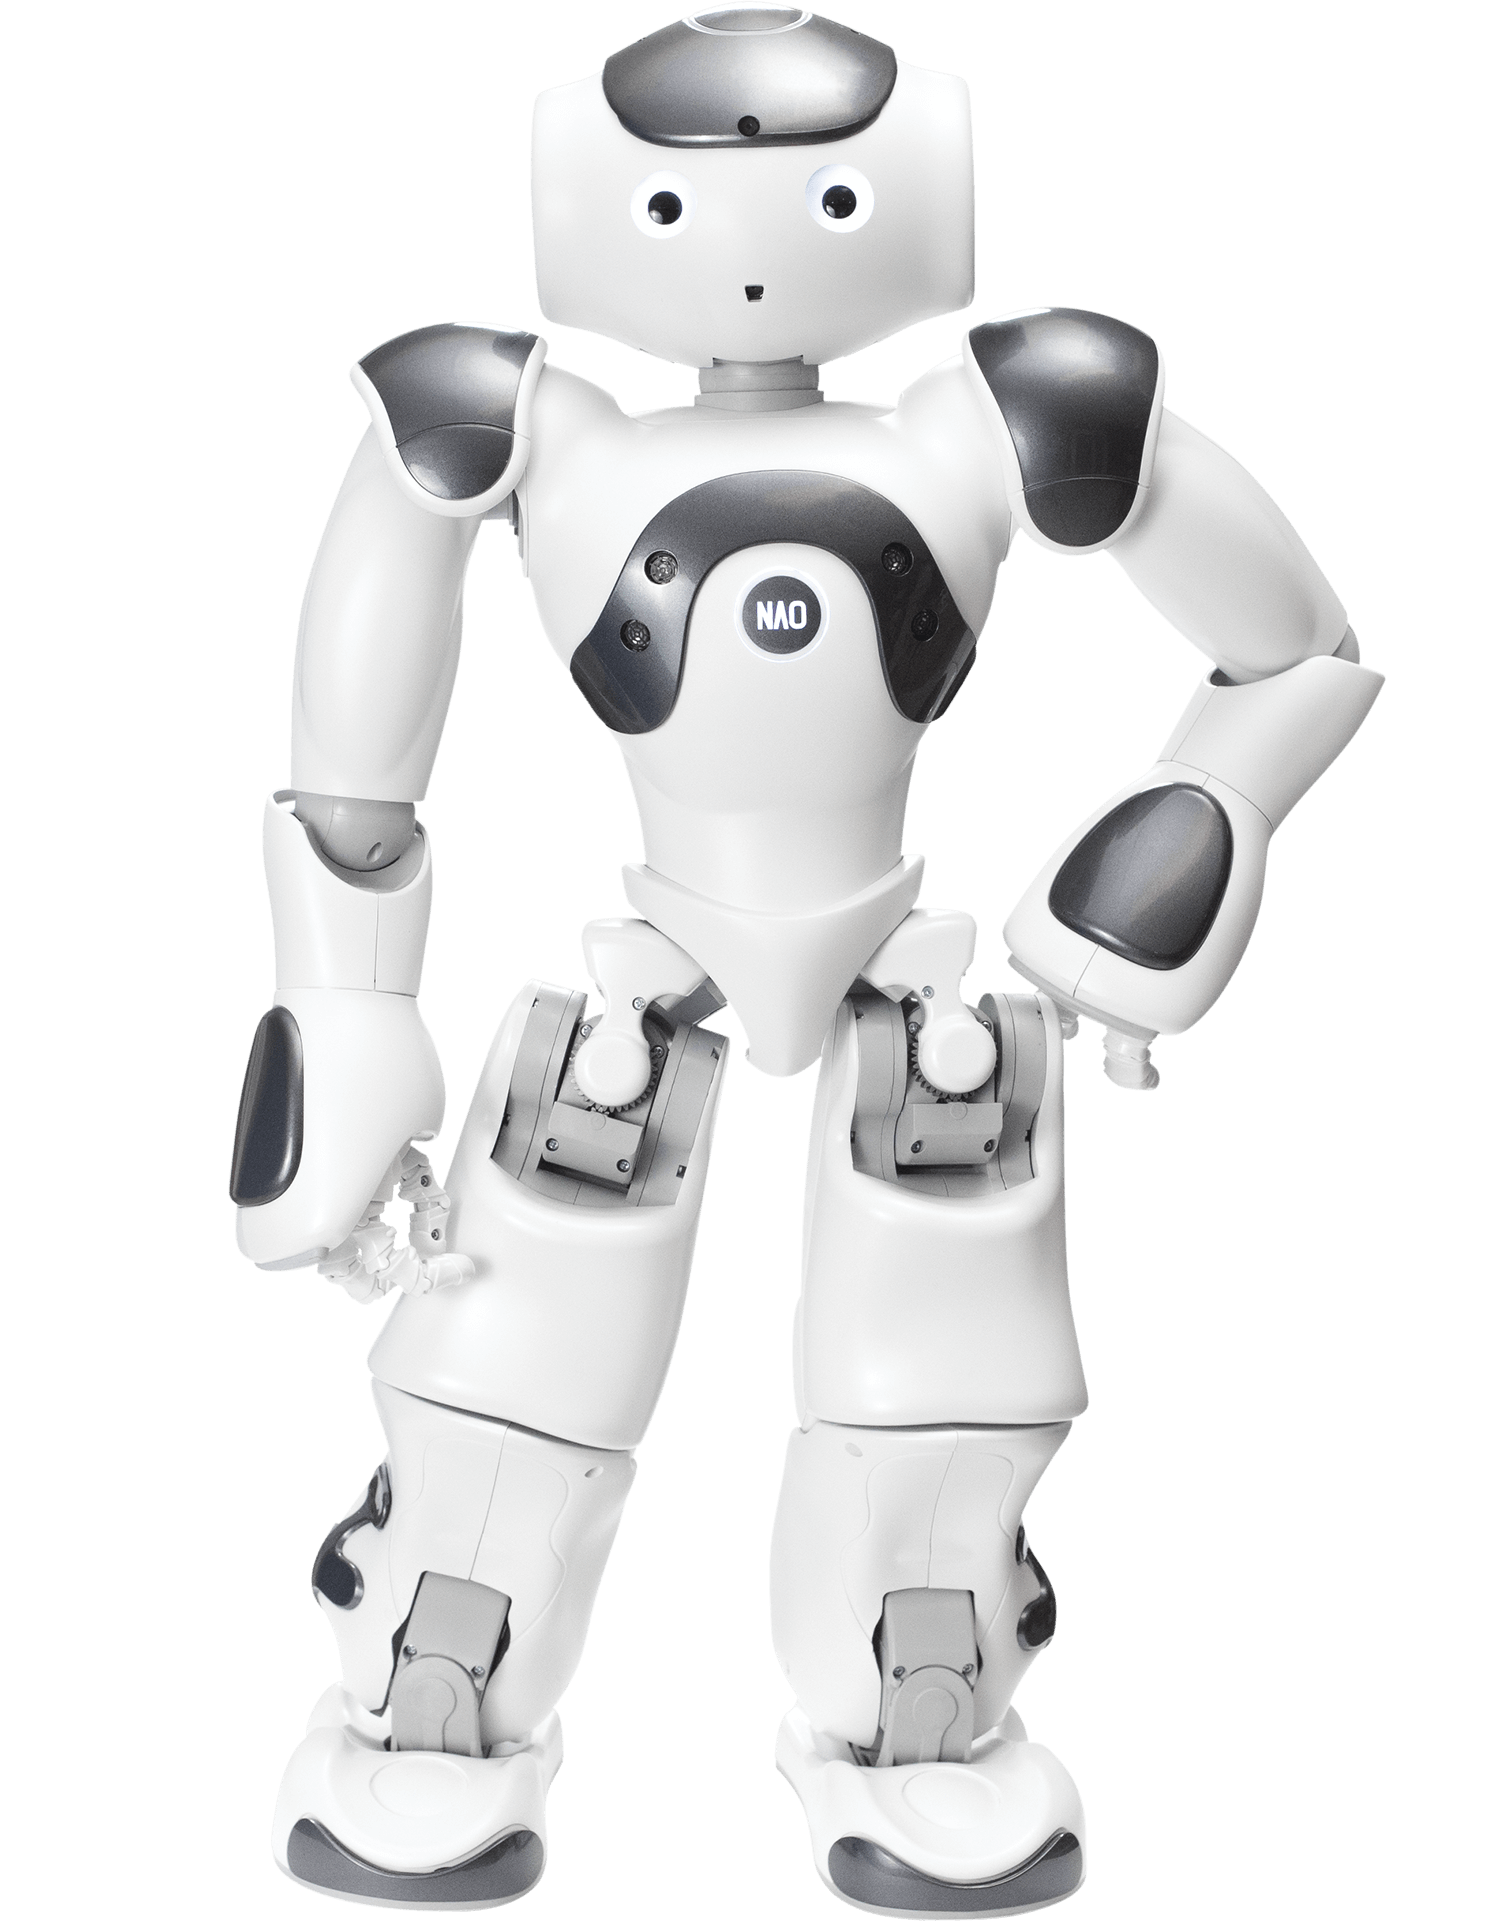
\includegraphics[width=0.8\textwidth]{img/robot.png}
    \caption{Imagen clásica de un robot} \label{fig:robot}
    \end{figure}

No hay un consenso sobre qué máquinas pueden ser consideradas robots,
dentro de este proyecto tomaremos como definición que un robot es un sistema autónomo programable capaz de realizar tareas complejas. Además, todos los robots se componen de tres partes esenciales  se componen de sensores, controladores y actuadores.
\begin{itemize}
    \item \textbf{Sensores}: Son los sentidos del robot, con ellos ve, escucha y sabe lo que hay en el entorno. Recogen la información necesaria para que el robot realice la tarea En este grupo se encuentran lásers, cámaras, ultrasonidos u odómetros..
    \item \textbf{Controladores}: El equivalente al cerebro humano, utiliza los datos recogidos por los sensores para elaborar una respuesta para que la lleve acabo los actuadores.
    \item \textbf{Actuadores}: Equivalen a los músculos humanos, son los que se encargan de interactuar con el entorno para llevar a cabo su tarea. Son brazos mecánicos, motores, etcétera...
\end{itemize}

\subsection{Aplicaciones robóticas}

Ahora que tenemos las bases de lo que es un robot asentadas podemos hablar de cuales son los principales propósitos de los robots hoy en día,aunque la mayor parte de ellos son utilizados por empresas en labores industriales. Aunque hay otros que podemos encontrar en nuestra vida cotidiana, en casas, hospitales, almacenes de tiendas... Esto es debido a la precision de algunos trabajos, la eficiencia en el trabajo, la reducción de costes que supone o que pueden realizar acciones de alto riesgo para las personas. Los ejemplos mas famosos en estos campos son los siguientes:
\begin{itemize}
    \item Robots Domésticos: Creados para realizar las tareas del hogar. Los mas famosos y destacados en el mercado son los Robots \textit{Roomba}, aspiradores autónomos, y también el primer robot que se ha comercializado para todos los públicos y de manera global. Un gran paso para la robótica

\begin{figure}[H]
    \centering
    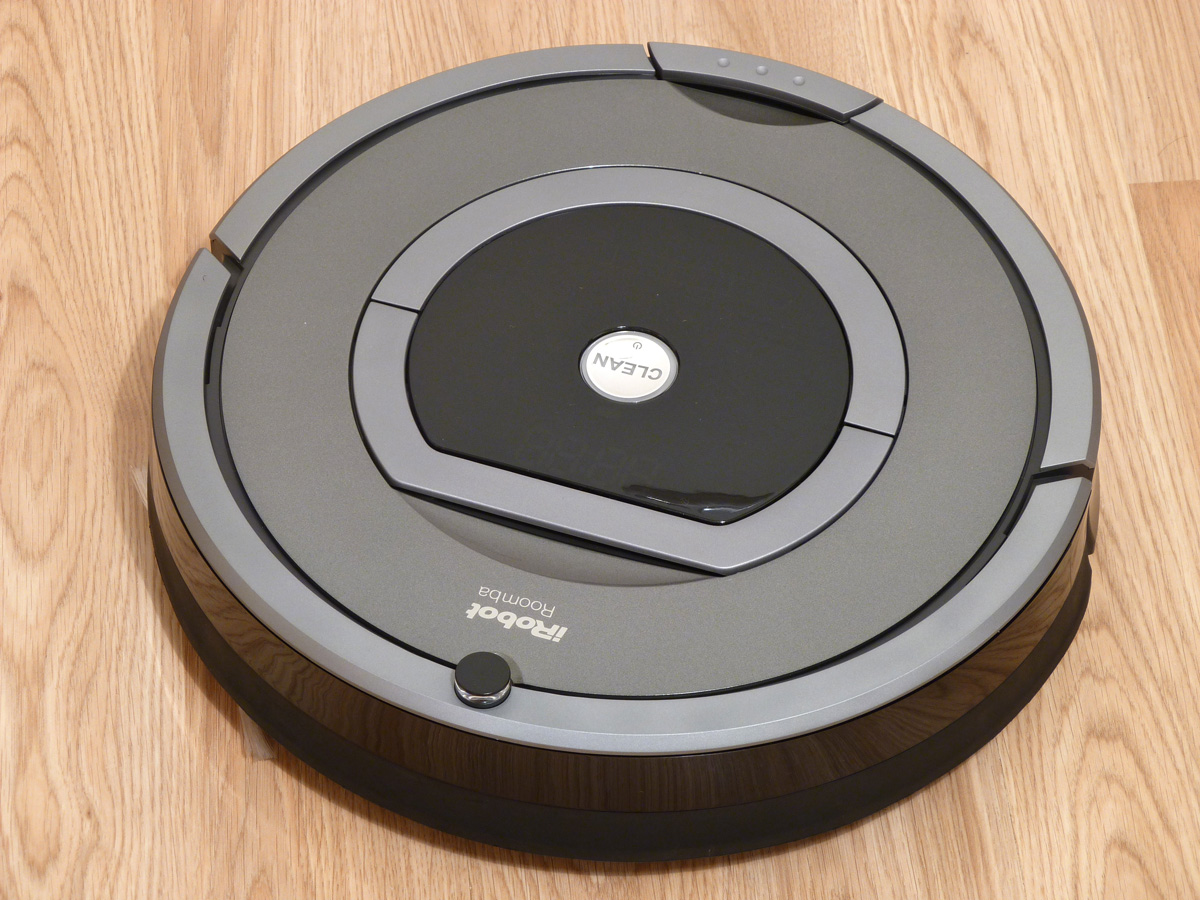
\includegraphics[width=0.6\textwidth]{img/roomba.jpg}
    \caption{Aspiradora robótica \textit{Roomba}} \label{fig:roomba}
    \end{figure}

    \item Robots médicos: Son robots diseñados para el uso en medicina para realizar tareas que requieren mucha precision como en el caso de una cirugía, con el robot \textit{Da Vinci} o robots diminutos que son capaces de navegar por las venas hasta llegar al corazón y allí realizar la cirugía necesaria.
      \begin{figure}[H]
    \centering
    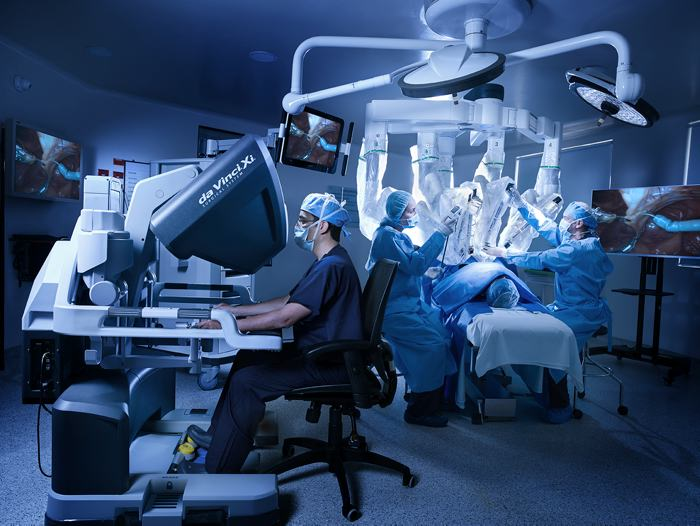
\includegraphics[width=0.6\textwidth]{img/davinci.jpg}
    \caption{Robot médico \textit{Da Vinci}} \label{fig:davinci}
    \end{figure}
    
    \item Robots militares: Son robots orientados a tareas militares, como reconocimientos de zonas conflictivas o rescate de personas, desactivación de bombas. En los últimos años también se han desarrollado mucho los drones en combate.
      \begin{figure}[H]
    \centering
    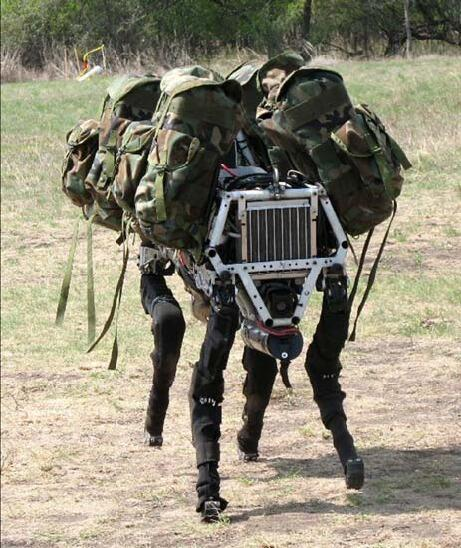
\includegraphics[width=0.6\textwidth]{img/bigdog.jpg}
    \caption{Robot militar \textit{Big Dog} creado por \textit{Boston Dynamics}} \label{fig:bigdog}
    \end{figure}
    
    \item Vehículos autónomos: Es el campo de la robótica que más en auge esta ahora mismo. El objetivo de estos robots es usar la información que proporcionan sus sensores internos, como cámaras, sensores infrarrojos \textit{Lidar}, y sensores externos como el GPS para llevar de un punto a otro un vehículo.

    \begin{figure}[H]
        \centering
        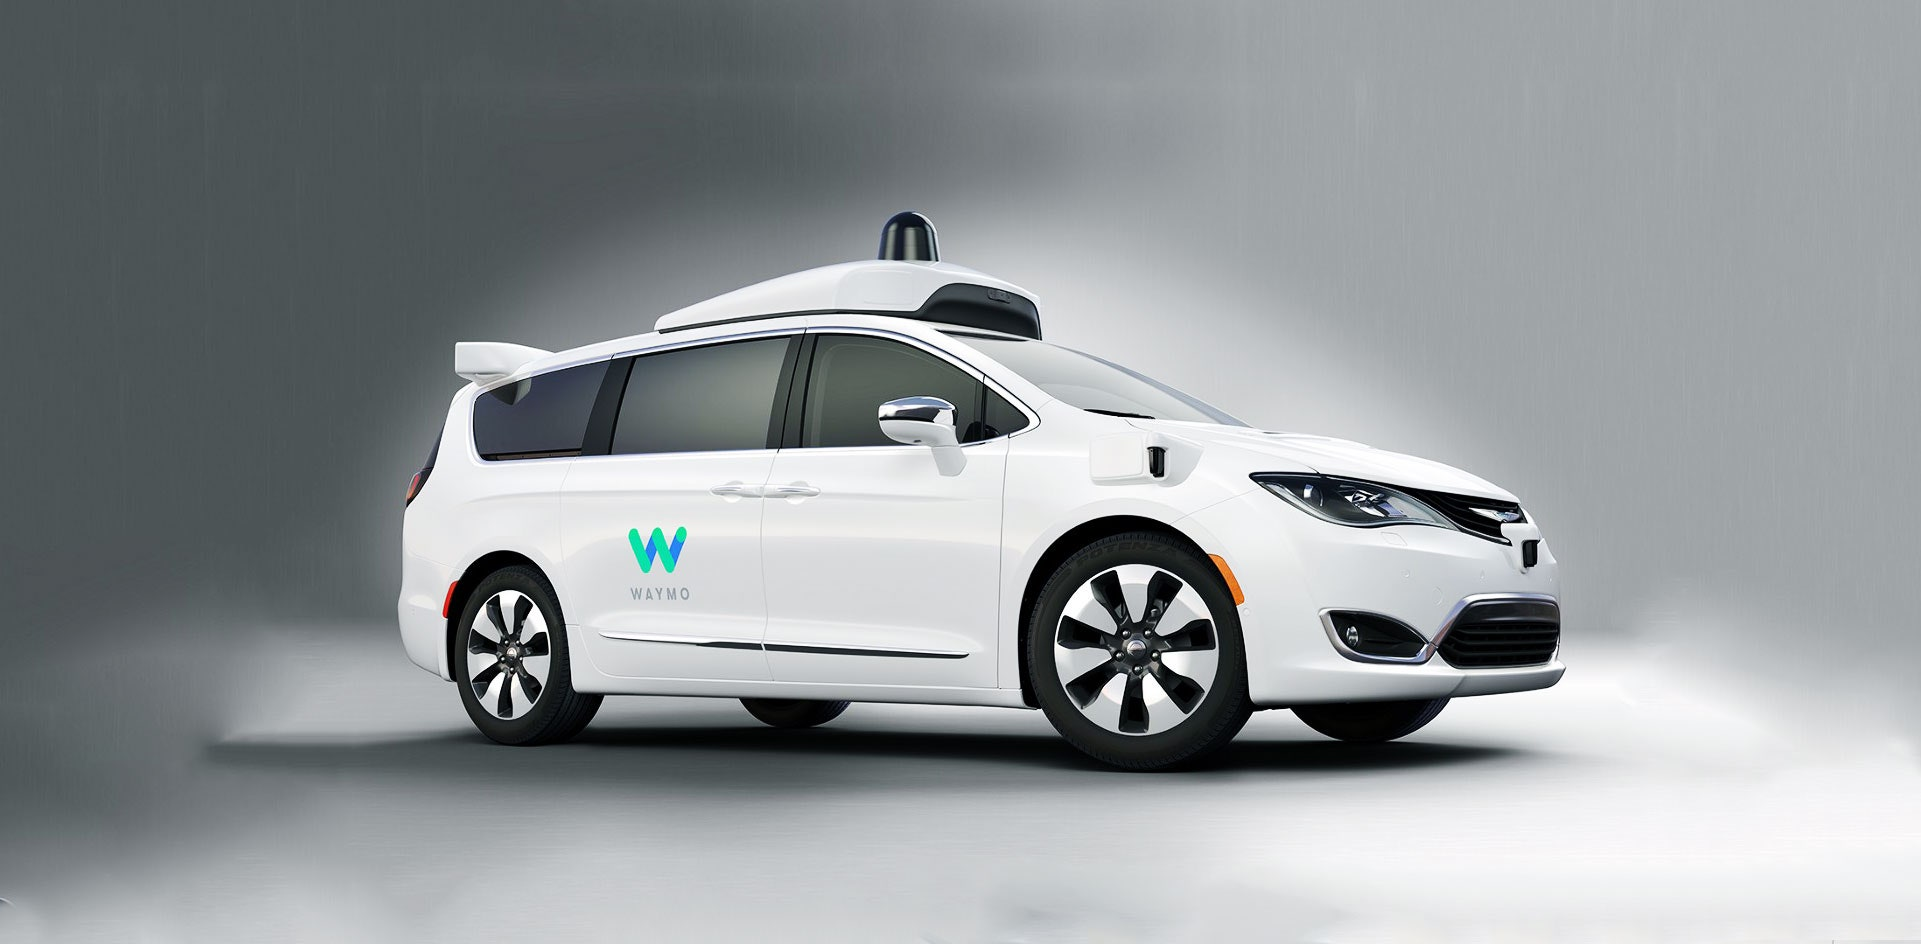
\includegraphics[width=0.7\textwidth]{img/waymo.jpg}
        \caption{Vehículo \textit{Waymo} de \textit{Google}} \label{fig:waymo}
    \end{figure}

    \item Robots Espaciales: Los famosos \textit{Rover} de la \textit{NASA} son robots diseñados para entornos donde el ser humano no puede llegar. Se centran en reconocimiento del terreno y análisis de las muestras que recogen.
        \begin{figure}[H]
    \centering
    \includegraphics[width=0.5\textwidth]{img/perseverance.jpg}
    \caption{Robot \textit{Perseverance} de la \textit{NASA}} \label{fig:Perseverance}
    \end{figure}
\end{itemize}

\subsection{Software en robótica}
\label{subsec:softwarerobot}
Para dotar de esta inteligencia a los robots se necesitan herramientas que transformen los datos recibidos de los sensores en algo que puedan aplicar en los actuadores. Hace años, cada maquina tenía un software especifico con sensores y actuadores únicos para ese robot y esa tarea a desarrollar. Esto hacia, que aunque hubieras implementado el software para otros robots anteriormente, tuvieras que repetir el proceso con cada nuevo robot. Con los años se desarrollaron plataformas de software que permiten desarrollar de manera genérica para todos los robots, y actuando de mediador entre el robot y el software del creador,estos son los llamados \textit{middleware} que hacen que te puedas abstraer de los \textit{drivers} característicos de cada robot. Los middleware mas importantes a día de hoy son:
\begin{itemize}
    \item \textit{\textbf{Robot Operating System (ROS)}}\cite{bib:ros}. Plataforma de \textit{software} libre para el desarrollo de \textit{software} de robots. Provee servicios estándar de un sistema operativo como la abstracción de \textit{hardware}, control de dispositivos de bajo nivel, mecanismos de intercambio de mensajes entre procesos y mas herramientas vitales para el desarrollo del robot. Es el mas utilizado a día de hoy porque fue especialmente desarrollado para \textit{UNIX} y luego se implemento para el resto de sistemas operativos
    \item \textit{\textbf{ORCA}}\cite{bib:orca}. Plataforma de \textit{software} libre diseñado para crear aplicaciones mas complejas, ya que esta orientado a las componentes por separado
     \item \textit{\textbf{OROCOS}}\cite{bib:orocos} Proyecto de \textit{software} libre también orientado a componentes y basado en C++

\end{itemize}{}

\subsection{Simuladores robóticos}
\label{sec:simuladores}
La simulación  es el proceso de diseñar un modelo de un sistema real y llevar a término experiencias con él, con la finalidad de comprender el comportamiento del sistema o evaluar nuevas estrategias. De esta forma los simuladores ahorran tiempo porque puedes detectar posibles errores en el código antes de lanzarlo en el \textit{Hardware} y que pueda llevar mayores problemas.\newline
Algunos de los simuladores que más se utilizan y más nos interesan en este proyecto:
\begin{itemize}
    \item \textbf{Gazebo}: Gazebo es un simulador de robótica 3D de código abierto. Gazebo fue un componente en el Proyecto Player desde 2004 hasta 2011. Gazebo integró el motor de física ODE, la representación de OpenGL y el código de soporte para la simulación de sensores y el control del actuador. También es importante destacar que tiene soporte para \texttt{ROS} lo que significa que puedes probar código real del robot en el simulador
    \begin{figure}[H]
    \centering
    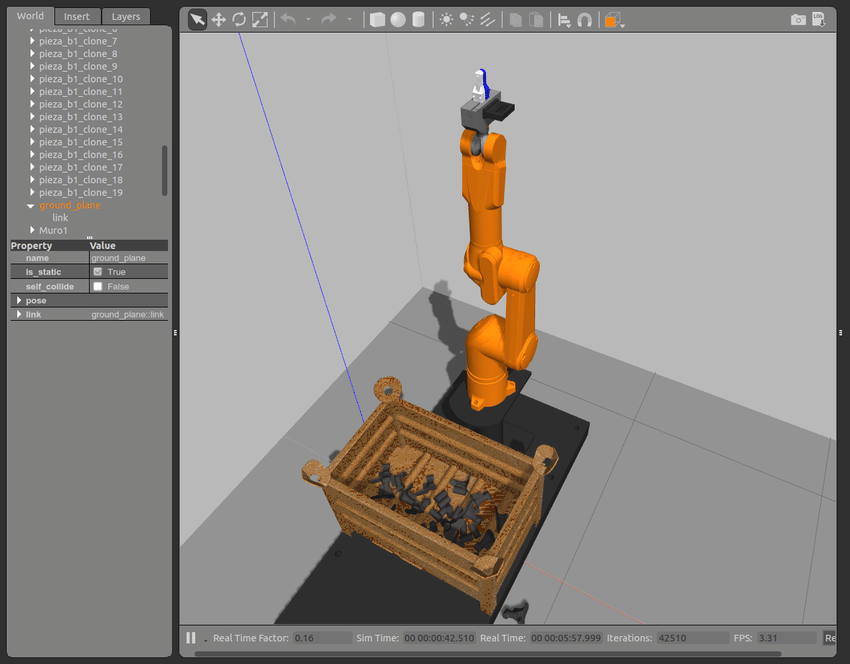
\includegraphics[width=0.7\textwidth]{img/gazebo.png}
    \caption{Interfaz de Gazebo} \label{fig:gazebo}
    \end{figure}
    
    \item \textbf{WebSim}: Es un simulador diseñado por alumnos de la universidad y que va escalando poco a poco. Hace uso de un entorno A-Frame y su diseño permite conectarlo con un editor que permite programar en diferentes lenguajes como \textit{JavaScript} y \textit{Python}, incluso un lenguaje de bloques llamado \textit{Blockly}(equivalente a Scratch pero diseñado por Google). Permite acoplar una aplicación externa a través de comunicaciones ICE. Es la base de la plataforma de \textit{Kibotics} y que vamos a utilizar en este proyecto.
\end{itemize}

\section{Tecnologías web}
\label{sec:web}
Las tecnologías web sirven para acceder a los recursos de conocimiento que hay disponibles en \textit{Internet} utilizando un \textit{navegador}. Son herramientas que procesan y lo muestran mediante una interfaz gráfica lo almacenado en un servidor. Además gracias a la forma que esta estructurada la \textit{World Wide Web} (WWW) hace sencillo saltar de un recurso a otro. 
WWW es una combinación de 4 ideas: Hipertexto, identificadores de recursos(URL y URI), el lenguaje de marcado y el modelo cliente servidor.

\begin{figure}[h]
\centering
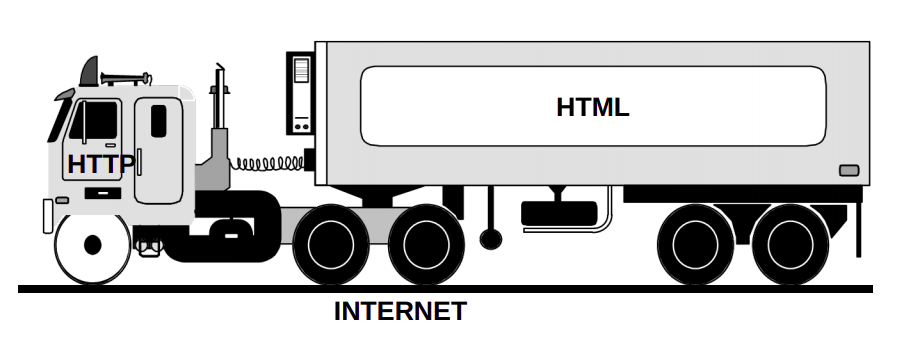
\includegraphics[scale=0.4]{img/tecnologiasweb.png}
\caption{Concepto de Tecnologias Web} \label{fig:tecnologiasweb}
\end{figure}

Lo que nos interesa de las \textit{Tecnologías Web} es el modelo de cliente-servidor, también llamados, \textit{FrontEnd} a todo lo que el usuario se encuentra directamente en la web, lo que es la parte del cliente. Y \textit{BackEnd} a la parte del interior de las aplicaciones que viven en el servidor, que es lo denominado "el lado del servidor". Modelo que utilizare para abastecer a mi robot de los programas que se desarrollan en \textit{Kibotics}.
\subsection{FrontEnd}
\label{subsec:frontend} 
Es la parte encargada de dar forma a la interfaz de usuario y de establecer la comunicación con el servidor. Una pieza importante del cliente es el navegador, ya que es el encargado de leer e interpretar la información recibida. Entre los navegadores \textit{web} más empleados se encuentran \textit{Firefox}, \textit{Google Chrome} u \textit{Opera}\cite{bib:navegadores}. Las tecnologías que hacen posible esa comunicación son: 

\begin{itemize} 
    \item \textit{\textbf{JavaScript}}. Es un lenguaje de programación interpretado, dialecto del estándar ECMAScript. Se define como orientado a objetos. Es el lenguaje más utilizado para el desarrollo de aplicaciones Web y de paginas Web. La mayor parte de \textit{Kibotics} esta desarrollado en \textit{Javascript}. Por lo que en el siguiente capítulo desarrollaremos en más profundidad.
    \item \textit{\textbf{HTML}}. siglas en inglés de HyperText Markup Language, hace referencia al lenguaje de marcado para la elaboración de páginas web. Es el estándar más utilizado a dia de hoy.\newline
HTML sólo sirve para indicar como va ordenado el contenido de una página web. Esto lo hace por medio de las marcas de hipertexto las cuales son etiquetas conocidas en inglés como tags. Las mejoras del diseño gráfico ya vienen dada de la versión actual, \textit{HTML5}, que incluye muchas mejoras respecto a su predecesor: \textit{canvas}, \textit{websockets}, \textit{WebRTC}, vídeo, audio, etc. Este lenguaje indica la estructura de una página web, para editar el estilo y presentación visual hay que hacer uso de otros elementos como \textit{CSS}.
    \item \textit{\textbf{Cascading Style Sheets (CSS)}}. Lenguaje de diseño gráfico para definir y crear la presentación de un documento escrito en un lenguaje de marcado. De esta forma, se puede separar información y datos (en los documentos \textit{HTML}) y todo lo relativo al diseño y presentación (en documentos \textit{CSS}). Actualmente los navegadores usan la versión \textit{CSS3}.

\end{itemize}

\begin{figure}[h]
\centering
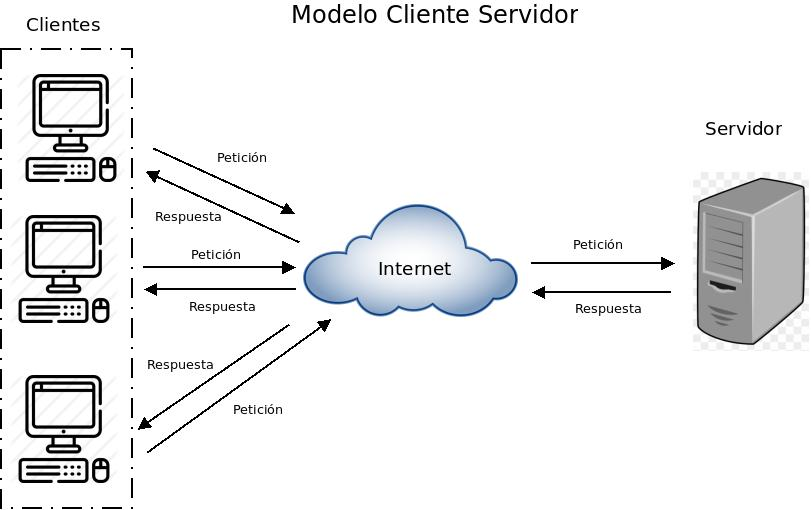
\includegraphics[scale=0.4]{img/http.jpeg}
\caption{Comunicación cliente-servidor en HTTP} \label{fig:http}
\end{figure}
\subsection{BackEnd}
\label{subsec:backend}
En la parte del servidor web se encarga de proveer los datos, hacer posible crear una aplicación que se le mostrará al cliente y facilitar herramientas como bases de datos y recursos compartidos. 
\begin{itemize}
    \item \textbf{Node.js}: Node. js es un entorno JavaScript que nos permite ejecutar en el servidor, de manera asíncrona, con una arquitectura orientada a eventos   
    \item \textbf{Django}: Django es un framework web extremadamente popular y completamente funcional, escrito en  \textit{Python}. El módulo muestra por qué Django es uno de los frameworks de servidores web más populares.
\end{itemize}

\subsection{HTTP}
\label{subsec:http}

\textit{HiperText Transfer Protocol} (\textit{HTTP}) es el protocolo de nivel de aplicación utilizado para transferir recursos hipermedia entre ordenadores y sigue el esquema petición-respuesta entre cliente y servidor (Figura \ref{fig:http}). 
Las peticiones están definidas por el protocolo y tienen métodos concretos: 
\begin{itemize}
    \item GET: Solicita un recurso al servidor especificando su \textit{URL}.
    \item HEAD: Método similar a GET con la diferencia de que únicamente solicita las cabeceras y no descarga el recurso completo.
    \item POST: Envía datos al servidor, normalmente un recurso específico que provoca un cambio de estado. Es también bastante similar GET pero la cabecera va en claro. 
    \item PUT: Actualiza información sobre un recurso del servidor. 
    \item DELETE: Elimina en el servidor un recurso.
\end{itemize}

Aunque estos son los principales métodos, el protocolo tiene flexibilidad para ir añadiendo nuevos e incorporar funcionalidad. El número de métodos ha ido aumentando con las nuevas versiones.\newline




\section{Robótica educativa}
\label{sec:educativa}
La robotica educativa ha ido tomando mas importancia con los años, ya que cada vez es mas importante que estudiantes de cualquier nivel estén familiarizados con la tecnología, tiene valores positivos como la implementación de pensamiento lógico, resolución de problemas y trabajo en equipo en las actividades académicas, que son ramas del conocimiento que se desarrollan poco en edades tempranas , con una componente en conocimiento matemático y físicos y ademas añade un atractivo que no tienen las asignaturas convencionales.
Muchos estudios han demostrado que el uso de kits de robótica en la educación favorece a la capacidad de reflexión de los estudiantes.
Cada año se crean mas cursos de robótica, y en 2015 la comunidad de Madrid introdujo la asignatura de robótica en los planes docentes de Enseñanza Secundaria con la asignatura ``Tecnología, Programación y Robótica''\cite{bib:secundaria} y en el curso 2020-2021 se empezará a implantar en Educación Primaria la asignatura ``Programación y Robótica''\cite{bib:primaria}.\newline
Este tipo de educación es el llamado modelo \textbf{STEM}(siglas de \textit{Science, Technology, Engineering y Mathematics}), término creado por Seymound Papert en la década de los 80 cuando creo uno de los primeros juguetes con programación incorporada, creada para niños, el llamado \textit{"Lego-Logo"}, dando mucha importancia a juegos con engranajes, que consideraba que enriquecía el pensamiento. Justamente, el referente del protagonista de este proyecto.\newline
Pero no fue hasta 2010, cuando este modelo de educación empezó a tomar relevancia, y se inicio la inclusión en la agenda escolar.
        \begin{figure}[H]
    \centering
    
\includegraphics[width=0.7\textwidth]{img/stem.jpg}
    \caption{Modelo de Educación \textit{STEM}} \label{fig:stem}
    \end{figure}
Una de las mayores partes de la robótica tiene que ver con la programación, que ademas de ser una habilidad muy importante para la sociedad actual, es algo complejo. Por lo que se utilizan lenguajes de programación visual, estos se tratan de lenguajes que abstraen en bloques las funciones o métodos de cualquier lenguaje de programación. Dentro de este tipo de lenguajes, los mas destacables son :

\begin{itemize}
    \item \textit{\textbf{Scratch}}\cite{bib:scratch}: proyecto liderado por el Grupo \textit{Lifelong Kindergarten} del \textit{MIT}, es utilizado por estudiantes para programar animaciones, juegos e interacciones. Su atractivo reside en lo facil que es de entender el pensamiento computacional debido a su sencilla interfaz gráfica y la implementación de sus bloques.
    \begin{figure}[H]
    \centering
    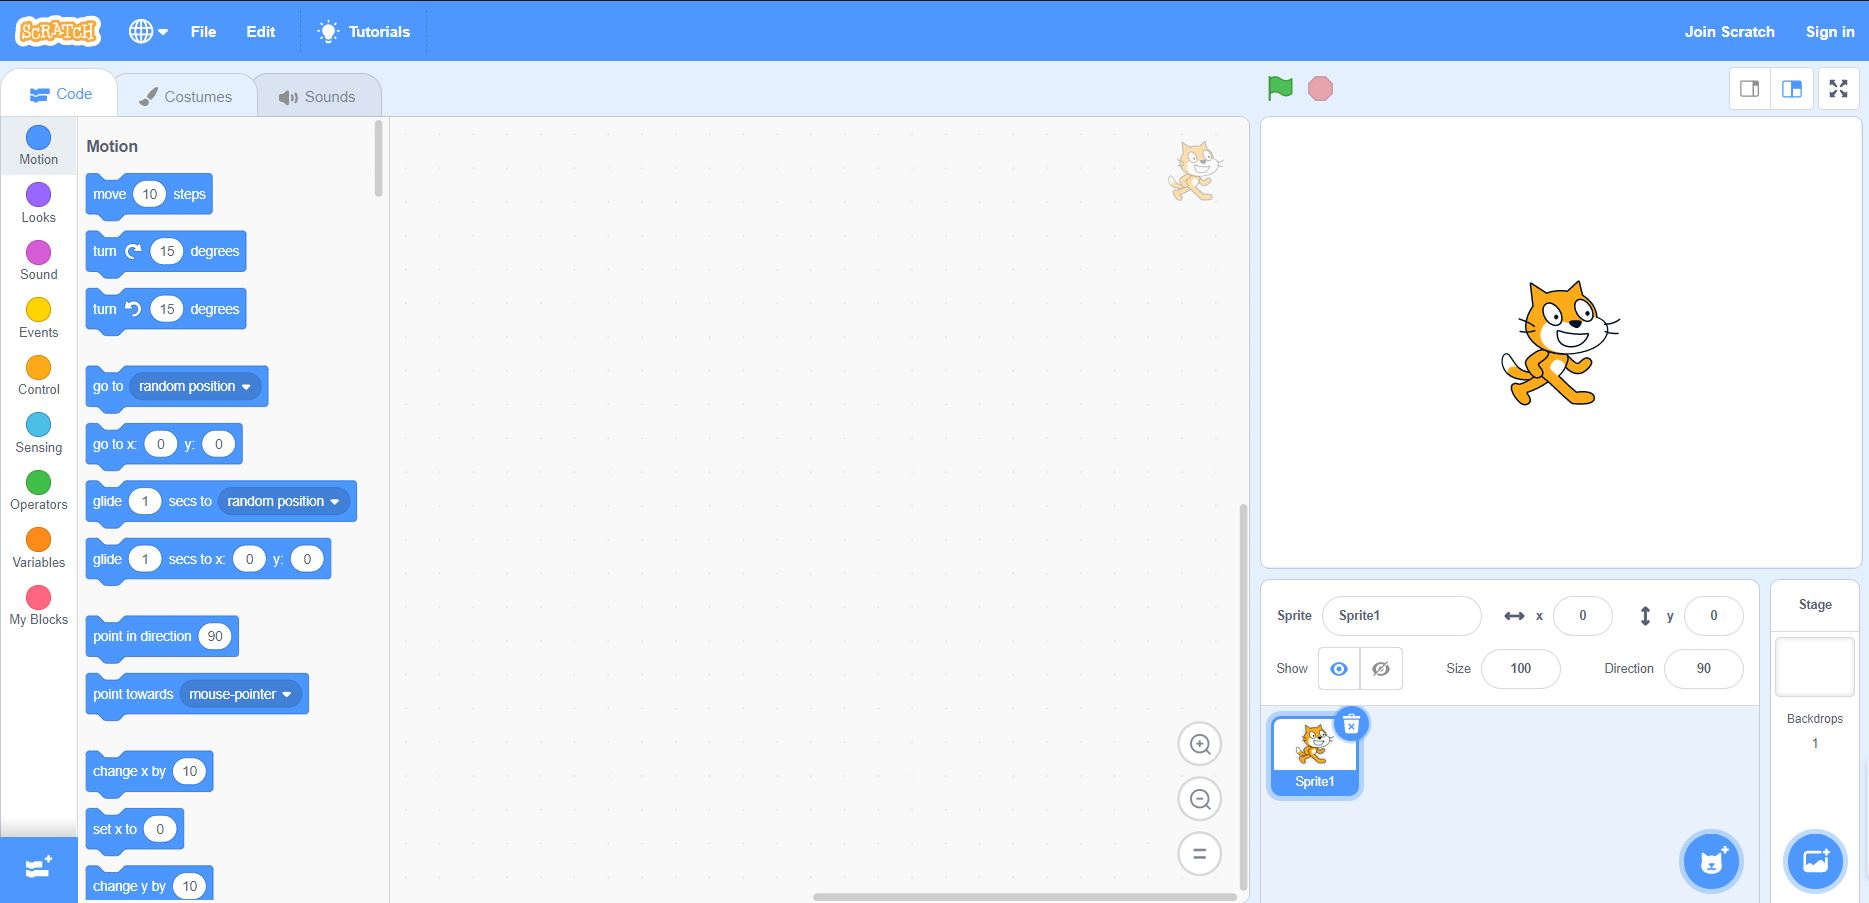
\includegraphics[width=0.7\textwidth]{img/scratch.jpg}
    \caption{Interfaz gráfica de Scratch} \label{fig:scratch}
    \end{figure}

    \item \textit{\textbf{LEGO}}\cite{bib:lego}: Es el robot base de este proyecto,dispone de una amplia gama de robots programables y cada uno de ellos tiene un sistema gráfico, que es similar entre ellos pero también ligado a la edad el estudiante para el que esta diseñado el software. 

    \begin{figure}[H]
    \centering
    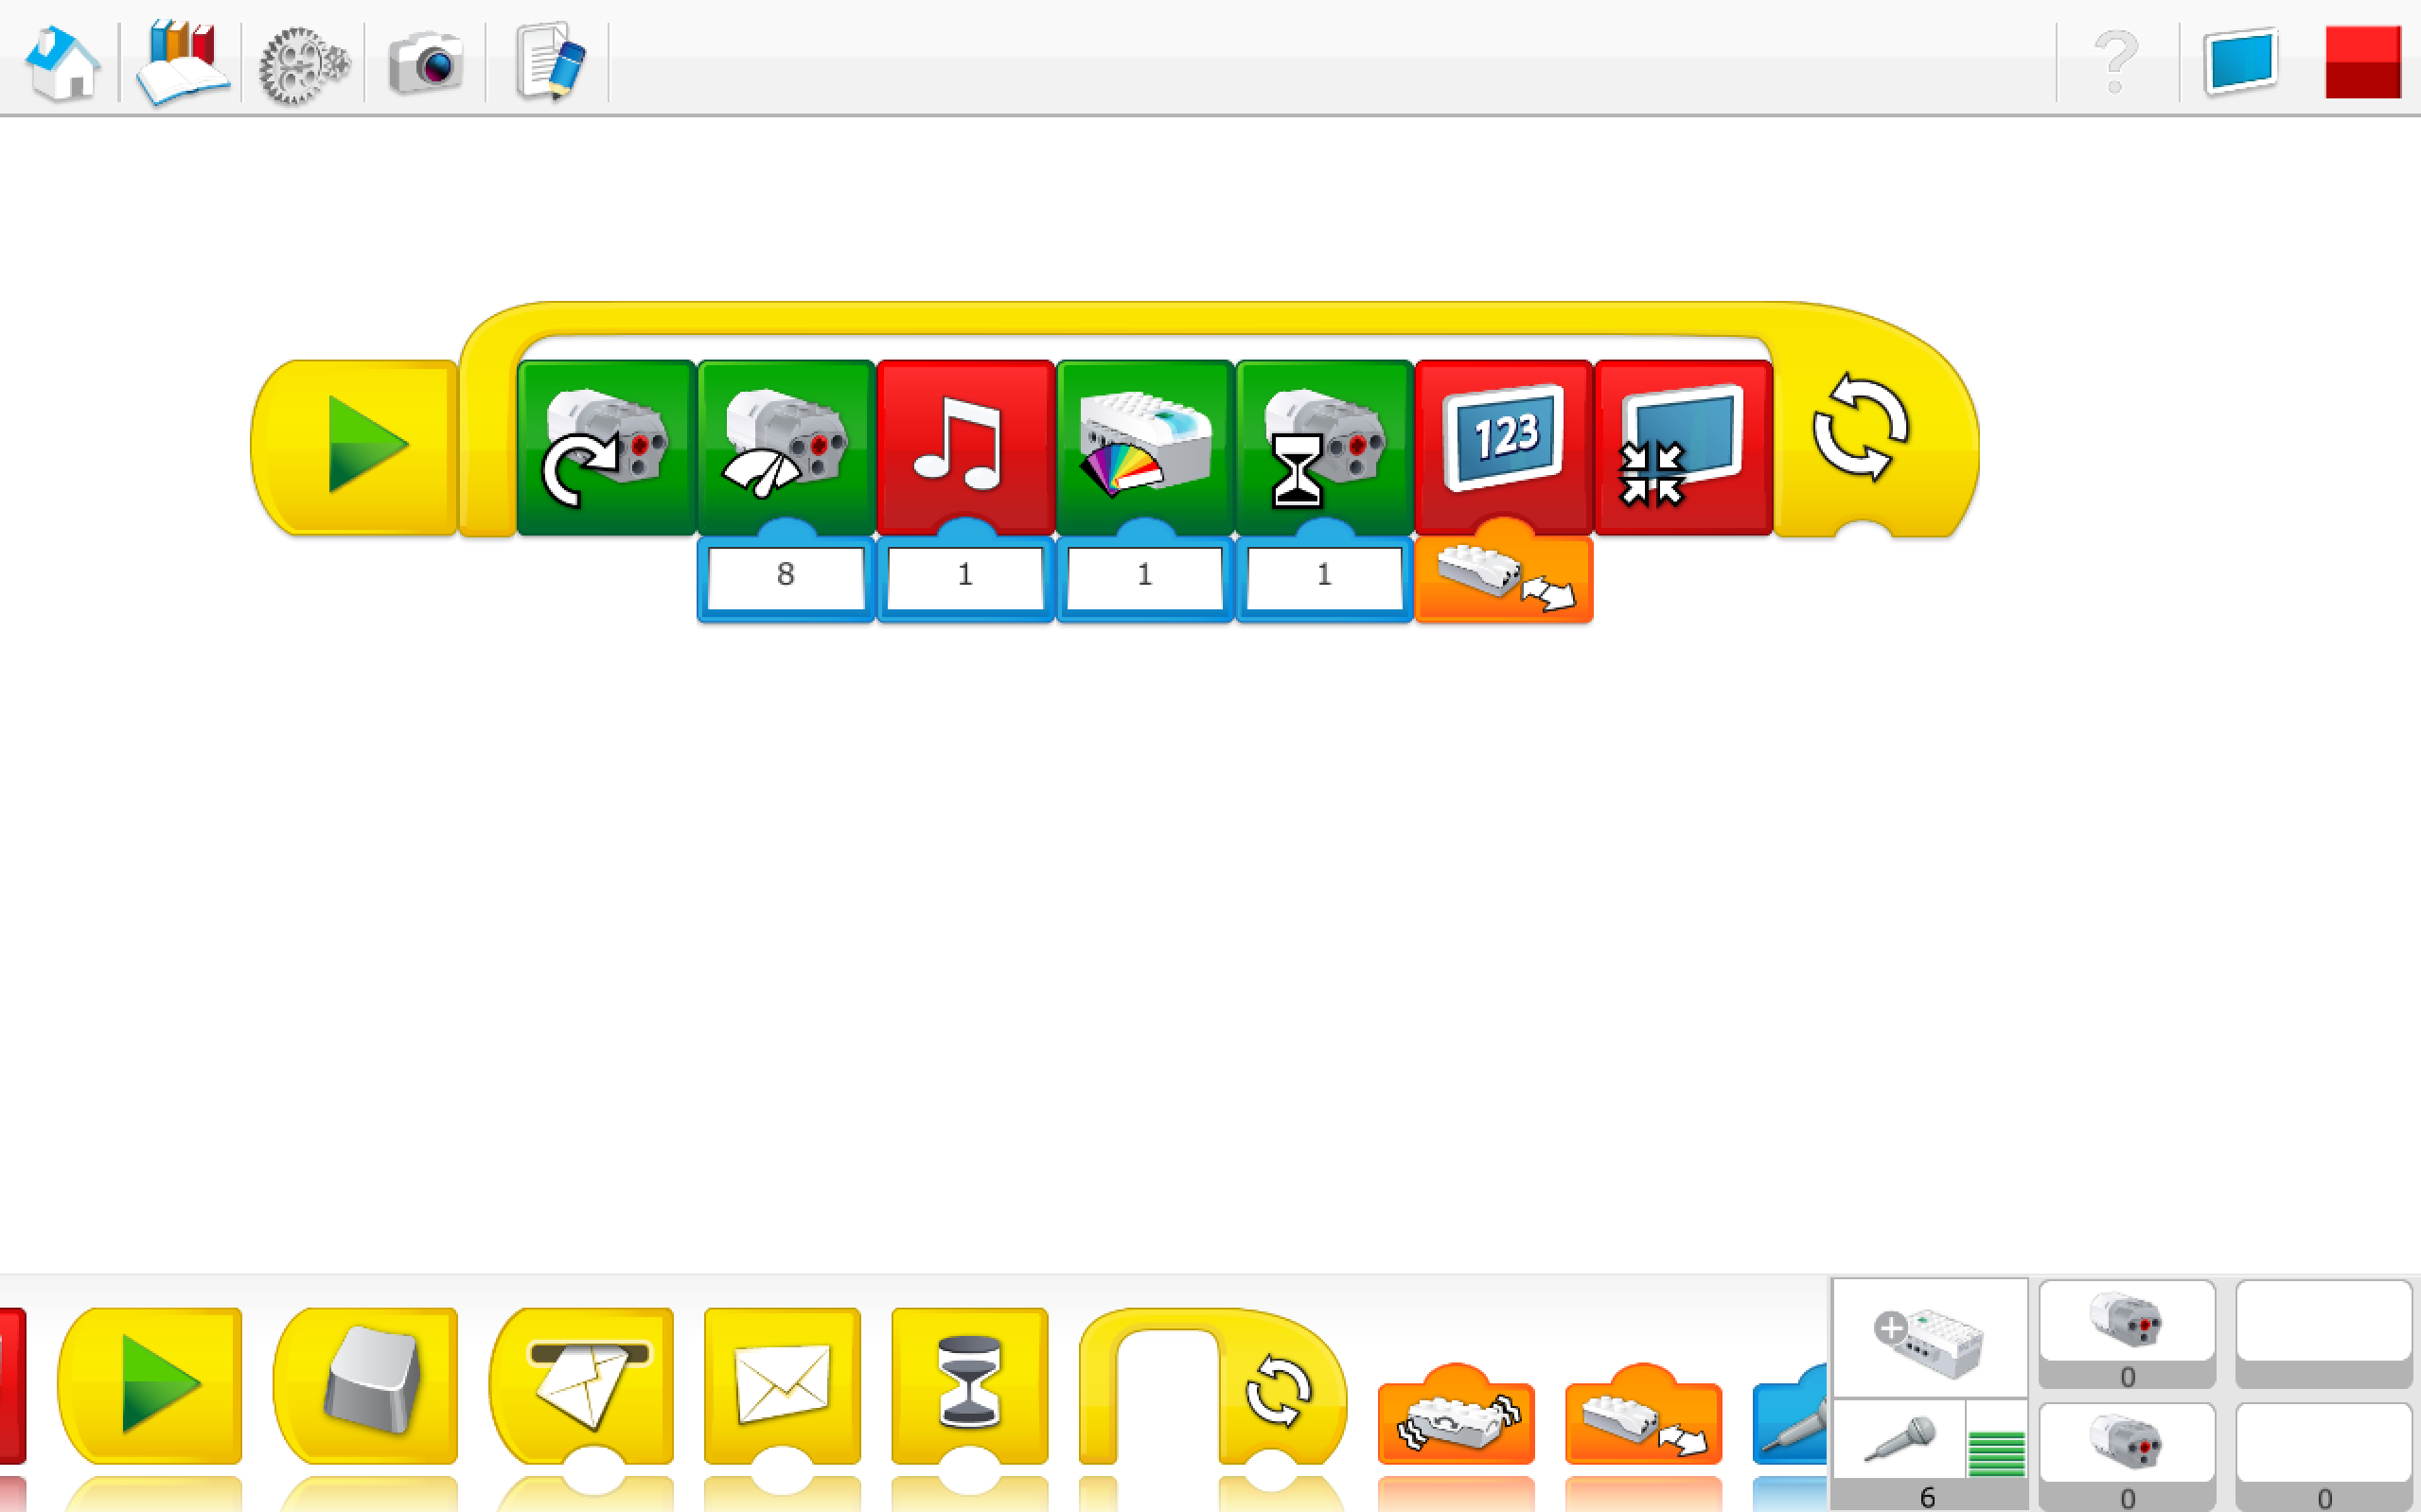
\includegraphics[width=0.7\textwidth]{img/lego1.png}
    \caption{Interfaz de LEGO WeDo} \label{fig:lego1}
    \end{figure}
    
Por ejemplo en la figura \ref{fig:lego1} se puede ver que la interfaz en este caso, es con colores vivos, los cuales representan distintas funcionalidades dentro del robot, es decir, el amarillo representa las acciones propias de programación, como: inicio de programa, fin de programa, bucles, esperar, etcétera. El color rojo representa los sensores del robot, todo lo que recoja datos. Y el color verde representa los motores que equivalen a los actuadores en este robot.
Como se puede observar es una abstracción muy simple para estudiantes de mas corta edad.
	 \begin{figure}[H]
    \centering
    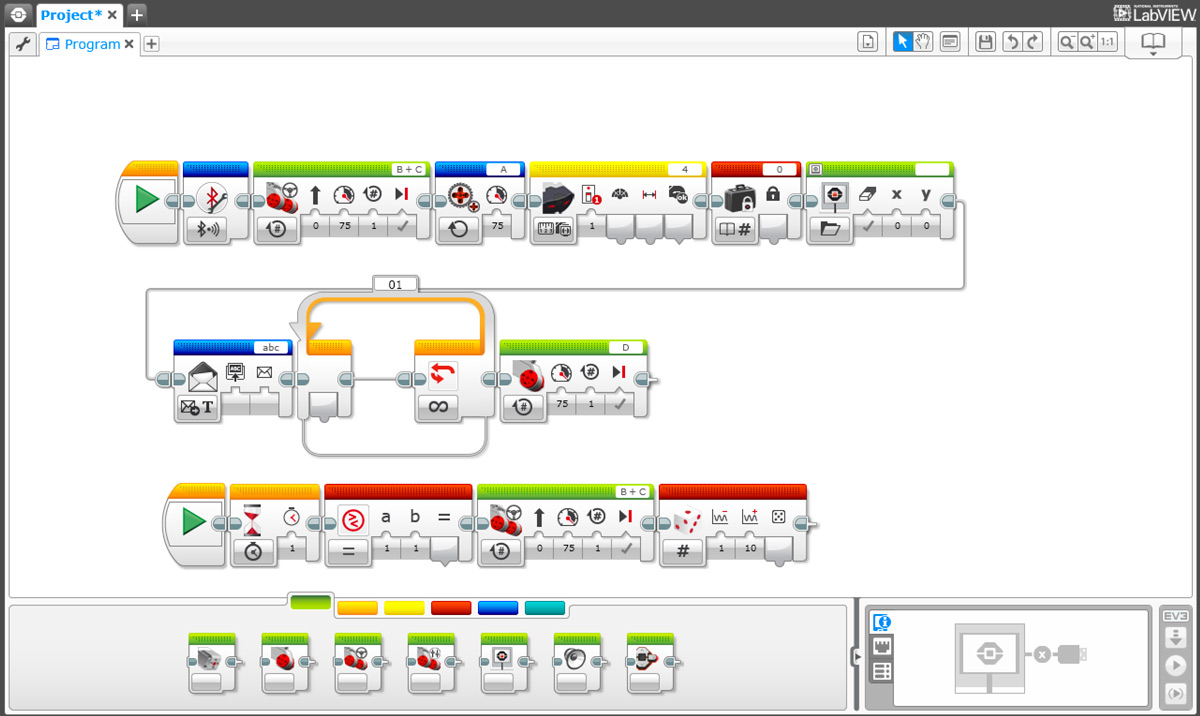
\includegraphics[width=0.7\textwidth]{img/lego2.jpg}
    \caption{Interfaz gráfica de LEGO Ev3} \label{fig:lego2}
    \end{figure}

En el caso del software para el \textbf{LEGO Ev3}, añade un grado de complejidad, incluyendo apartados para realizar operaciones matemáticas, envio de archivos entre robots, y añade mas actuadores, como la pantalla que integra el robot, o los altavoces.

En el caso de LEGO y en otros kits incorporan los elementos básicos para la construcción de un robot. En este en particular viene con lo indispensable para construir con piezas de LEGO. También incluye un microprocesador para ser programado, con Linux instalado, sensores (infrarrojos, táctiles y de color) y motores.
  \begin{figure}[H]
    \centering
    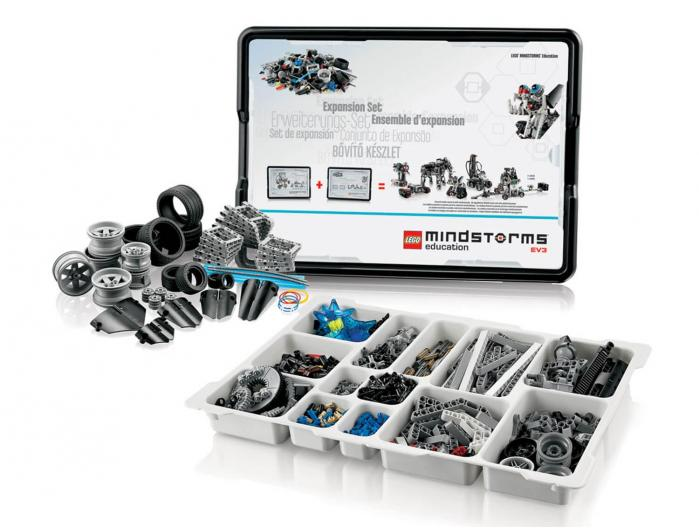
\includegraphics[width=0.7\textwidth]{img/kitev3.jpg}
    \caption{Kit de piezas y sensores de LEGO Ev3} \label{fig:lego3}
    \end{figure}
\end{itemize}{}


En el siguiente capitulo, profundizare mas en lo que se puede hacer con el robot \textbf{LEGO Ev3} y explicare cuales van a ser los objetivos y porque elegir este robot.



\subsection{Kibotics}
\label{sec:kibotics}
Kibotics\footnote{\url{https://kibotics.org/}}, es un entorno web desarrollado por la Asociación JdeRobot\footnote{\url{https://jderobot.github.io/}} para la docencia de robótica. Fue creada para impartir cursos de robótica, en los que destacan una iniciación muy sencilla, y una gran variedad de recursos a disposición del alumno.
Es una plataforma en la que podemos encontrar distintos ejercicios de robots simulados que no son reales (como el Formula 1). Tiene los ejercicios divididos , en los robots con ruedas sobre una superficie, con cámaras, sensores de todo tipo, y los drones, con funcionalidad adicional, y otro tipo de ejercicios, y dentro de estos dos grupos, se dividen entre los dos lenguajes de programación. \newline
 
\begin{figure}[h]
  \centering
    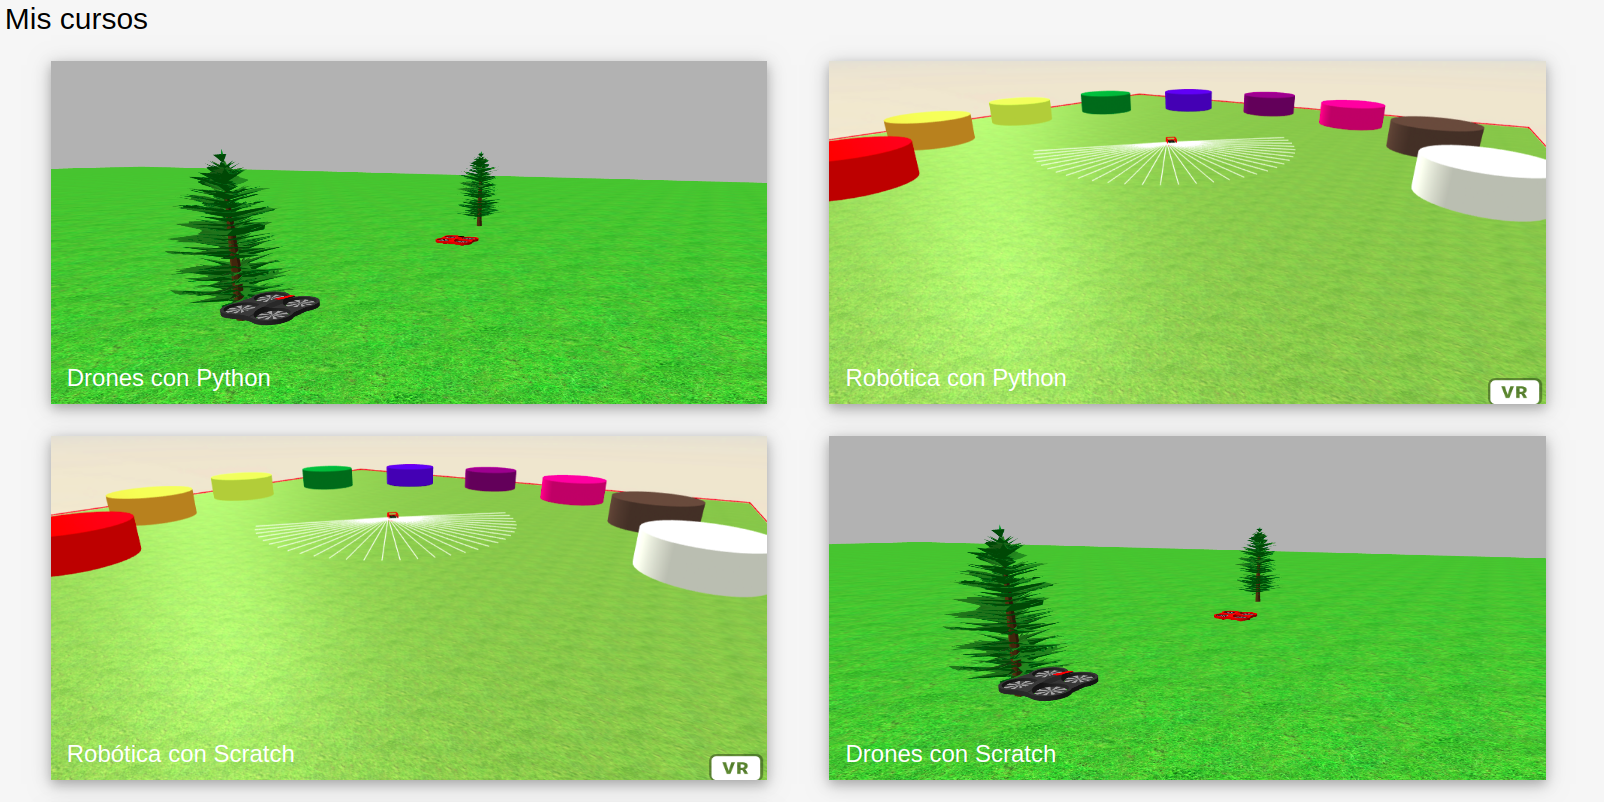
\includegraphics[width=1\textwidth]{img/kibotics2.png}
  \caption{Menu principal de \textit{Kibotics}}
  \label{Robot PiBot}
\end{figure}
En cuanto a los lenguajes reconocidos por esta plataforma, encontramos \textit{Blockly},el equivalente de \textit{Scratch} pero creada por \textit{Google}, un lenguaje de bloques. Su uso en colegios, para estudiantes de corta edad es cada vez más frecuente. También encontramos \textit{Python} un lenguaje de alto nivel, de los más populares actualmente. Es el que emplean los estudiantes más mayores. 
\begin{figure}[h]
  \centering
    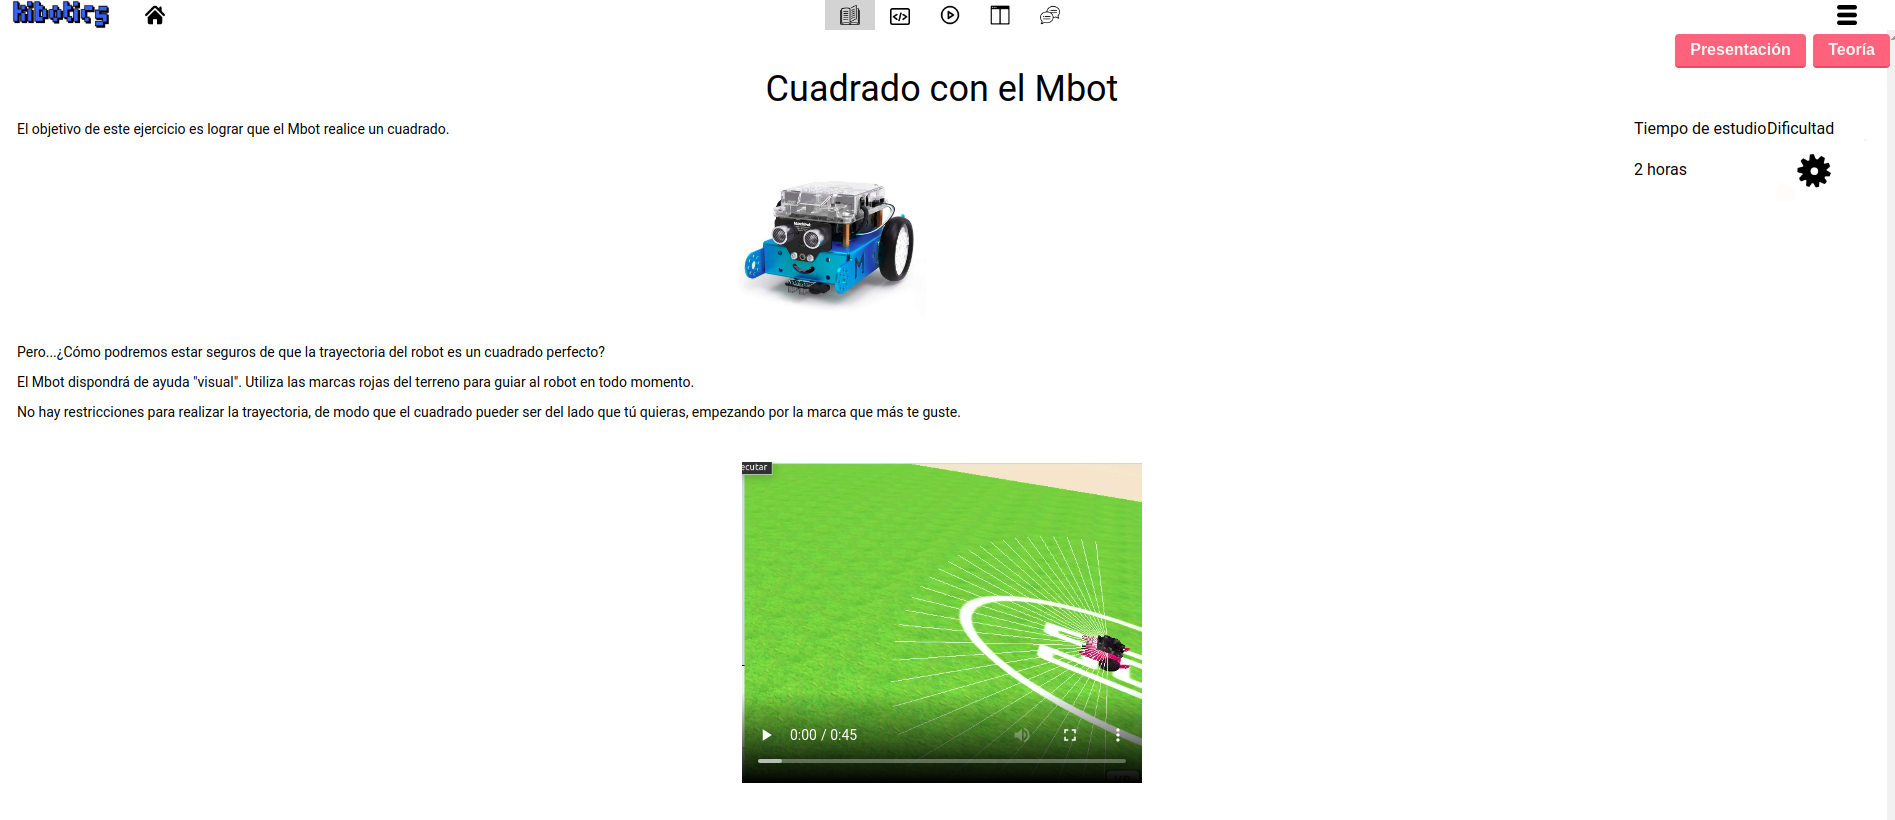
\includegraphics[width=1\textwidth]{img/kibotics1.png}
  \caption{Ejercicio en Kibotics}
  \label{Ejercicio con Blockly en Kibotics}
\end{figure}

Cada ejercicio viene con una parte teórica, donde se explica la lección que se va a aprender y los pasos para seguir para poder completar el ejercicio, la siguiente pestaña, es donde se programa el ejercicio, y la última, es donde se encuentra el simulador que ejecuta el código que acabas de programar.






% OBJETIVOS %
%%%%%%%%%%%%%%%%%%%%%%%%%%%%%%%%%%%%%%%%%%%%%%%%%%%%%%%%%%%%%%%%%%%%%%%%%%%%%%%%
\chapter{Objetivos}\label{chap:objetivos}
Una vez explicado en el ámbito en el que se realiza este proyecto, en este capitulo explicaremos los objetivos que se han tratado de alcanzar y el método de trabajo que se ha seguido para lograrlo

\section{Objetivos del TFG}
El objetivo de este trabajo es dar soporte en la plataforma de \textit{Kibotics} \footnote{\url{https://kibotics.org/}} a un robot bastante popular para la robótica educativa como es el \textit{LEGO Ev3}, esto significa integrarlo de forma que se pueda programar dentro de la plataforma, y que también funcione para el robot real.\newline 
\textbf{Soporte Simulado}
\begin{itemize}
    \item Añadir una simulación 3D realista sabiendo que hay modelos de robots prediseñados por \textit{LEGO} de varios modelos de robots, al menos uno por cada tipo de sensor que pueda llevar. Y que tenga sentido físico dentro de la simulación.
        
    \item Añadir la infraestructura necesaria como \textit{drivers}, y funciones al \textit{Robot API} para que el robot se programable en cualquier lenguaje soportado por la plataforma, y funcione en el robot real
    
    \item Crear un conjunto de ejercicios para que haya una comprobacion de que lo implementado funciona, y asi tener un temario fácil de seguir por el estudiante, y con una curva de dificultad moderada
    
\end{itemize}
\textbf{Soporte Real}
\begin{itemize}
    \item Instalar una imagen de un sistema operativo en el \textit{Lego ev3} en este caso, una distribución basada en \textit{Debian Linux}, e instalar lo necesario para que se ejecuten programas en \textit{Python}.
    \item Instalar un servidor en el robot capaz de recibir mensajes con el código, y lo transforme en un archivo y lo ejecute dentro de la máquina. Posteriormente, probar la ejecución enviando ejercicios desde el navegador.
    
\end{itemize}

\section{Requisitos}
\label{sec:requisitos}
Para completar la integración del robot \textbf{LEGO Ev3} se necesitan ciertos requisitos que cumplir:
\begin{itemize}
    \item Dentro del \textbf{LEGO Ev3} debe correr una distribución de \textit{Linux} , en este caso he optado por la imagen creada por \textit{ev3dev}, que es una distribución basada en el sistema operativo \textit{Debian Linux}, de la cual entrare en mas detalle en el Capitulo 5: \textit{Soporte Lego ev3 físico}.
\item Se deben crear todas las funciones necesarias para que todos los sensores incluidos en \textit{LEGO Ev3}, tengan equivalencia en la plataforma de \textit{Kibotics}.
\item Toda la funcionalidad que implemente en la plataforma debe ser comprobada mediante ejercicios que se realicen tanto en la plataforma, como en el robot real.
    \item El resultado final debe ser lo más sencillo posible, no debe requerir configuraciones adicionales. Este software tiene que estar diseñado para estudiantes. 
\end{itemize}    

\section{Metodología}
\label{sec:metodologia}

La metodología para completar el trabajo de fin de grado se puede dividir en diferentes fases que se iban repitiendo cada cierto tiempo, en cada una de ellas, semanalmente, tenia lugar una reunión con el tutor del trabajo para determinar los siguientes objetivos a cumplir y evaluar las tareas propuestas en anteriores sesiones. Esto ayuda mucho en proyectos como este, en constante desarrollo.\newline
Este proyecto se lleva a cabo con un equipo de trabajo, que se ocupa de la plataforma de \textit{Kibotics}, cada uno con sus labores y ocupaciones. Por lo tanto, es necesaria la comunicación y realimentación con el resto de integrantes. Para ello se utiliza la herramienta \textit{Slack}\footnote{\url{https://slack.com/}} en la que los desarrolladores están en contacto en todo momento, no solo para comunicar avances, si no también para ayudar en todo momento si surge algún contratiempo en el desarrollo.\newline
Para trabajar en local, con el repositorio original me hice \textit{git clone} de los repositorios que necesitaba, e iba trabajando sobre ellos, guardando los cambios en un repositorio creado solo para el trabajo de fin de grado \footnote{\url{https://github.com/RoboticsLabURJC/2020-tfg-daniel-pulido}} hasta que la funcionalidad estaba completa, que era cuando se subían al repositorio principal. Esta metodología, es el llamado modelo iterativo de desarrollo de software.



 \begin{figure}[H]
    \centering
    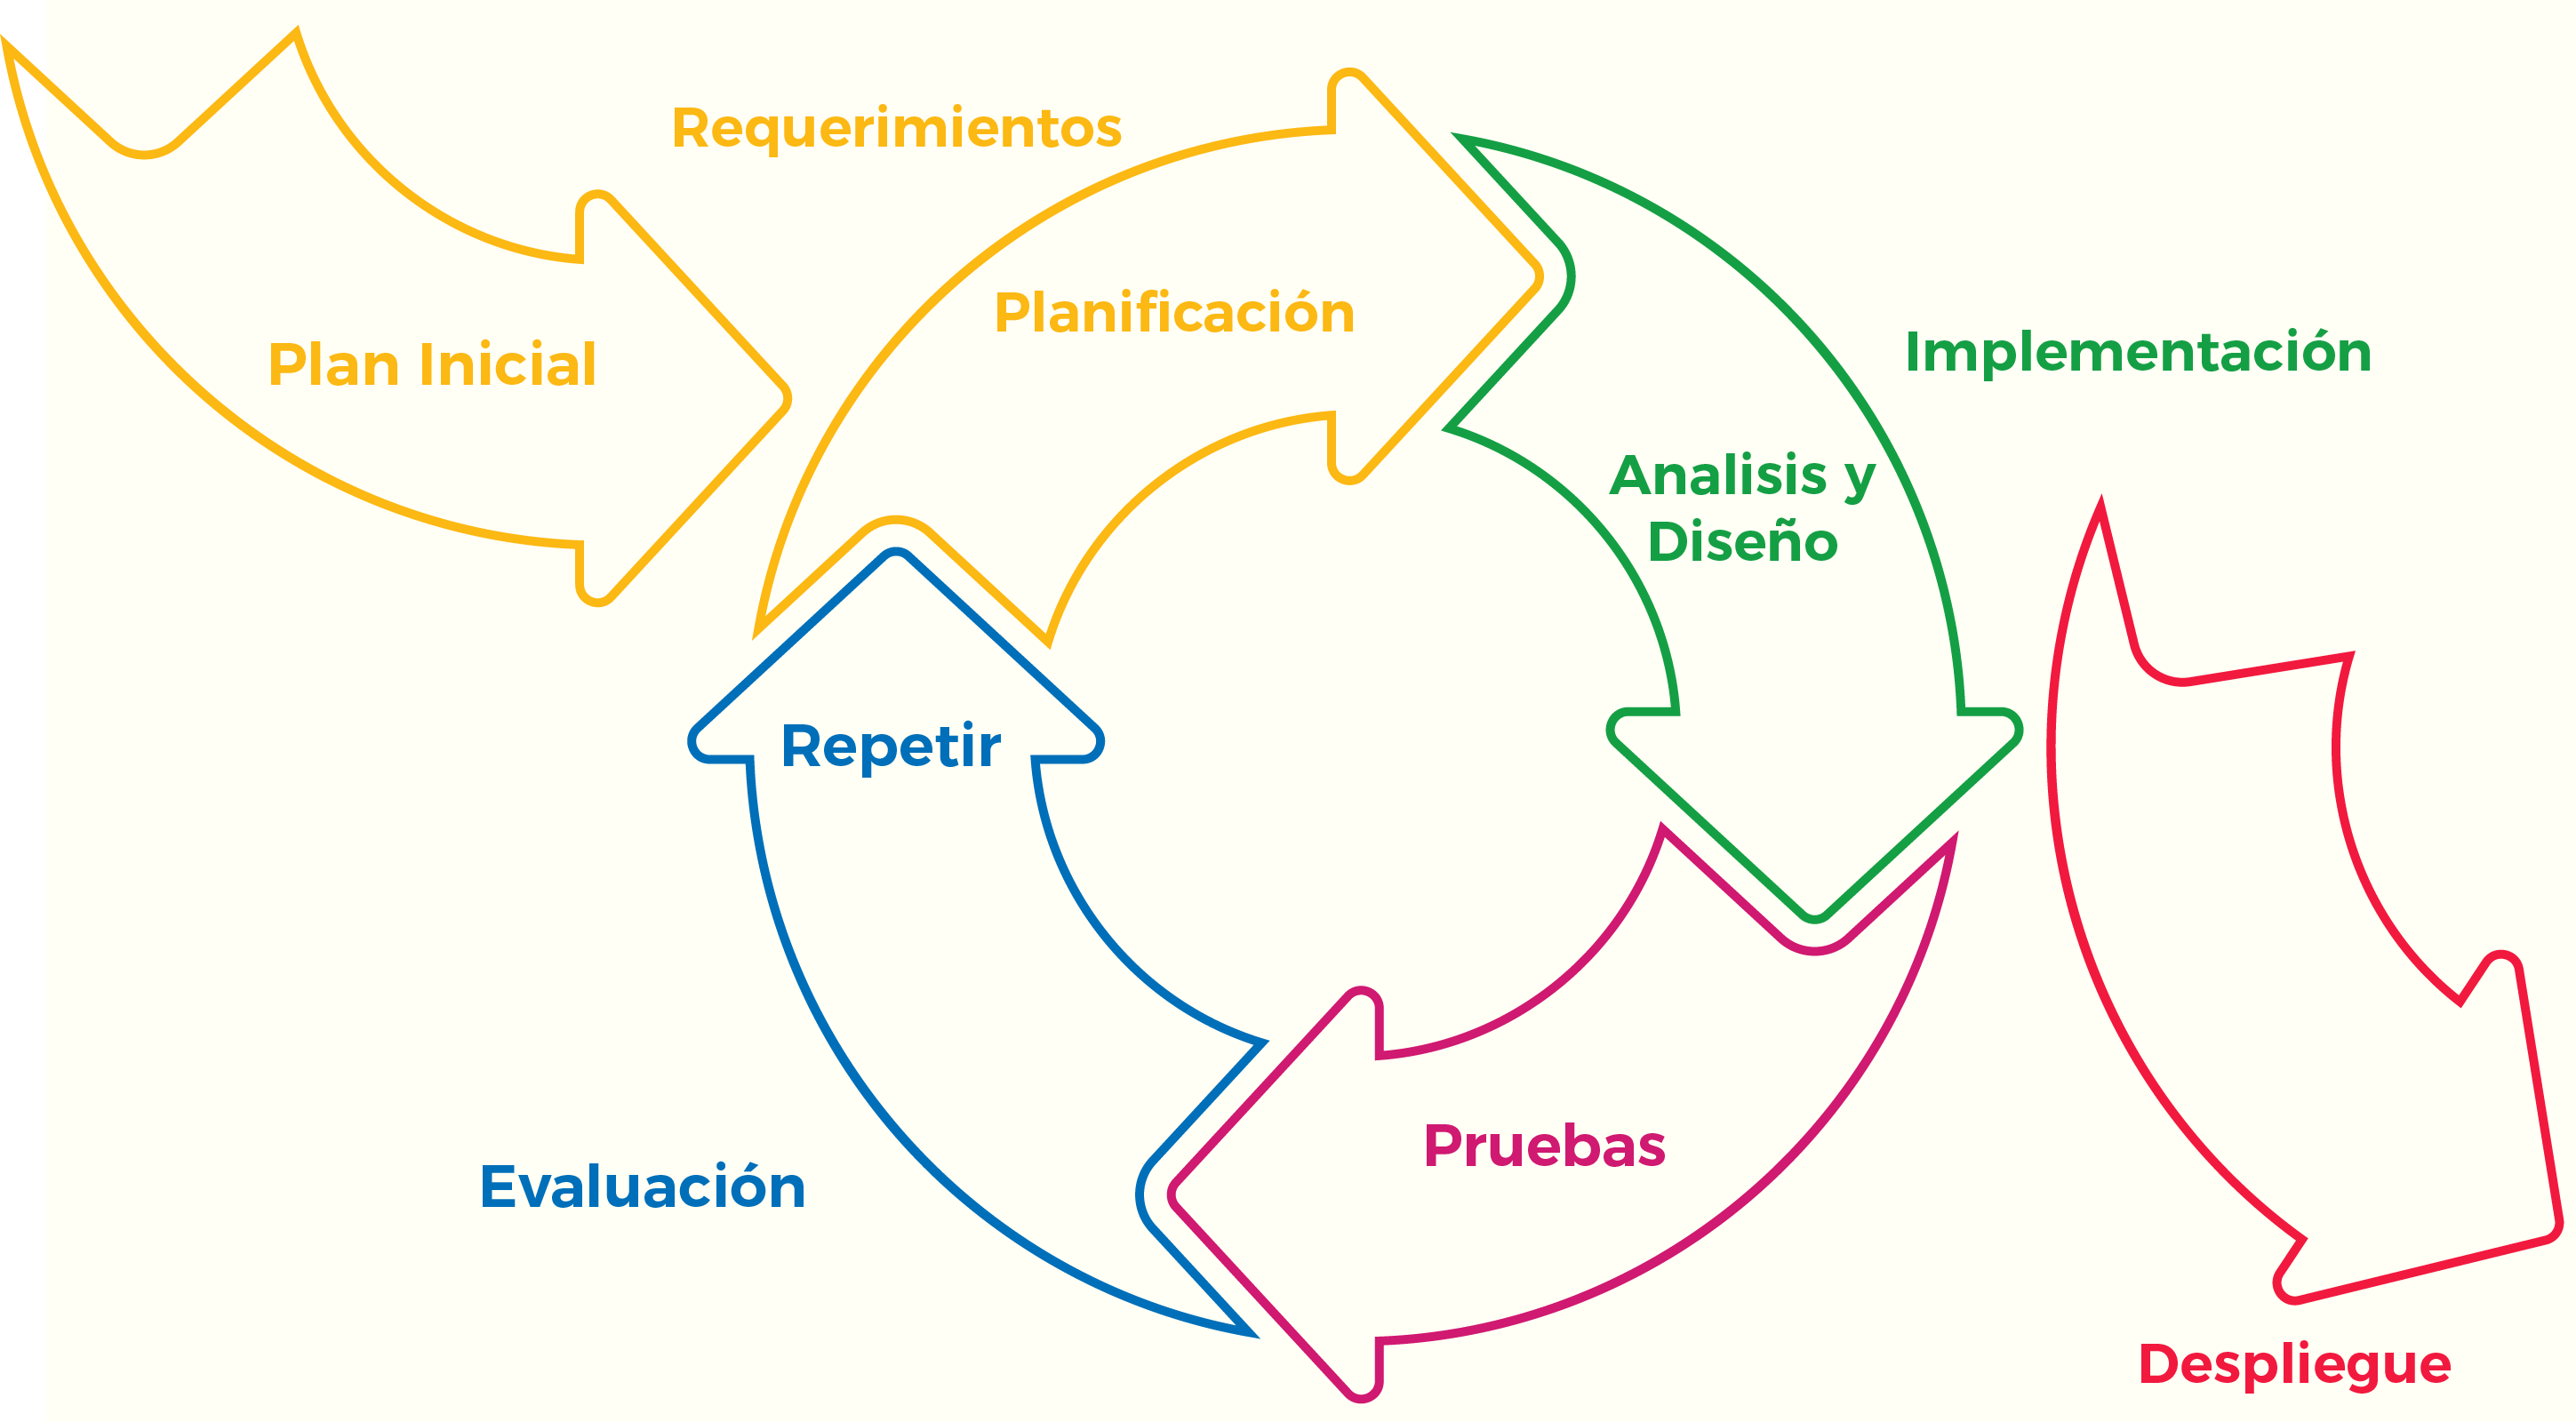
\includegraphics[width=0.9\textwidth]{img/metodoiterativo.png}
    \caption{Metodología de modelo iterativo} \label{fig:metodo}
\end{figure}

Cuando los cambios eran revisados por el tutor, se seguía una dinámica de \textit{Incidencia y parche} en el repositorio principal. Para ello se creaba una incidencia (\textit{issues}) con el tema que se iba a solucionar o añadir en la funcionalidad de la plataforma, y una vez resuelto en local y para cerrarla, se creaba una rama (\textit{branch}) creando parche (\textit{pull request}) para que un desarrollador principal de \textit{Kibotics}, lo aceptará y fusionará con la rama principal y así arreglar la incidencia. Esto se hace para registrar todos los cambios, y comprobarlos antes de que se trabaje directamente en el repositorio



\section{Plan de trabajo}
\label{sec:plan}

El plan de trabajo a seguir para conseguir el objetivo se puede dividir en los siguientes pasos:
\begin{itemize}
    \item \textit{Paso 1}: Aterrizaje en \textit{Kibotics}. Lo primero que hay que hacer es familiarizarse con el entorno con el que se va a trabajar. \textit{Kibotics} es una plataforma web en la que entraremos mas en detalle en el siguiente capitulo 
    \item \textit{Paso 2}: Comienzo de la creación del robot simulado. Comenzaremos por la creación de varios modelos 3D para usarlos en el entorno simulado, son varios diferentes ya que lo original que tiene \textit{LEGO} es poder construir tu robot en base a la tarea que vaya a realizar, con las piezas que incluye el kit. Además de la creación de los ejercicios que lleven a probar las funciones implementadas, para probar su funcionamiento, así como para añadirlos a la plataforma.
    \item \textit{Paso 3}: Desarrollo de las funciones y ejercicios dentro de la aplicación de \textit{Kibotics} para crear una dinámica de trabajo con el nuevo robot.
    \item \textit{Paso 4}: Dar soporte al robot real para poder programarlo en \textit{python} desde el exterior, y la instalación de un server para que pueda recibir código y ejecutarlo en local.\newline
Probar que funciona este envio de programas,con la ejecución de ejercicios programados en el navegador
    \item \textit{Paso 5}: Creación de los \textit{drivers} que hagan de traductor entre lo que creas en la plataforma, y lo que entiende el robot. 
\end{itemize}
% INFRAESTRUCTURA %
%%%%%%%%%%%%%%%%%%%%%%%%%%%%%%%%%%%%%%%%%%%%%%%%%%%%%%%%%%%%%%%%%%%%%%%%%%%%%%%%
%\chapter{Herramientas}
\label{chap:herramientas}
En este capítulo se van a detallar las herramientas y tecnologías utilizadas en el desarrollo de este proyecto principalmente en el ámbito web. Algunas se han elegido por facilidad de uso y otras por necesidad del entorno desarrollado.

\section{Robot Lego Ev3}
\label{sec:caracteristicas} 
Dentro de los robots de \textit{LEGO} el que más versatilidad, además de más potencia de procesamiento y posibilidades en las opciones de creatividad a la hora de crear robots es \textit{LEGO MINDSTORMS Education}\cite{bib:mindstorm} (Pack en el que viene integrado el \textit{LEGO Ev3}) también trae una mayor gama de sensores, por no decir que es uno de los líderes en la educación STEM (siglas en inglés de Ciencias, Tecnología,Ingeniería y Matemática). En el centro de \textit{LEGO MINDSTORMS Education} se encuentra el Bloque EV3, el bloque inteligente programable que controla motores y sensores y además proporciona comunicación inalámbrica.
 \begin{figure}[H]
    \centering
    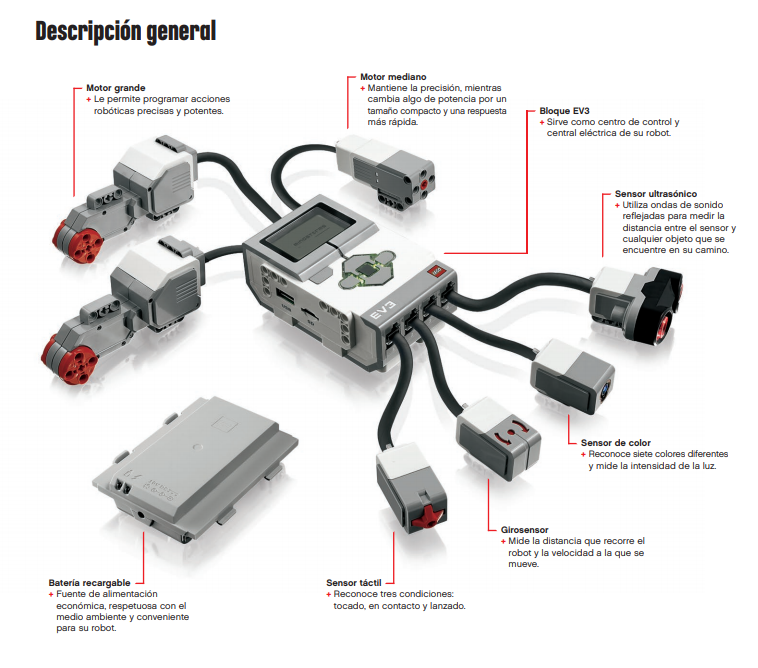
\includegraphics[scale=0.7]{img/partes.png}
    \caption{Conjunto Ev3} \label{fig:partes}
\end{figure}
 Esto quiere decir que las posibilidades a la hora de crear diferentes robots, con diferentes configuraciones de sensores, son prácticamente infinitas. Pero vamos a centrarnos en los casos que más funcionalidad tienen. El robot que más versatilidad presenta a la hora de superar ejercicios, es un robot triciclo, con dos ruedas delanteras y una pivotante trasera. Así que este será nuestro modelo para el robot. Y además, como el \textit{kit de LEGO MINDSTORMS} viene con tres sensores diferentes, crearé tres modelos para integrarlos por separado en la plataforma.

\section{Lenguaje Python}

Python es un lenguaje de programación administrado por la Python Software Foundation.Posee una licencia de código abierto, denominada Python Software Foundation License.Es un lenguaje interpretado, por lo que no se necesita compilar el código fuente para poder ejecutarlo. Esto ofrece ventajas como la rapidez de desarrollo e inconvenientes como una menor velocidad. En ciertos casos, cuando se ejecuta por primera vez un código, se producen unos bytecodes que se guardan en el sistema y que sirven para acelerar la compilación implícita que realiza el intérprete cada vez que se ejecuta el mismo código. 
Este lenguaje nos es muy importante en este proyecto ya que es el lenguaje nativo del robot y en el que van a ir programados los \textit{drivers} para el robot real. 

\section{Lenguaje HTML}

HTML (HyperText Markup Languaje) fue desarrollado en 1991 por Tim Berners-Lee mientras trabajaba en la Organización Europea para la Investigación Nuclear (CERN), y popularizado por el navegador Mosaic desarrollado en NCSA (Raggett, Le Hors y Jacobs, 1999).

Es un lenguaje de marcado que sirve para estructurar una página web. Permite poner etiquetas a diferentes partes de la página para darles la misma apariencia. También tiene tipos de funciones para personalizar el tipo de letra y la forma que tienen en pantalla

Un documento HTML tiene una estructura de árbol  donde la etiqueta html es el elemento raíz y cada nuevo elemento es una rama del anterior. Estas ramas se pueden ir extendiendo sea necesidad del proyecto web.

\begin{lstlisting}[frame=single,breaklines=true, label=Ejemplo de funcionamiento HTTP, caption=Ejemplo de funcionamiento HTTP, captionpos=b]

<!DOCTYPE html>
<html>
  <head>
    <meta charset="utf-8">
    <title>Mi pagina de prueba</title>
  </head>
  <body>
    <img src="images/firefox-icon.png" alt="Mi imagen de prueba">
  </body>
</html>
\end{lstlisting}

HTML5 es la mejora de HTML, establece una serie de nuevos elementos y atributos que reflejan el uso actual de los sitios web modernos, incluye nuevas etiquetas como \texttt{<nav>} que es el bloque de navegación del sitio web. Tiene soporte para \textit{Canvas} y visores para MathML y SVG.\newline

Usare HTML para crear el editor web que se encargará de enviar el código al robot.

\section{Lenguaje JavaScript}
\label{sec:js}
\textit{JavaScript} es un lenguaje de programación interpretado de alto nivel que se encuentra bajo el estándar ECMA Script. Este lenguaje es comúnmente conocido por su uso en los scripts de las páginas web. Es un lenguaje tipado débil y dinámico. Esta diseñado para ser utilizado en páginas Web, actualmente existen otras posibilidades de ejecutar \textit{JavaScript} en todo tipo de aplicaciones haciendo uso de \textit{Nodejs}.\newline
La sintaxis es similar a la utilizada en Java y C++. De esta manera, se facilita el aprendizaje del lenguaje ya que está basado en conceptos ya conocidos por el programador.\newline
Este es el lenguaje en el que estan programados los \textit{drivers} de los robots simulados en la plataforma \textit{Kibotics}. 
% A-FRAME %
\section{Entorno A-Frame}
\label{sec:aframe}
\textit{A-Frame}: \footnote{\url{https://aframe.io/}}  es un entorno de código abierto destinado a crear experiencias de realidad virtual, siendo una de las comunidades creadoras de contenido para realidad virtual más grandes del mundo. Esto se debe a que es un entorno soportado por la mayoria de gafas de VR(\textit{Virtual Reality}) como \textit{OculusRift, HTC Vive o GearsVR}.\newline
\begin{figure}[ht]
    \centering
    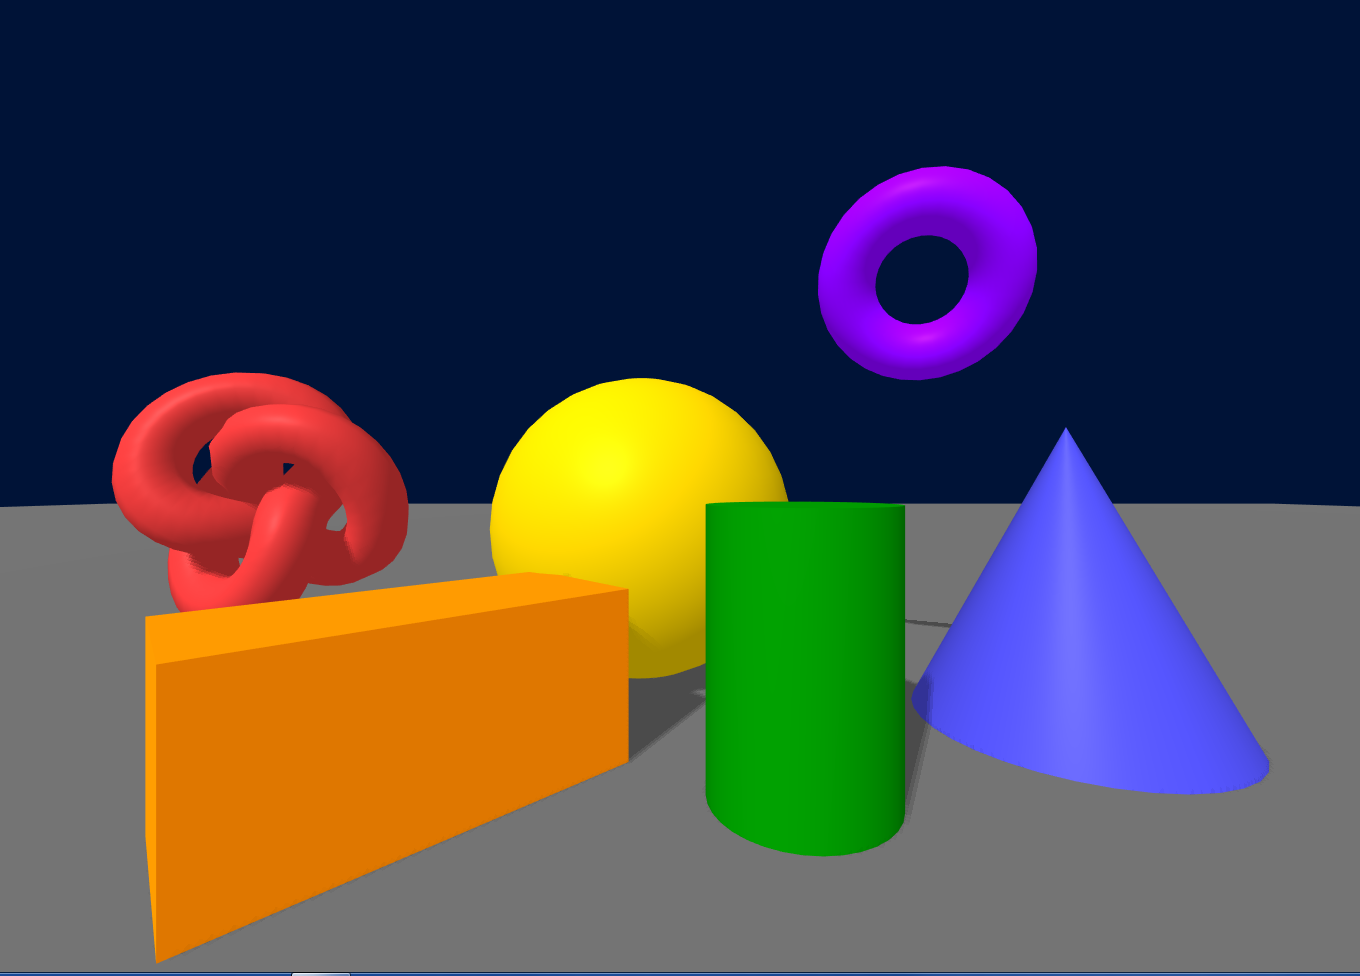
\includegraphics[width=1\textwidth]{img/Aframe.png}
    \caption{Algunos ejemplos de \textit{A-Frame}} 
    \label{fig:A-Frame}
\end{figure}

Esta creado a partir de \textit{HTML} de forma que sea sencillo de leer y comprender. De esta manera es accesible para crear una gran comunidad. \textit{A-Frame} sigue el patrón ECS(entidad-componente-sistema). Se trata de un patrón de desarrollo de juegos basado en el principio de composición sobre herencia. De esta manera, se otorga una mayor flexibilidad en la definición de entidades ya que cada objeto de la escena se corresponde con una entidad y cada entidad,a su vez, está compuesta por uno o más componentes que contienen datos y estado de la entidad. Por tanto, una entidad puede verse modificada en tiempo de ejecución si alguno de los componentes que agrega modifica sus datos.
\\
A-Frame es la base sobre la que esta programado el simulador de la plataforma de \textit{Kibotics}.


% BLENDER %
\section{Editor 3D Blender}
\label{sec:blender}
\textit{Blender} \footnote{\url{https://www.blender.org/}} es un programa libre dedicado al diseño y animación 3D. Mediante una interfaz gráfica permite diseñar objetos, personajes y escenas en tres dimensiones con muy diversas técnicas. Cada uno de los elementos creados pueden ser animados mediante \textit{keyframing} o animación por fotogramas clave. En su origen \textit{Blender} fue distribuido como una herramienta privada explotada por un estudio de animación, pero actualmente se encuentra bajo licencia \textit{GPL} 

    
\begin{figure}[ht]
    \centering
    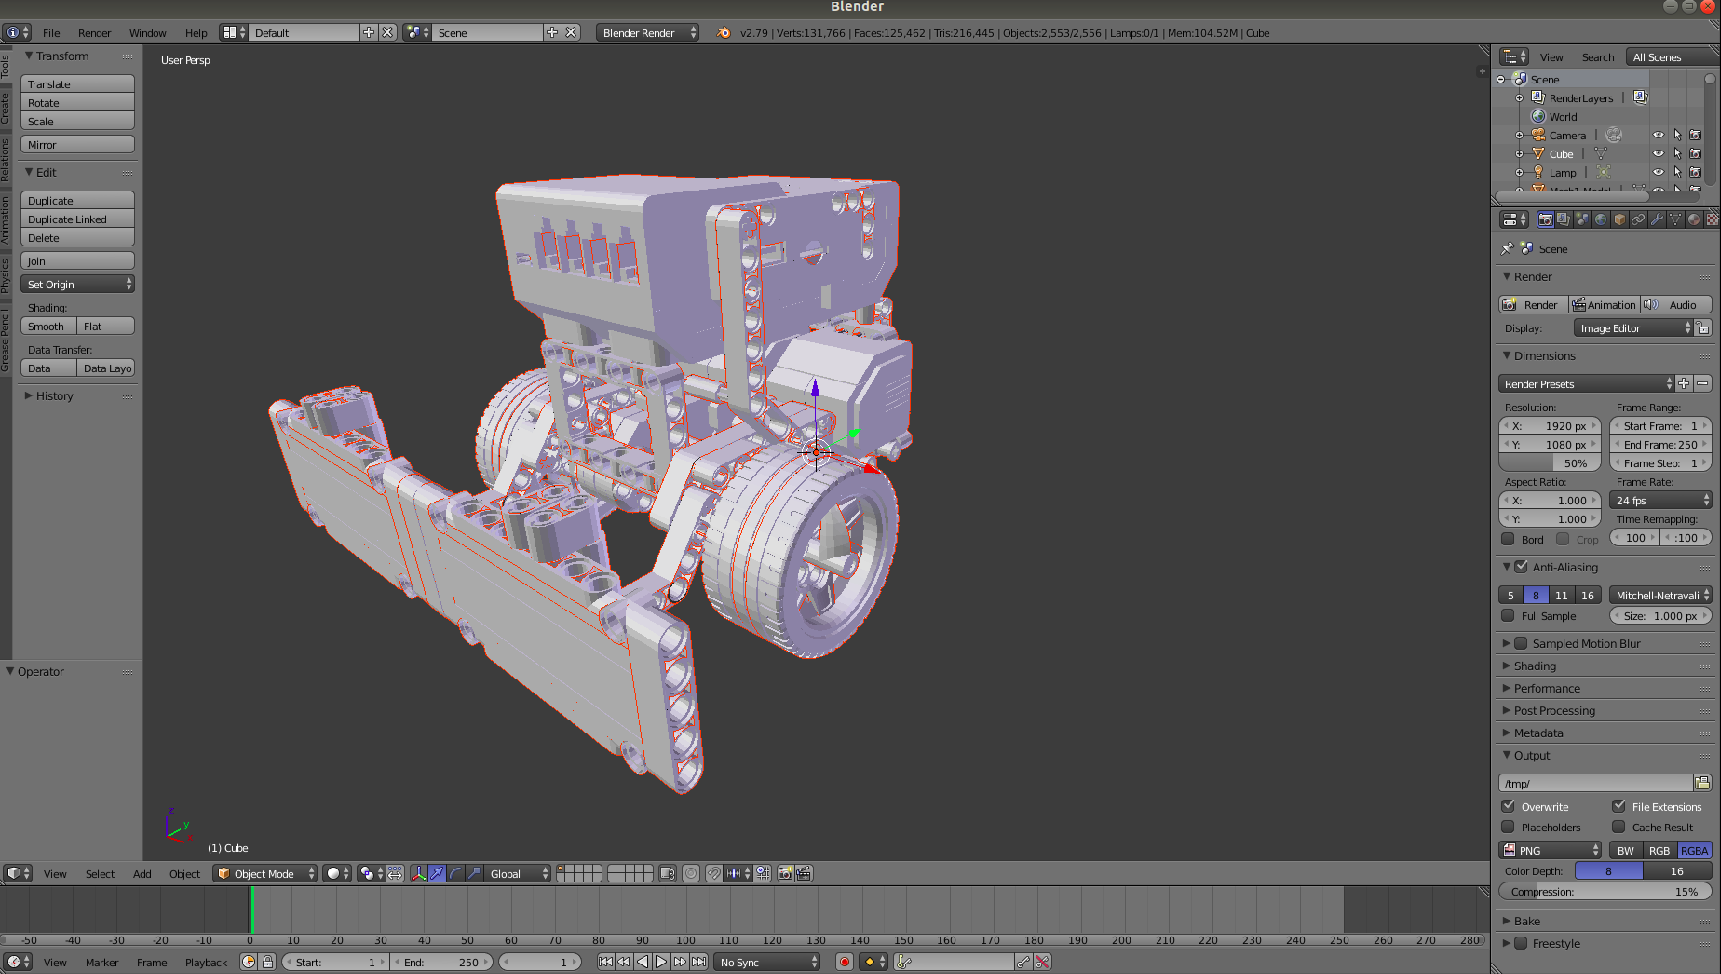
\includegraphics[width=1\textwidth]{img/primermodelo.png}
    \caption{Interfaz gráfica de \textit{Blender}} 
    \label{fig:blender}
\end{figure}

Existe un almacén web desde donde es posible descargarse una gran variedad de modelos y escenarios, además de desarrollar los propios. Una vez desarrollado el modelo o escenario, estos editores exportan el modelo o escenario en formato "gltf", que es un formato soportado por \textit{A-Frame} y estaría listo para insertarlo en el entorno simulado.\newline
Los escenarios y modelos generados por este editor son creados mediante la intersección de líneas, generando los distintos tipos de objetos. Es posible adjuntar una textura o color a cada cara que forma el objeto. Esto lo utilizaré a la hora de crear mis modelos tridimensionales y poder integrarlos en la plataforma \textit{Kibotics}.


% WEBSIM %
\section{Simulador WebSim}

\textit{Websim} es un simulador diseñado para enseñar conceptos básicos de tecnología e iniciar a niños en robótica y programación. 
El simulador hace uso del entorno \textit{A-Frame} y su diseño permite conectar un editor de texto o un editor de bloques para  programar en \textit{JavaScript}, \textit{Blockly} o \textit{Python} y conectar este código con el robot simulado.  En la figura \ref{fig:websim} se puede ver el diseño de \textit{WebSim}.
    

\begin{figure}[H]
    \centering
    \includegraphics[width=1\textwidth]{img/websim.png}
    \caption{Interfaz gráfica de \textit{WebSim}} \label{fig:websim}
\end{figure}

Las características del simulador hacen que los usuarios puedan programar el robot simulado de manera sencilla, ya que solo tengan que acceder a la información que ofrecen los sensores del robot y mandar ordenes a los actuadores. Es decir, que solo tengan que programar la lógica del robot para resolver los ejercicios propuestos. 

El robot consta de sensores simulados con \textit{A-Frame}. Los drivers permiten que el usuario, vía \textit{JavaScript}, pueda acceder a estos y obtener su información. En este entorno disponemos de los siguientes sensores: 

\begin{table}[H]
\caption{Métodos (HAL API) de los sensores del robot.}
\vspace{0.5cm}
\label{tab:tablaSensores}
\resizebox{\textwidth}{!}{%
\begin{tabular}{|c|c|c|ll}
\cline{1-3}
\textbf{Método} & \textbf{Descripción} & \textbf{Salida} &  &  \\ \cline{1-3}
.getDistance() & \begin{tabular}[c]{@{}c@{}}Devuelve la distancia entre el robot\\  y la intersección del raycaster en el centro\end{tabular} & number(metros) &  &  \\ \cline{1-3}
.getDistances() & \begin{tabular}[c]{@{}c@{}}Devuelve la distancia entre el robot y\\ la intersección con cada una de los raycaster\end{tabular} & list number(metros) &  &   \\ \cline{1-3}
.readIR(color) & \begin{tabular}[c]{@{}c@{}}Recorta la imagen, filtra y calcula el centro\\ del objeto con el color pasado como argumento\end{tabular} & number &  &  \\ \cline{1-3}
.getRotation() & \begin{tabular}[c]{@{}c@{}}Retorna un objeto con la orientación \\ del robot en los 3 ejes\end{tabular} & \begin{tabular}[c]{@{}c@{}}\{x:number,\\ y:number,\\ z:number\}\end{tabular} &  &  \\ \cline{1-3}
.getPosition() & Obtiene la posición del robot en la escena & \begin{tabular}[c]{@{}c@{}}\{x:number,\\ y:number,\\ z:number\}\end{tabular} &  &  \\ \cline{1-3}
.getImage() & Devuelve la imagen de la cámara del robot & cv.Mat() &  &  \\ \cline{1-3}
.getObjectColor(color) & \begin{tabular}[c]{@{}c@{}}Devuelve un objeto con la posición del elemento\\ detectado por la cámara del color pasado por parámetro\end{tabular} & \begin{tabular}[c]{@{}c@{}}\{center:{[}x.y{]},\\ area: int\}\end{tabular} &  &  \\ \cline{1-3}
.getObjectColorRGB(valorBajo,valorAlto) & \begin{tabular}[c]{@{}c@{}}Devuelve un objeto con la posición del elemento\\ detectado por la cámara con los valores pasados por parámetro\end{tabular} & \begin{tabular}[c]{@{}c@{}}\{center:{[}x.y{]},\\ area: int\}\end{tabular} &  &  \\ \cline{1-3}
\end{tabular}%
}
\end{table}

Además de sensores, el robot tiene actuadores. Los actuadores se encargan de dar movimiento al robot simulado en \textit{A-Frame}.

En la tabla \ref{tab:tablaMotores} se explican todas las funciones del \textit{HAL API} que hacen referencia a los actuadores.

\begin{table}[H]
  \begin{center}
    \caption{Métodos (HAL API) de los actuadores del robot en \textit{JavaScript}.}
    \vspace{0.5cm}
    \label{tab:tablaMotores}
    \begin{tabular}{|c|c|} 
    \hline
      \textbf{Método} & \textbf{Descripción}\\
      \hline
.setV(integer) & \begin{tabular}[c]{@{}c@{}}Mueve hacia delante o atrás el robot.\\\end{tabular} \\ \hline
.setW(integer) & \begin{tabular}[c]{@{}c@{}}Hace girar al robot.\\\end{tabular} \\ \hline
.move(integer, integer) & \begin{tabular}[c]{@{}c@{}}Mueve el robot hacia delante/atrás y gira al mismo tiempo.\\ \end{tabular} \\ \hline
.getV() & \begin{tabular}[c]{@{}c@{}}Obtener la velocidad lineal configurada en el robot.\\ \end{tabular} \\ \hline
.getW() & \begin{tabular}[c]{@{}c@{}}Obtener la velocidad angular configurada en el robot.\\ \end{tabular} \\ \hline
    \end{tabular}
  \end{center}
\end{table}

Además del \textit{Driver} en \textit{Javascript} para los robots simulados, la plataforma de \textit{Kibotics} ofrece recubrimientos de este HAL API en \textit{Python} y en \textit{Scratch}. Los usuarios programan sus aplicaciones robóticas usando esos interfaces de alto nivel.

\section{Servidor Django}

Django \footnote{\url{https://www.djangoproject.com/es}} un entorno de código abierto escrito en Python, creado en 2005, el cual permite desarrollar un entorno web complejo de una forma rápida y estructurada. Actualmente es mantenido por Django Software Foundation y se encuentra en la versión 3.0, aunque para este proyecto vamos a usar la versión 2.2, que es la que utiliza \textit{Kibotics} actualmente.

Sigue una arquitectura MVC (Modelo – Vista - Controlador), como se observa en la figura.
\begin{itemize}
	\item \textit{Modelo}. Es la representación de la información con la cual el sistema opera, por lo tanto gestiona todos los accesos a dicha información, tanto consultas como actualizaciones, implementando también los privilegios de acceso que se hayan descrito en las especificaciones de la aplicación

	\item \textit{Vista}. Presenta el 'modelo' en un formato adecuado para interactuar (usualmente la interfaz de usuario), por tanto requiere de dicho 'modelo' la información que debe representar como salida.
	
	\item \textit{Controlador}. Responde a eventos e invoca peticiones al 'modelo' cuando se hace alguna solicitud sobre la información.por tanto se podría decir que el 'controlador' hace de intermediario entre la 'vista' y el 'modelo' (.
\end{itemize}
\begin{figure}[h!]
  \centering
    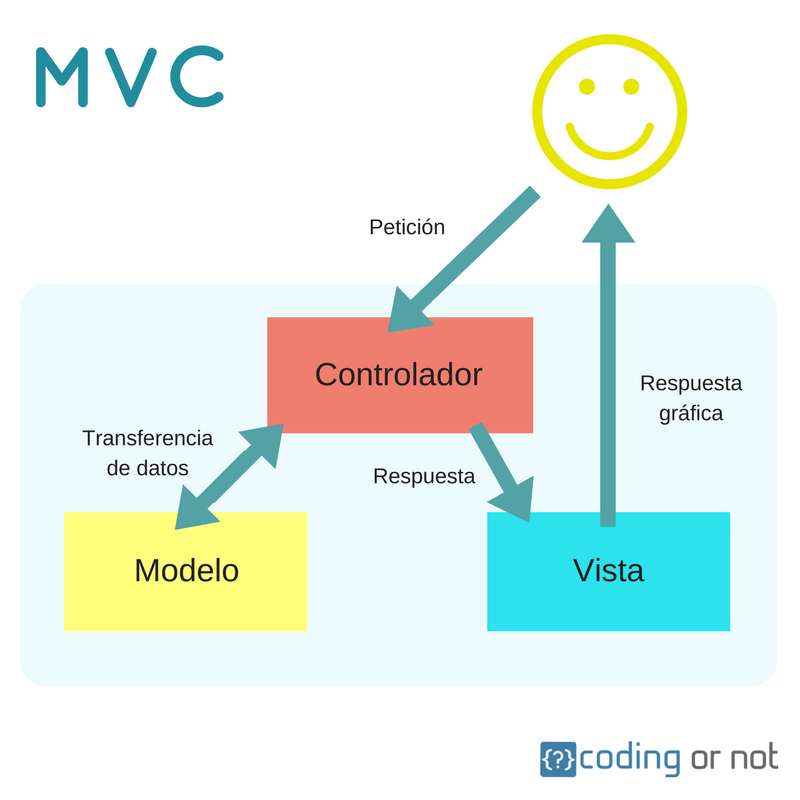
\includegraphics[width=0.6\textwidth]{img/mvc.png}
  \caption{Arquitectura Django}
  \label{Arquitectura Django}
\end{figure}
La meta fundamental de Django es facilitar la creación de sitios web complejos. Django pone énfasis en el re-uso, la conectividad y extensibilidad de componentes, el desarrollo rápido y el principio No te repitas (DRY, del inglés Don't Repeat Yourself). Python es usado en todas las partes del entorno, incluso en configuraciones, archivos, y en los modelos de datos. 


\section{Servidor Flask}

\textit{Flask} \footnote{\url{https://flask.palletsprojects.com/en/1.1.x/}} es un entorno escrito en \textit{Python} y concebido para facilitar el desarrollo de Aplicaciones Web bajo el patrón MVC(Modelo - Vista - Controlador). Se le considera un entrono minimalista porque tiene las herramientas  mínimas necesarias para crear una aplicación web funcional pero si se necesita en algún momento una nueva funcionalidad hay un conjunto muy grande extensiones  que se pueden instalar con \textit{Flask} que le van dotando de funcionalidad.
\begin{figure}[h!]
  \centering
    
\includegraphics[width=0.4\textwidth]{img/flask.png}
  \caption{Logo Flask}
  \label{Flask}
\end{figure}

Usaré \textit{Flask} para instalar un servidor en el robot \textit{LEGO Ev3} que reciba peticiones.

% SOPORTE LEGO EV3 SIMULADO %
%%%%%%%%%%%%%%%%%%%%%%%%%%%%%%%%%%%%%%%%%%%%%%%%%%%%%%%%%%%%%%%%%%%%%%%%%%%%%%%%
%\chapter{Soporte Simulado}
\label{chap:simulado}
Ahora que tenemos definidos cuales van a ser nuestros objetivos, y la infraestructura que vamos a utilizar para llevarlos acabo, en este capítulo, se va a hablar del proceso de integración en la plataforma de la parte simulada del robot. Pero antes de eso se darán unas nociones básicas de las características de este robot, para poder entender, el proceso de desarrollo. 
\section{Características del Lego Ev3}
\label{sec:caracteristicas}
Dentro de los robots de \textit{LEGO} el que mas versatilidad, además de más potencia de procesamiento y posibilidades en las opciones de creatividad a la hora de crear robots es \textit{LEGO MINDSTORMS Education}(Pack en el que viene integrado el \textit{LEGO Ev3}) tambien trae una mayor gama de sensores, por no decir que es uno de los lideres en la educación STEM (siglas en inglés de Ciencias, Tecnología,Ingeniería y Matemática), En el centro de \textit{LEGO MINDSTORMS Education} se encuentra el Bloque EV3, el bloque inteligente programable que controla motores y sensores y además proporciona comunicación inalámbrica como quiera que sea.
 \begin{figure}[H]
    \centering
    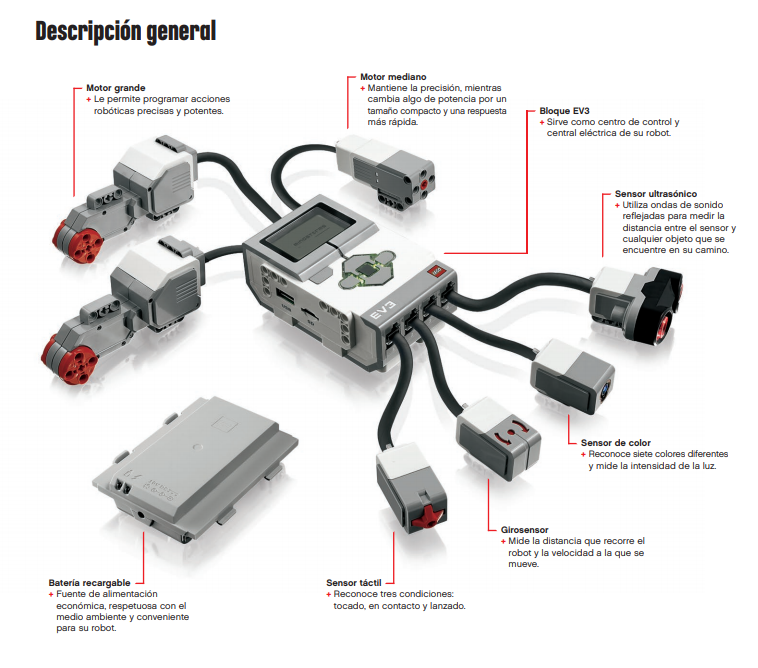
\includegraphics[scale=0.7]{img/partes.png}
    \caption{Conjunto Ev3} \label{fig:partes}
\end{figure}
 Esto quiere decir que las posibilidades a la hora de crear diferentes robots, con diferentes configuraciones de sensores, son prácticamente infinitas. Pero vamos a centrarnos en los casos que mas funcionalidad tienen. El robot que mas versatilidad presenta a la hora de superar ejercicios, es un robot triciclo, con dos ruedas delanteras y una pivotante trasera. Así que este será nuestro modelo para el robot. Y ademas como el \textit{kit de LEGO MINDSTORMS} viene con tres sensores diferentes, crearé tres modelos para integrarlos por separado en la plataforma.
  \begin{figure}[H]
    \centering
    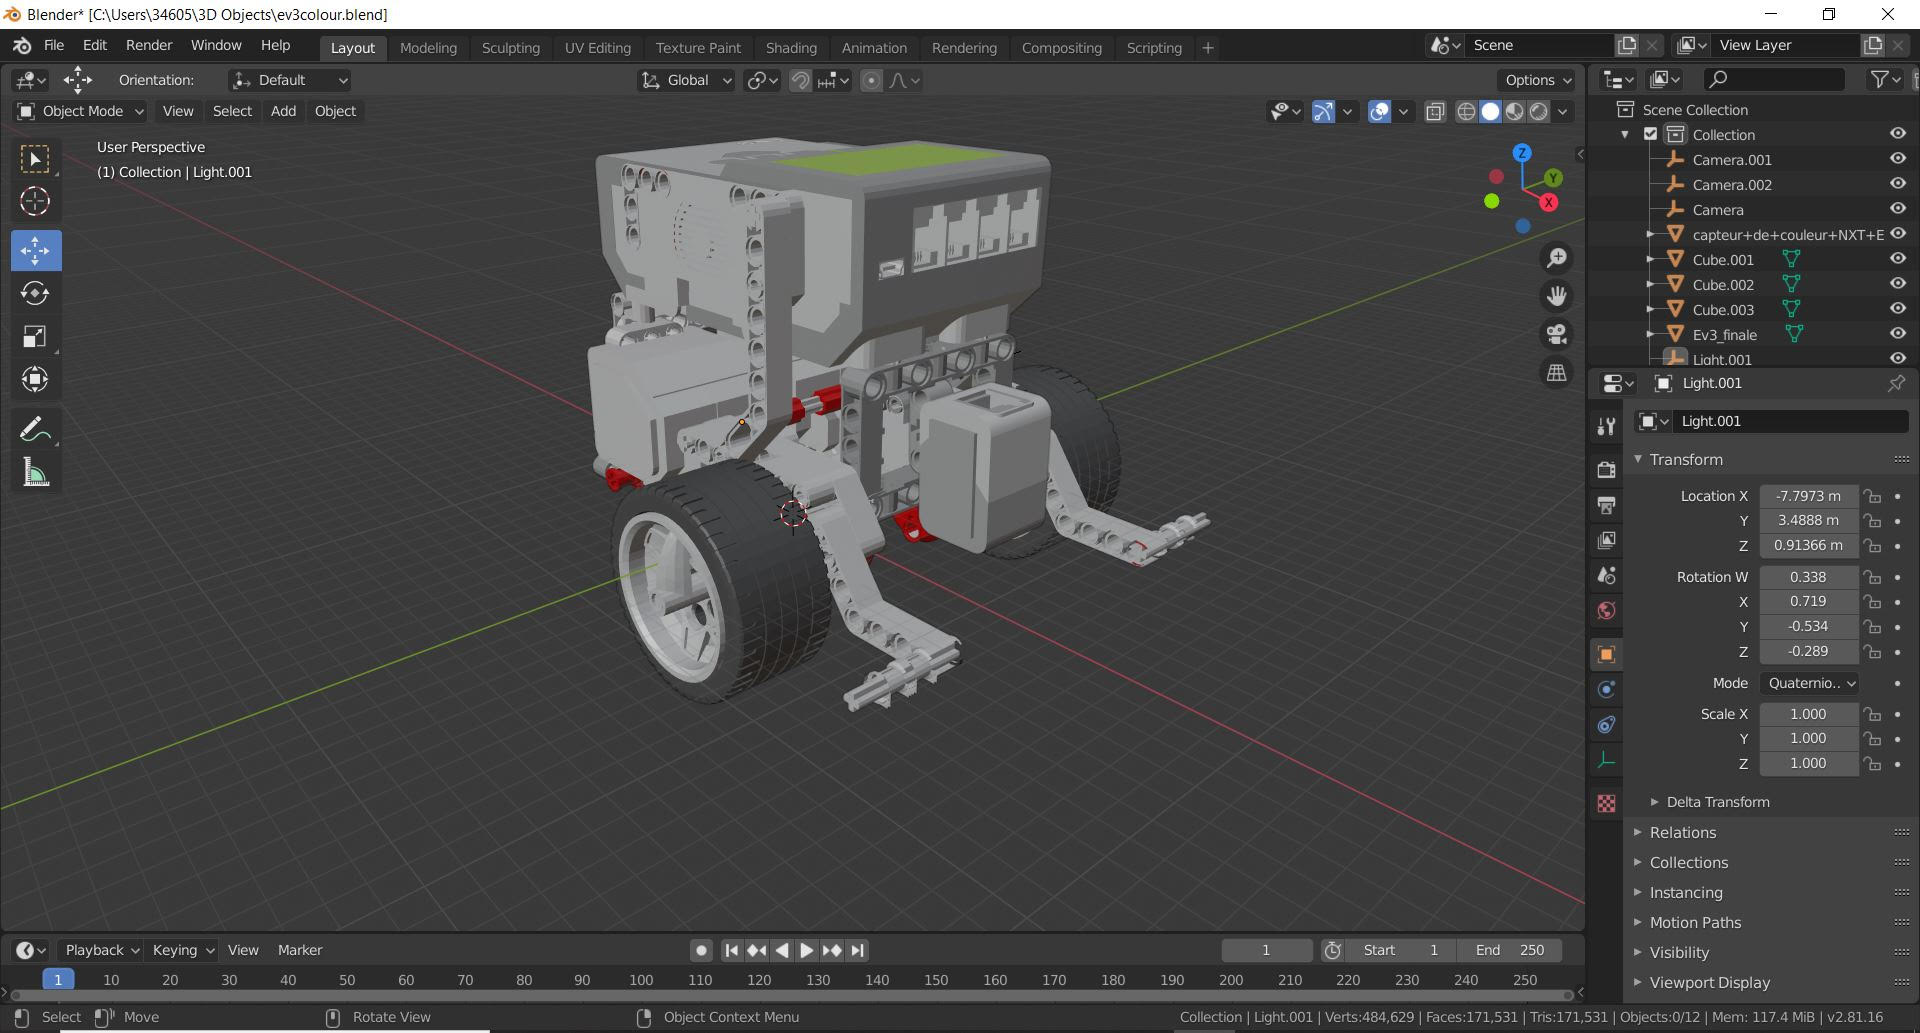
\includegraphics[width=0.7\textwidth]{img/blendercolor.jpg}
    \caption{Robot con sensor de color} \label{fig:color}
\end{figure}
 \begin{figure}[H]
    \centering
    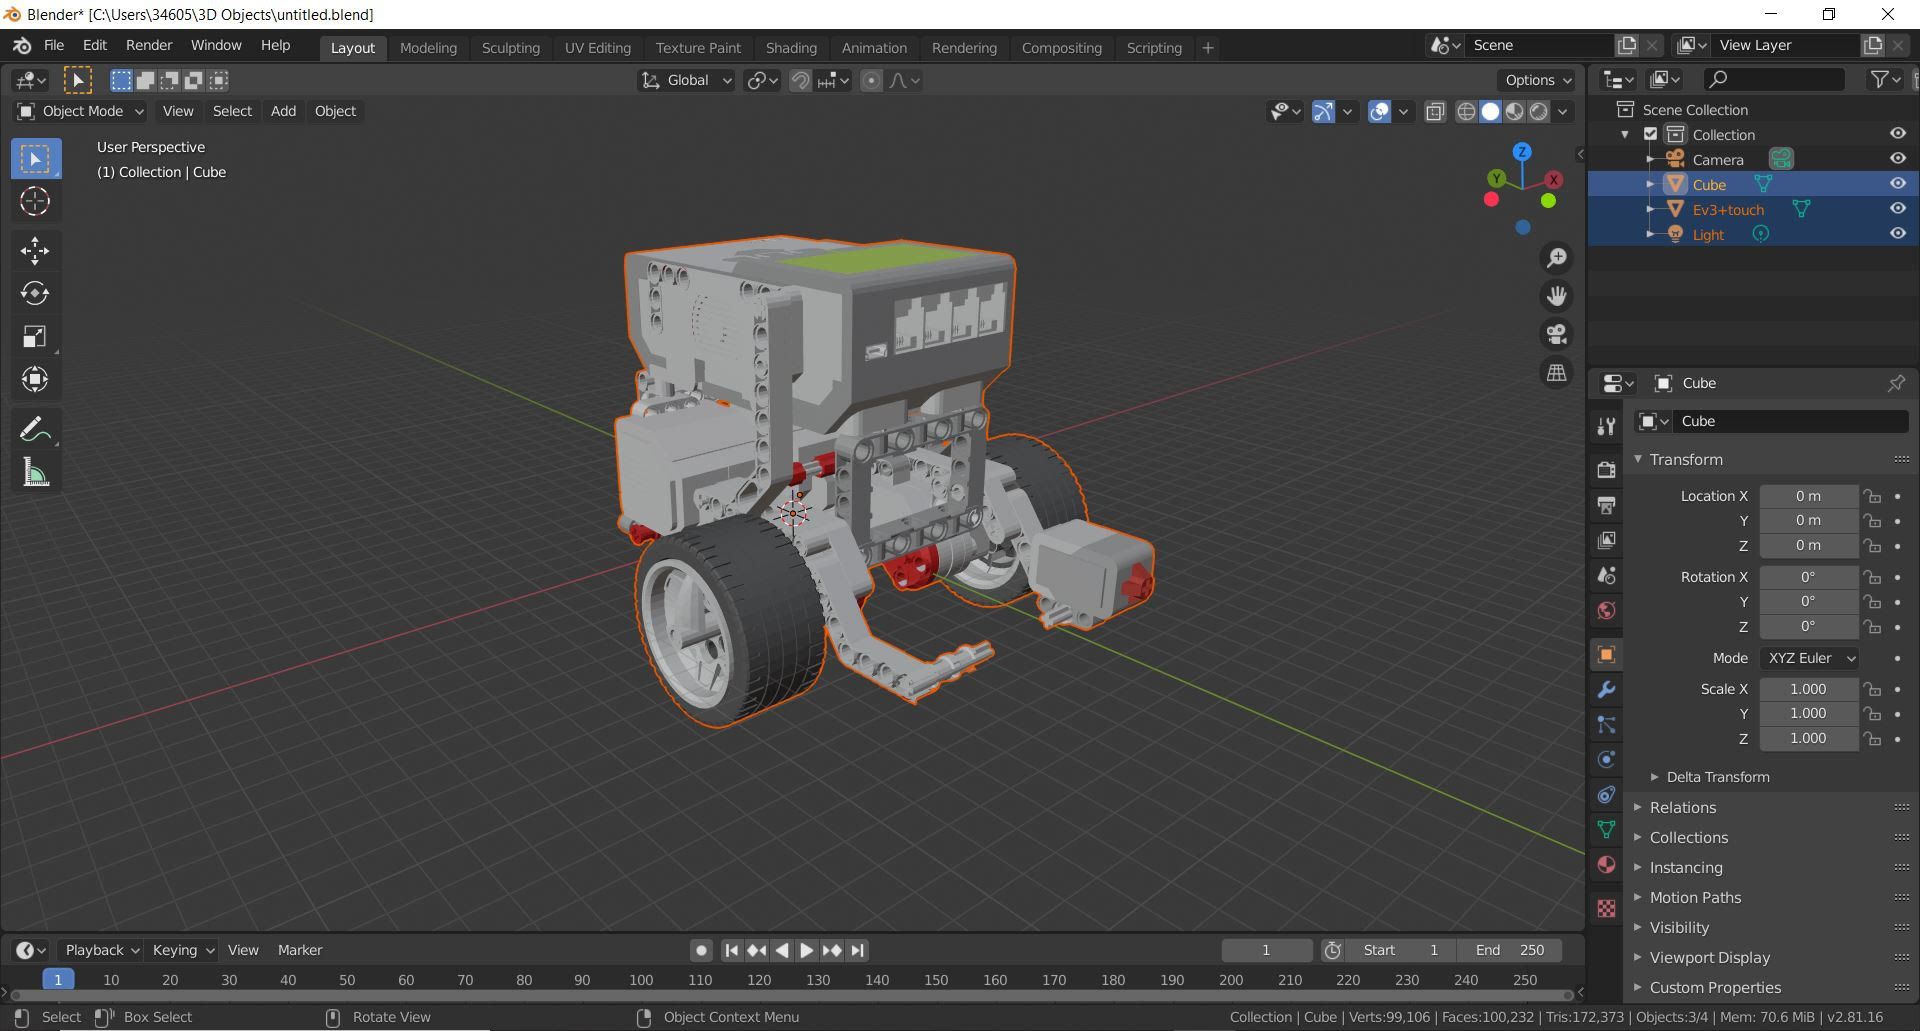
\includegraphics[width=0.7\textwidth]{img/blendertouch.jpg}
    \caption{Robot con sensor tactil} \label{fig:tactil}
\end{figure}
 \begin{figure}[H]
    \centering
    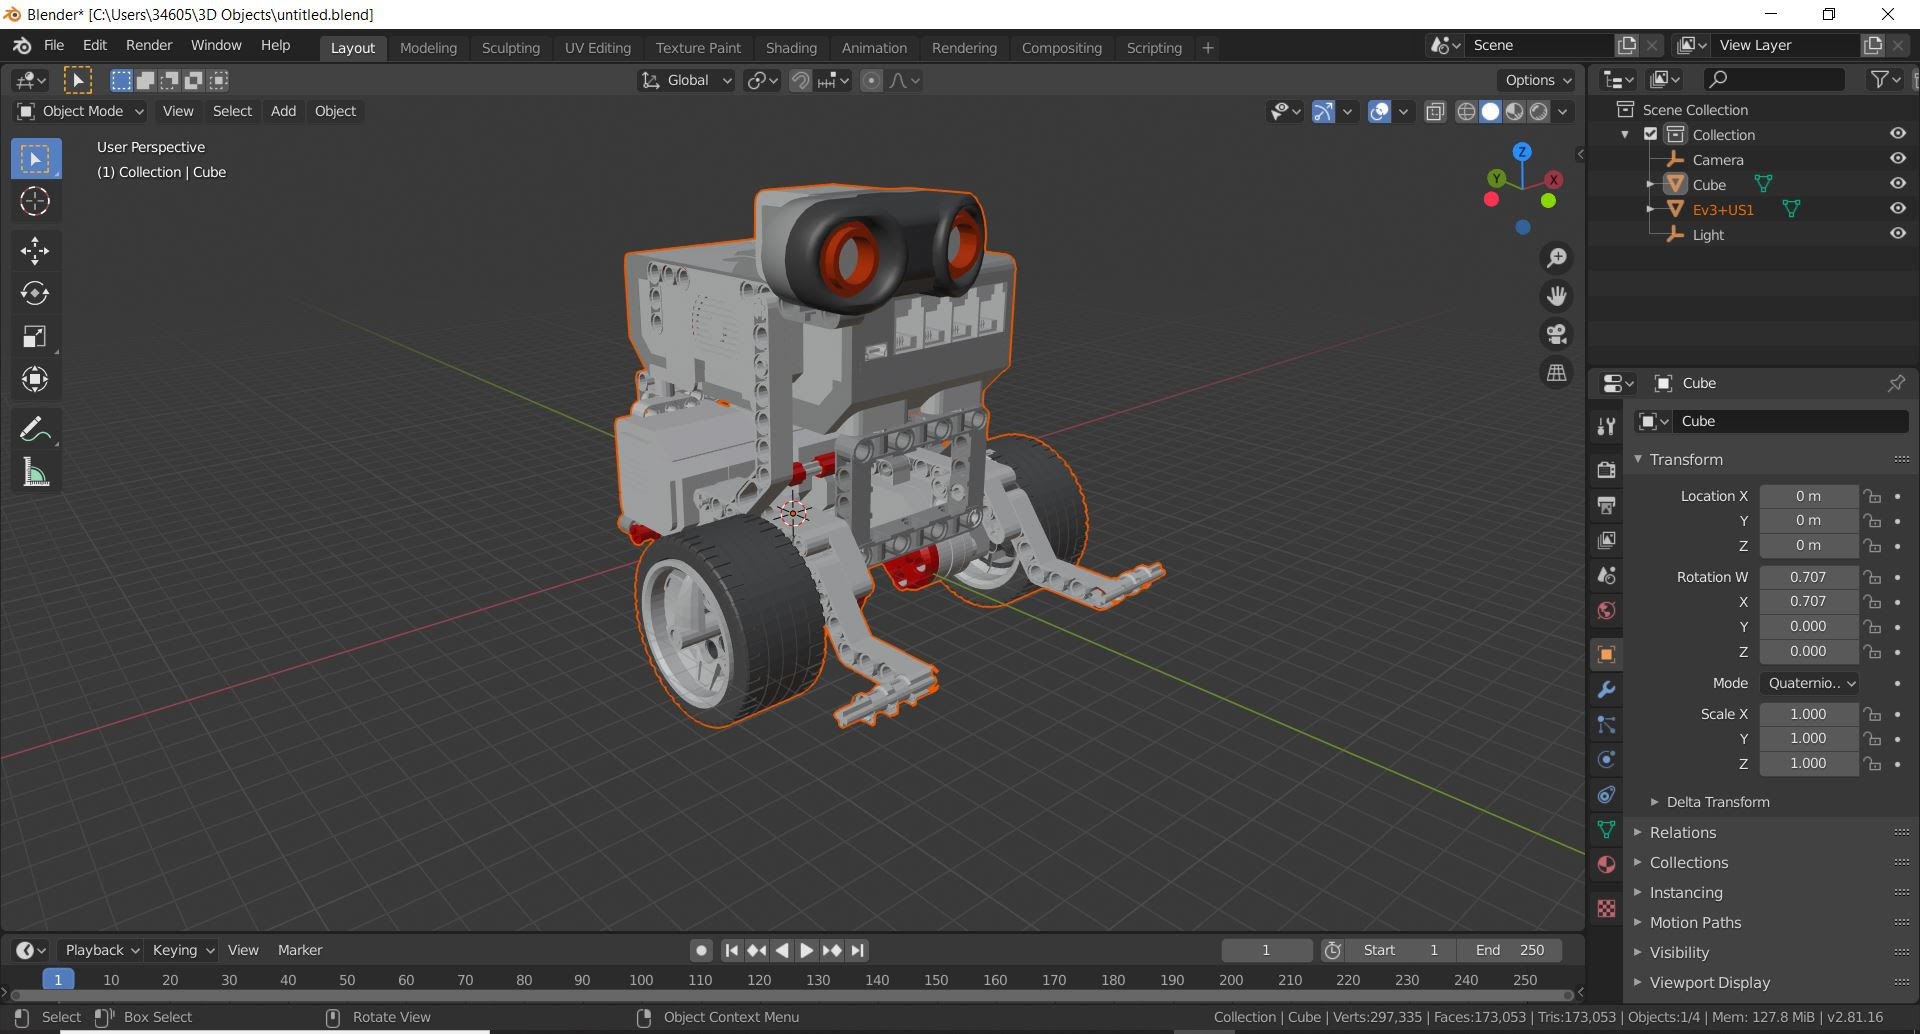
\includegraphics[width=0.7\textwidth]{img/blenderus.jpg}
    \caption{Robot con sensor de ultrasonidos} \label{fig:ultrasonidos}
\end{figure}
Para la tarea del modelaje 3D, he usado el programa de \textit{Blender}. \newline
Ahora que tenemos los tres modelos, voy a dividir el soporte del robot simulado en los diferentes sensores que implementar.
\section{Soporte de sensores}
\label{sec:sensores}

\subsection{Sensor de color}

El primer sensor que vamos a analizar es el sensor de color. El Sensor de color es un sensor digital que puede detectar el color o la intensidad de la luz que ingresa por la pequeña ventana de la cara del sensor. Este sensor puede utilizarse en tres modos diferentes: Modo color, Modo intensidad de la luz reflejada y Modo intensidad de la luz ambiental.\newline
La tasa de muestreo del sensor de color es de 1 kHz.
\begin{wrapfigure}{l}{0.3\linewidth}
    \centering
    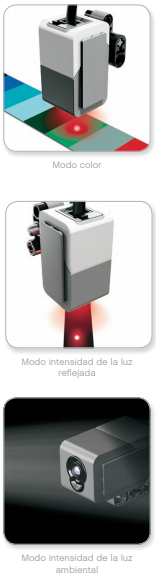
\includegraphics[width=0.6\linewidth]{img/color.png}
    \caption{Sensor color}{{\footnotesize Sensor de color en sus 3 usos}}
    \label{fig:color}
\end{wrapfigure}

\begin{itemize}
\item\textbf{En Modo color}, el Sensor de color reconoce siete colores: negro,
azul, verde, amarillo, rojo, blanco y marrón, además de Sin color.Esta capacidad de diferenciar los colores significa que su robot puede estar programado para clasificar pelotas o bloques de colores, y realizar acciones diferentes con cada color detectado.\newline
Este tipo de acciones, están ya contempladas en la funcionalidad del \textit{HAL API} de \textit{Kibotics}. Aunque en este caso utiliza una camara simulada para comprobar que color esta viendo.\newline
\textit{\textbf{getImage(cameraID)}}: Método que devuelve  \textit{robot}. 
    
    \begin{lstlisting}[language=javascript]
   function getImage(cameraID) {
    /**
     * Returns a screenshot from the robot camera
     */
    if (!cameraID || (this.camerasData.length === 1) || 
    (cameraID > this.camerasData.length - 1)) {
        return this.camerasData[0]['image'];
    } else {
        return this.camerasData[cameraID]['image'];
    }

}
    \end{lstlisting}
\end{itemize}

El \textit{LEGO EV3} no tiene una camara instalada, pero para el robot simulado, es lo mas sencillo de implementar, ya que puede analizar la imagen simulada y sacar el color RGB, para posteriormente dar nombre al color que ve.\newline
\textit{\textbf{getColorRGB()}}: Método que devuelve  \textit{RGB} en tres valores. 
    
    \begin{lstlisting}[language=javascript]
   function getObjectColorRGB(lowval, highval) {
    /**
     * This function filters an object in the scene with a given color, uses OpenCVjs to filter
     * by color and calculates the center of the object.
     *
     * Returns center: CenterX (cx), CenterY (cy) and the area of the object detected in the image.
     */

    if (lowval.length === 3) {
        lowval.push(0);
    }
    if (highval.length === 3) {
        highval.push(255);
    }
    var image = this.getImage();
    var binImg = new cv.Mat();
    var M = cv.Mat.ones(5, 5, cv.CV_8U);
    var anchor = new cv.Point(-1, -1);
    var lowThresh = new cv.Mat(image.rows, image.cols, image.type(), lowval);
    var highThresh = new cv.Mat(image.rows, image.cols, image.type(), highval);
    var contours = new cv.MatVector();
    var hierarchy = new cv.Mat();

    cv.morphologyEx(image, image, cv.MORPH_OPEN, M, anchor, 2,
        cv.BORDER_CONSTANT, cv.morphologyDefaultBorderValue()); // Erosion followed by dilation

    cv.inRange(image, lowThresh, highThresh, binImg);
    cv.findContours(binImg, contours, hierarchy, cv.RETR_CCOMP, cv.CHAIN_APPROX_SIMPLE);
    if (contours.size() > 0) {

        let stored = contours.get(0);
        var objArea = cv.contourArea(stored, false);

        let moments = cv.moments(stored, false);
        var cx = moments.m10 / moments.m00;
        var cy = moments.m01 / moments.m00;

    }
    return {center: [parseInt(cx), parseInt(cy)], area: parseInt(objArea)};
}
    \end{lstlisting}
    
Una vez realizado este paso podemos ponerle un nombre al color, como hace el \textit{LEGO EV3} real.

\begin{itemize}
\item\textbf{En Modo intensidad de la luz reflejada}, el Sensor de color mide la intensidad de la luz que se refleja desde una lámpara emisora de luz color rojo. El sensor utiliza una escala de 0 (muy oscuro) a 100 (muy luminoso). Esto significa que su robot puede estar programado para moverse sobre una superficie blanca hasta detectar una línea negra o para interpretar una tarjeta de identificación con código de color.
Esto en el robot simulado, es diferente, ya que no podemos ver como una magnitud física como es la luz se refleja un objeto, pero este efecto depende del color que se este viendo en la imagen, la luminosidad del color se puede calcular con esta función:

\textit{\textbf{getLightness(valuemin, valuemax)}}: Método que devuelve  \textit{Luminosidad}. 
    
    \begin{lstlisting}[language=javascript]
   function getLightness(valuemin, valuemax) {
    
    let image = this.getObjectColorRGB(valuemin, valuemax);
    let L = ((image.center[0]- image.center[1])/2)*100/255;
    
    /**
     * Returns lightness with a percent
     */
    
    return L.

}
\end{lstlisting}

Esta funcion puede resultar util, para, por ejemplo, poder seguir una linea, cuando haya colores muy similares, o cuando se este utilizando el robot en una mesa o superficie alta, detectar antes, donde esta el borde.

\item\textbf{En Modo intensidad de la luz ambiental}, el Sensor de color mide la intensidad de la luz que ingresa en la ventana desde su entorno, como la luz del sol o el haz de una linterna. El sensor utiliza una escala de 0 (muy oscuro) a 100 (muy luminoso). Esta funcionalidad, no puede ser implementada en la plataforma, ya que no tenemos un foco de luz que se puede analizar, ni tampoco una magnitud dentro del entorno que represente la luz.

\end{itemize}

\subsection{Sensor de ultrasonido}

El Sensor ultrasónico es un sensor digital que puede medir la
distancia a un objeto que se encuentra frente a él. Para hacerlo,
envía ondas de sonido de alta frecuencia y mide cuánto tarda el
sonido en reflejarse de vuelta al sensor. La frecuencia de sonido
es demasiado alta para el oído humano.
La distancia a un objeto puede medirse en pulgadas o centímetros.
Esto le permite programar su robot para que se detenga a una
distancia determinada de una pared.
Al utilizar unidades en centímetros, la distancia detectable es entre
3 y 250 centímetros (con una exactitud de +/- 1 centímetro). Al utilizar
unidades en pulgadas, la distancia detectable es entre 1 y 99
pulgadas (con una exactitud de +/- 0,394 pulgadas). Un valor de
255 centímetros o 100 pulgadas significa que el sensor no puede
detectar ningún objeto frente a él.\newline
\begin{wrapfigure}{r}{0.5\linewidth}
    \centering
    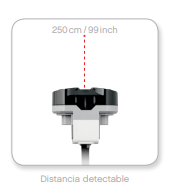
\includegraphics[width=0.5\linewidth]{img/ultrasonidos.png}
    \caption{Sensor de ultrasonidos}
    \label{fig:ultrasonido}
\end{wrapfigure}
En \textit{Kibotics} la implementación que hay para las distancias es  usar un \textit{RayCaster}. Que es equivalente a poner láseres apuntando hacia todas direcciones por delante del robot de estaa forma:


\textit{\textbf{Funciones que calculan la distancia}}: Método que devuelve  un unico valor con la distancia mas corta. 

 \begin{lstlisting}[language=javascript]
function getDistance() {
    /**
     * This function returns the distance for the raycaster in the center of the arc of rays.
     */
    var distances = this.getDistances();

    if (distances[13] !== 10 || distances[14] !== 10 || distances[15] !== 10 || distances[16] !== 10 || distances[17] !== 10) {
        let distance0 = 100;
        let distance1 = 100;
        let distance2 = 100;
        let distance3 = 100;
        let distance4 = 100;
        if (distances[13] !== 10) {
            distance0 = distances[13];
        }
        if (distances[14] !== 10) {
            distance1 = distances[14];
        }
        if (distances[15] !== 10) {
            distance2 = distances[15];
        }
        if (distances[16] !== 10) {
            distance3 = distances[16];
        }
        if (distances[17] !== 10) {
            distance4 = distances[17];
        }
        let min_distances = [distance0, distance1, distance2, distance3, distance4];
        Array.min = function (array) {
            return Math.min.apply(Math, array);
        };
        return Array.min(min_distances);
    } else {
        return 10;
    }
}

function getDistances() {
    /**
     * This function returns an array with all the distances detected by the rays.
     */
    var distances = [];
    for (var i = 0; i <= 31; i++) {
        distances.push(10);
    }
    var groups = ["center", "right", "left"];
    for (i = 0; i < groups.length; i++) {
        this.distanceArray[groups[i]].forEach((obj) => {
            if (typeof obj.d != "undefined") {
                distances[obj.id] = obj.d;
            }
        });
    }
    return distances;
}
\end{lstlisting}


\section{Nuevos ejercicios individuales}
\label{sec:escenarios}

Se han incorporado nuevos escenarios a \textit{WebSim} que dan la posibilidad de realizar nuevos ejercicios y mejorar los ya disponibles. En esta sección se explicarán los nuevos ejercicios desarrollados con un solo \textit{robot} en escena y sus soluciones en \textit{Scratch}.

\subsection{Sigue-líneas visión}
    Este ejercicio consiste en seguir una línea blanca en el suelo sobre fondo negro haciendo uso de la cámara del \textit{robot}, que recoge las imágenes y las filtra para poder seguirla.
    
    Se ha mejorado el escenario cambiando la textura del suelo a una creada con la trazada del circuito de Interlagos de Fórmula 1. Se ha realizado con un programa de diseño gráfico (\textit{Photoshop}) y, debido a su peso computacional, se ha reducido posteriormente su tamaño para aliviar los tiempos de carga. 
    
    \begin{figure}[H]
    \centering
    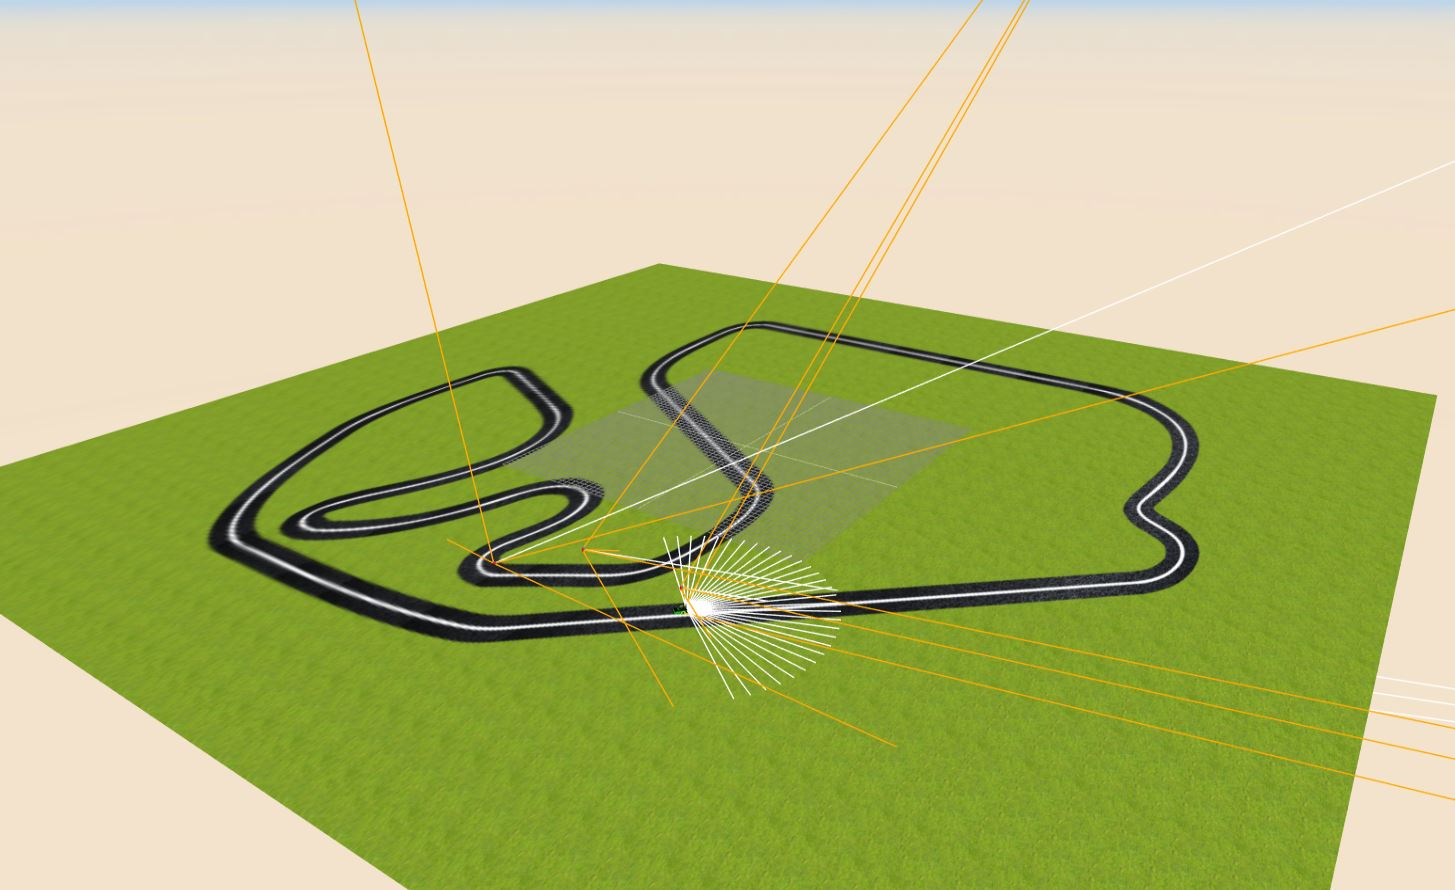
\includegraphics[scale=0.4]{img/pibot_vision.JPG}
    \caption{Escenario para el ejercicio \textit{piBot} sigue-líneas con cámara} \label{fig:siguelineavision}
    \end{figure}
    
        \begin{figure}[H]
    \centering
    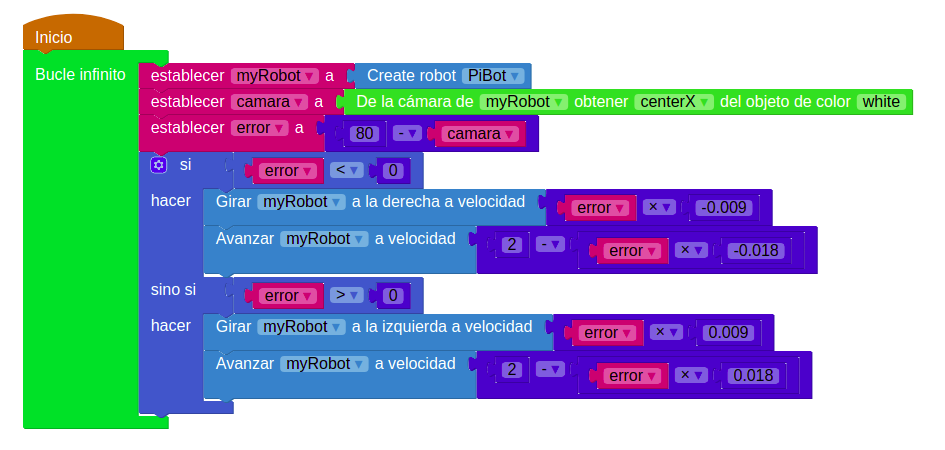
\includegraphics[scale=0.5]{img/siguelineasvisioncodigo.png}
    \caption{Solución en \textit{Scratch} para el ejercicio sigue-líneas visión} 
    \label{fig:visionSolution}
    \end{figure}
    
    En esta solución\footnote{\url{https://youtu.be/fRq__W_BETk}} se comanda velocidad lineal al robot y utiliza el bloque que obtiene el centro del eje X de los objetos blancos. Según el valor obtenido, se gira el \textit{robot} en un sentido u otro.
    
\subsection{Sigue-líneas infrarrojos}
     Este ejercicio consiste en seguir una línea negra en el suelo sobre fondo blanco haciendo uso de los sensores infrarrojos del \textit{robot} que apuntan hacia abajo. 
     
    Tiene un recorrido similar a sigue-líneas visión, pero con fondo blanco y recorrido negro para facilitar la implementación de código en el robot real y que no haya que realizar modificaciones. Para que funcionara correctamente ha sido necesario añadir el color blanco a \textit{undestandedColors} para realizar el filtro y poder pasar ``\textit{white}'' como atributo a la función \textit{getObjectColor()}.
    
    \begin{figure}[H]
    \centering
    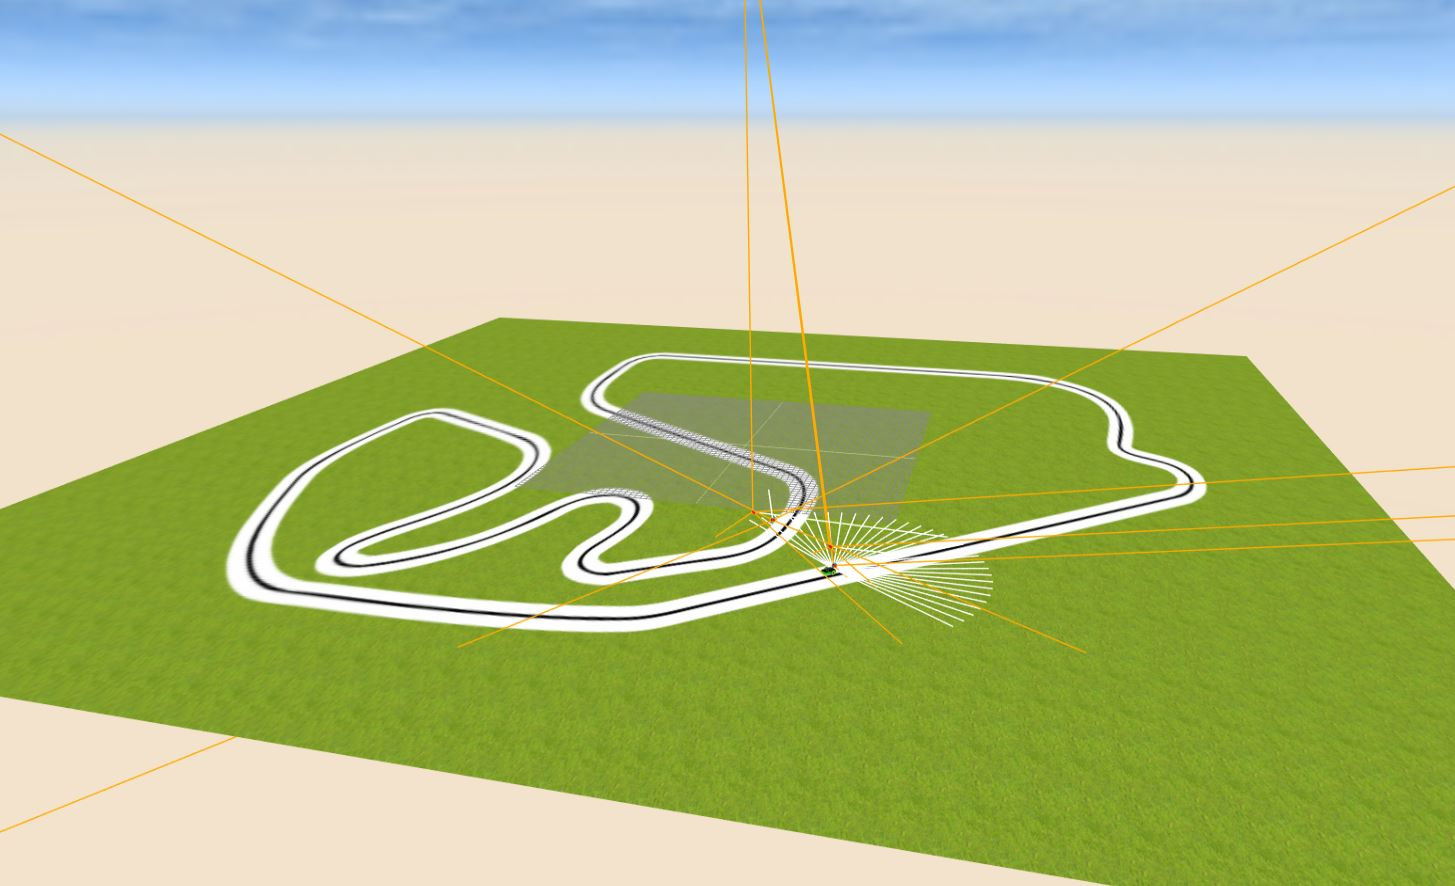
\includegraphics[scale=0.3]{img/siguelineas_ir.JPG}
    \caption{Escenario para el ejercicio para el \textit{robot piBot} sigue-líneas infrarrojos} \label{fig:siguelineasIR}
    \end{figure}
    
           \begin{figure}[H]
    \centering
    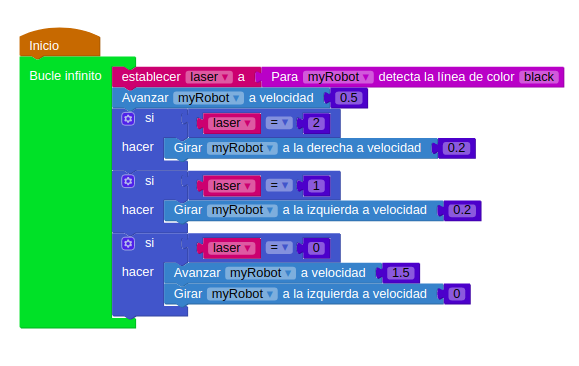
\includegraphics[scale=0.6]{img/siguelineaIRcodigo.png}
    \caption{Solución en \textit{Scratch} para el ejercicio sigue-líneas infrarrojos} 
    \label{fig:irSolution}
    \end{figure}
    
    En esta solución\footnote{\url{https://youtu.be/d4HETtPmahA}} se comanda una velocidad lineal y se obtienen los valores de los sensores infrarrojos del \textit{robot} y se comanda una velocidad angular en función de dónde detecte la línea.
    
\subsection{Choca-gira}
\label{subsec:chocagira}
En este ejercicio hay programar al \textit{robot} para que avance recto mientras no haya obstáculos haciendo uso del sensor de ultra-sonidos. Si encuentra un obstáculo, tiene que detenerse, retroceder un poco, girar un ángulo aleatorio y reemprender la marcha.

Escenario creado en \textit{Blender} con un aspecto similar a su análogo en el simulador \textit{Gazebo}. Para ello se han adaptado la mayor parte de las estructuras que dispone el escenario original para su integración en \textit{WebSim}. 

    \begin{figure}[H]
    \centering
    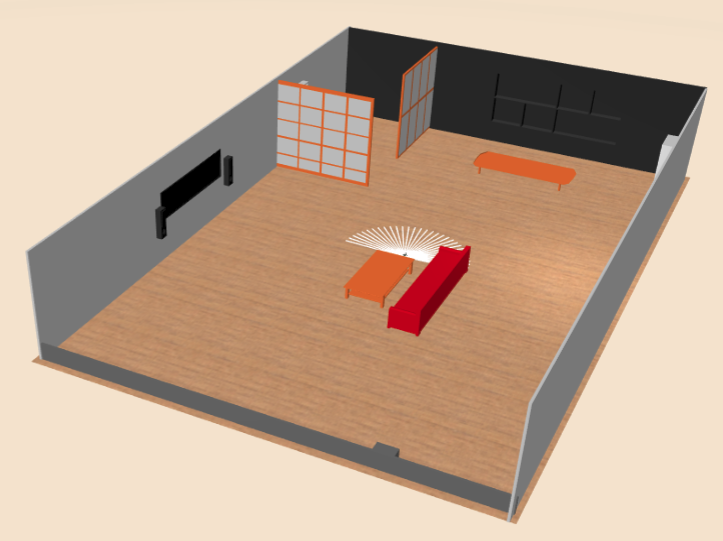
\includegraphics[scale=0.5]{img/bump&go.png}
    \caption{Escenario para el ejercicio choca-gira} \label{fig:chocagira}
    \end{figure}
    \begin{figure}[H]
    \centering
    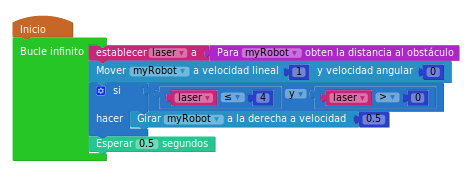
\includegraphics[scale=0.75]{img/chocagiracodigo.png}
    \caption{Solución en \textit{Scratch} para el ejercicio choca-gira} 
    \label{fig:chocagiraSolution}
    \end{figure}
    En esta solución\footnote{\url{https://youtu.be/lXL3lTbgp_E}} se obtienen los valores del sensor de ultra-sonidos y se comanda una velocidad lineal. Si encuentra un obstáculo se gira a la derecha durante 0.5 segundos.
    
\subsection{Sigue-pelota}
\label{subsec:pelota}

Este ejercicio consiste en seguir una pelota en movimiento. Hay que emplear las imágenes obtenidas por el \textit{robot} y programar la lógica de control que permita seguir la pelota.

Se ha realizado dos escenarios distintos, uno para \textit{PiBot} y otro para \textit{drone}.
Ambos disponen de una pelota de color negro, que debe ser seguida usando la cámara del \textit{robot}, a la que se le ha dado movimiento a través de primitivas de \textit{A-Frame}. En la figura \ref{fig:secuenciaDrone} se puede ver una secuencia con la animación de una pelota y en el siguiente código se muestra el archivo de configuración de este ejercicio, que incluye esa animación de \textit{A-Frame}:\\

\begin{lstlisting}[language=json]
{
  "robot": {
    "model":"../assets/models/drone_animation.gltf",
    "scale": "0.5 0.5 0.5",
    "position":"12 1 25",
    "rotation": "0 50 0"
  },
  "gravity": 0,
  "ground": "../assets/textures/escenarioLiso.png",
  "sky": "../assets/textures/sky.png",
  "secondaryCamera": "4 20 30",
  "cameraRobot":"0 0.03 -0.01",
  "objects":[
        {
      "type": "a-sphere",
      "id":"redBall",
      "position": "4 15 20",
      "color": "#000000",
      "radius": "1.5",
      "animation":"property: position; from: 4 15 20 ;to: 0 15 -20; dir: alternate; dur: 10000; loop: true",
      "animation__2":"property: position; from: 0 15 -20 ;to: 0 2 -20 ; delay: 10000; dir: alternate; dur: 10000; loop: true",
      "animation__3":"property: position; from: 0 2 -20 ;to: 4 2 20 ; delay: 20000; dir: alternate; dur: 10000; loop: true",
      "animation__4":"property: position; from: 4 2 20 ;to: 4 15 20; delay: 30000; dir: alternate; dur: 10000; loop: true",
      "animation__5":"property: position; from: 4 15 20 ;to: -10 15 10; delay: 40000; dir: alternate; dur: 10000; loop: true",
      "animation__6":"property: position; from: -10 15 10 ;to: 20 8 -30; delay: 50000; dir: alternate; dur: 10000; loop: true"
      }
      ]
}
\end{lstlisting} 


 Haciendo especial mención al campo \textit{objects}, en el que se crea una pelota negra con la animación indicada en todos los campos \textit{animation} y genera el siguiente elemento en \textit{HTML}, que incluye en el \textit{DOM}:

\begin{lstlisting}[language=html]
<a-sphere id="blackBall" position="12 1 25" color="#000000" radius="1.5" 
    animation="property: position; from: 4 15 20 ;to: 0 15 -20; dir: alternate; dur: 10000; loop: true"
    animation__2="property: position; from: 0 15 -20 ;to: 0 2 -20 ; delay: 10000; dir: alternate; dur: 10000; loop: true" 
    animation__3="property: position; from: 0 2 -20 ;to: 4 2 20 ; delay: 20000; dir: alternate; dur: 10000; loop: true" 
    animation__4="property: position; from: 4 2 20 ;to: 4 15 20; delay: 30000; dir: alternate; dur: 10000; loop: true" 
    animation__5= "property: position; from: 4 15 20 ;to: -10 15 10; delay: 40000; dir: alternate; dur: 10000; loop: true" 
    animation__6="property: position; from: -10 15 10 ;to: 20 8 -30; delay: 50000; dir: alternate; dur: 10000; loop: true">
</a-sphere>
\end{lstlisting}


\begin{figure}[H]
\begin{subfigure}[t]{0.3\textwidth}
  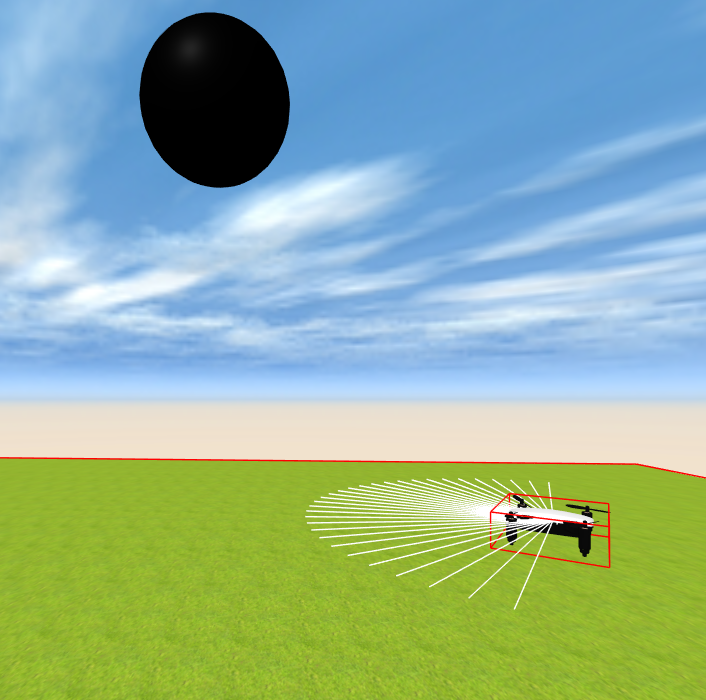
\includegraphics[width=4cm, height=4cm]{img/followBallTello12.png}
\label{fig:figure2_2}
\end{subfigure}\hfill
\begin{subfigure}[t]{0.3\textwidth}
    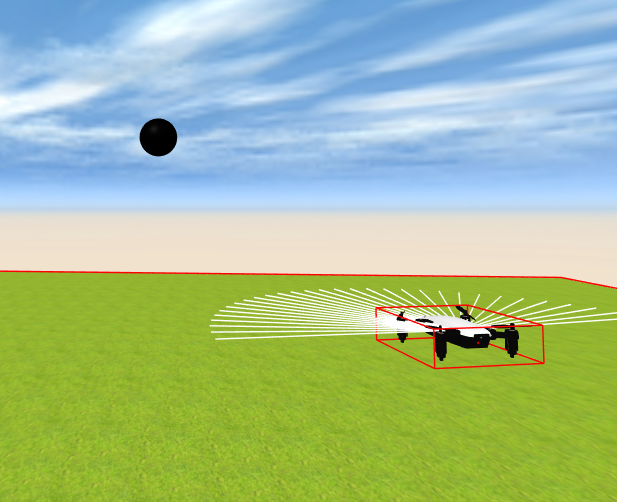
\includegraphics[width=4cm, height=4cm]{img/followBallTello22.png}
\label{fig:figure2_3}
\end{subfigure}\hfill
\begin{subfigure}[t]{0.3\textwidth}
    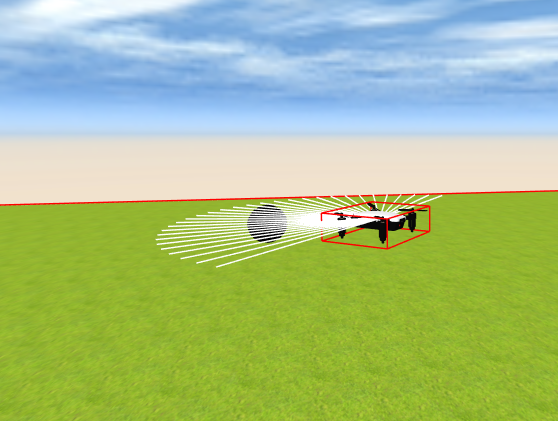
\includegraphics[width=4cm, height=4cm]{img/followBallTello32.png}
\label{fig:figure2_4}
\end{subfigure}
\begin{subfigure}[t]{0.3\textwidth}
    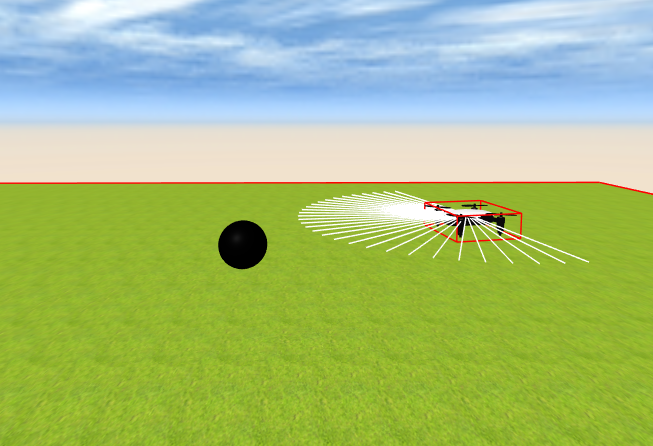
\includegraphics[width=4cm, height=4cm]{img/followBallTello42.png}
\label{fig:figure2_6}
\end{subfigure}\hfill
\begin{subfigure}[t]{0.3\textwidth}
    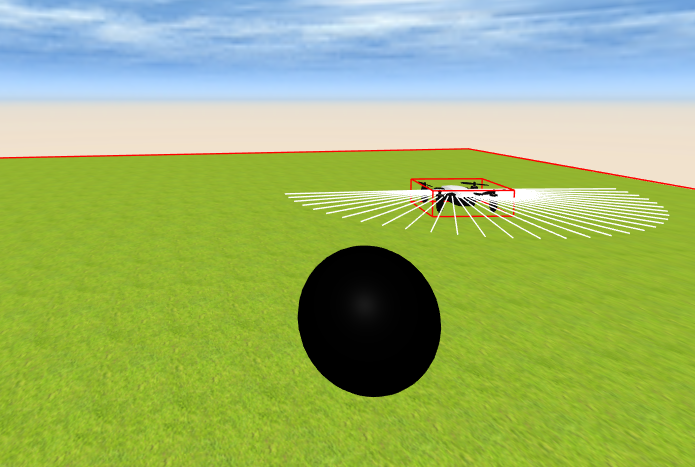
\includegraphics[width=4cm, height=4cm]{img/followBallTello52.png}
\label{fig:figure2_7}
\end{subfigure}\hfill
\begin{subfigure}[t]{0.3\textwidth}
    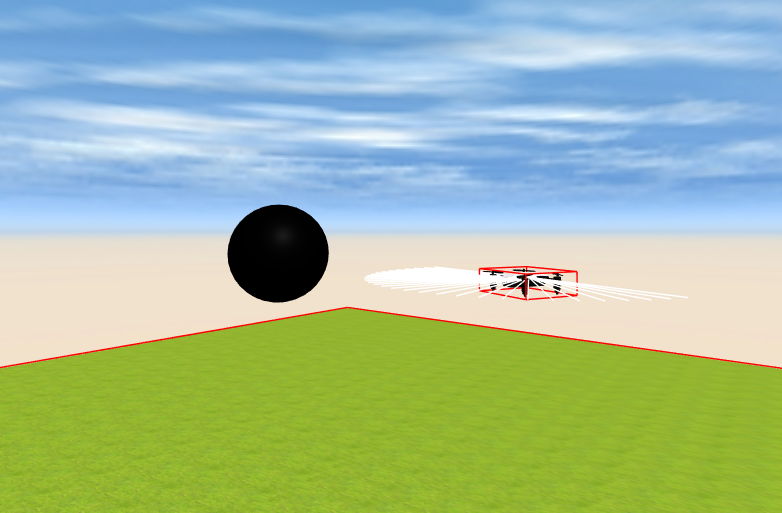
\includegraphics[width=4cm, height=4cm]{img/followBallTello62.png}
\label{fig:figure2_8}
\end{subfigure}

\caption{Secuencia del ejercicio \textit{drone} sigue-pelota}
\label{fig:secuenciaDrone}
\end{figure}


    \begin{figure}[h]
    \centering
    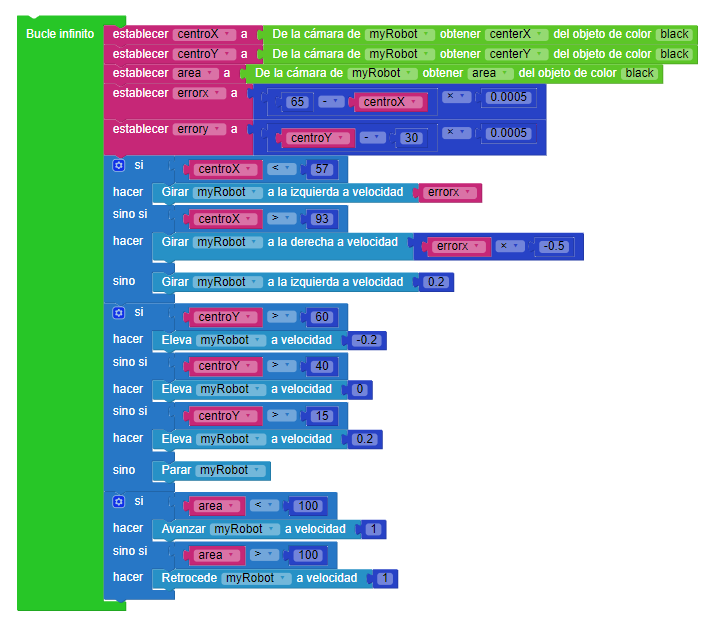
\includegraphics[scale=0.9]{img/siguepelotacodigo.png}
    \caption{Solución en \textit{Scratch} para el ejercicio sigue pelota drone} 
    \label{fig:pelotaSolution}
    \end{figure}
    La solución de este ejercicio\footnote{\url{https://youtu.be/XQrNaWxRg7U}} se ha realizado obteniendo toda la información que aporta la cámara, tanto la posición del objeto en el eje X e Y de la imagen como su área. Según los valores obtenidos se comandan distintas velocidades angulares y lineales. 
\subsection{Atraviesa-bosque}
\label{subsec:atraviesabosque}
Ejercicio basado en atravesar un pasillo con diversos objetos que hay que esquivar. El sensor necesario es el infrarrojos para detectar en que posición se encuentra cada uno de los obstáculos. El escenario y los obstáculos se han creado con primitivas de \textit{A-Frame}.

    \begin{figure}[H]
    \centering
    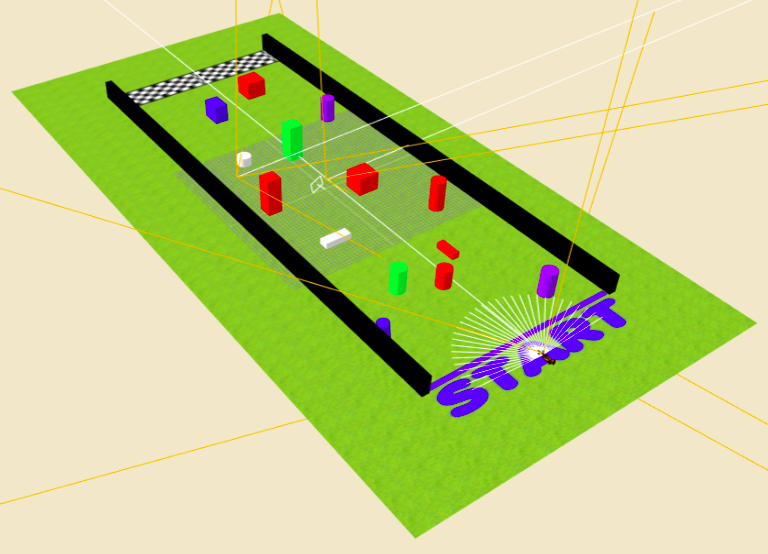
\includegraphics[scale=0.45]{img/atraviesabosque-indiv.png}
    \caption{Escenario para el ejercicio atraviesa bosque} 
    \label{fig:atraviesaBosqueind}
    \end{figure}

    \begin{figure}[H]
    \centering
    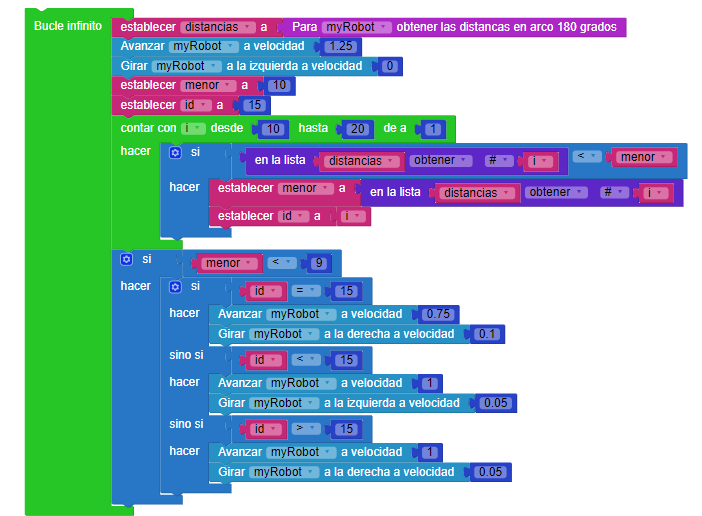
\includegraphics[scale=0.6]{img/atraviesaBosqueCodigo.png}
    \caption{Solución en \textit{Scratch} para el ejercicio atraviesa bosque} 
    \label{fig:bosqueSolution}
    \end{figure}
    
    En esta solución\footnote{\url{https://youtu.be/z3n47wWHDFc}} se obtienen todos los valores que devuelve el sensor de ultra-sonidos y, según donde detecte el obstáculo, gira en un sentido u otro.

\subsection{Cuadrado con drone}
Este ejercicio consiste en comandar velocidades al \textit{drone} para dibujar un cuadrado con el movimiento del \textit{robot}.

    \begin{figure}[H]
        \centering
        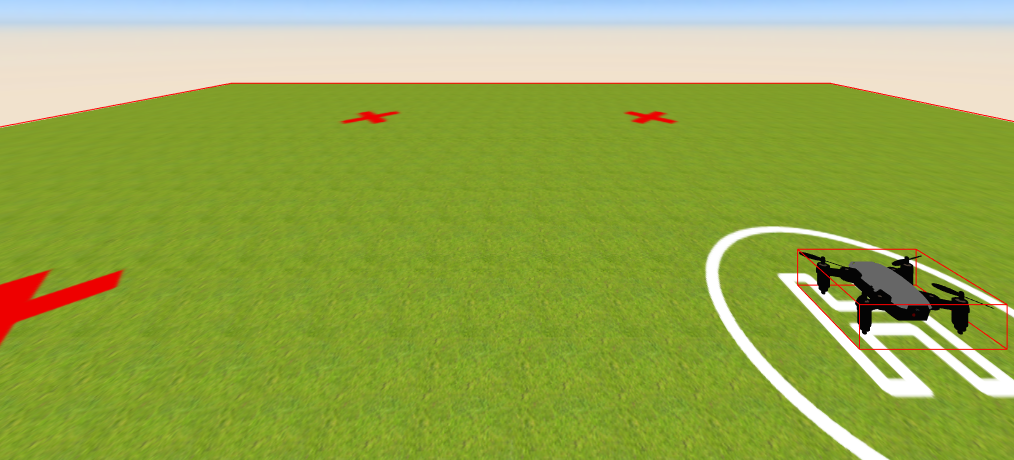
\includegraphics[scale=0.4]{img/cuadradoDrone.png}
        \caption{Escenario de WebSim para el ejercicio drone cuadrado} 
        \label{fig:droneCuadrado}
    \end{figure}

    \begin{figure}[H]
    \centering
    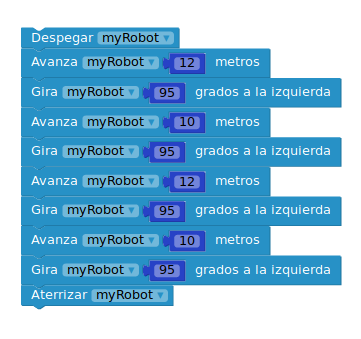
\includegraphics[scale=0.5]{img/tellocuadradocodigo.png}
    \caption{Solución en \textit{Scratch} para el ejercicio cuadrado drone} 
    \label{fig:cuadradoSolution}
    \end{figure}
    Su solución\footnote{\url{https://www.youtube.com/watch?v=XjQNhNCkOJA}} consiste en avanzar los metros necesarios para llegar a la cruz y, cuando se ha completado el desplazamiento, girar 90 grados aproximadamente para así ``dibujar'' un cuadrado repitiendo este proceso.
    
\section{Ejercicios competitivos}
\label{sec:competitive}
Uno de los objetivos de este proyecto era añadir ejercicios competitivos a \textit{Kibotics} sobre el simulador \textit{WebSim}. Se hace especial mención a ellos debido a que son completamente diferentes al resto de los ya creados. Este tipo de ejercicios aumenta el valor de la plataforma ya que da la posibilidad de programar dos robots y ponerlos a funcionar en el mismo escenario simultáneamente, pudiendo entender la programación como un juego en el que se premia al que aporte la mejor solución.

\subsection{Arquitectura de cómputo}
\label{subsec:arquitectura}
En este tipo de ejercicios hay dos robots en una misma escena y cada uno de ellos se puede programar con un código distinto. Para su implementación e integración en \textit{Kibotics} se ha extendido el módulo \textit{brains} y se han incorporado dos aplicaciones más a \textit{WebSim}: ejercicios competitivos en \textit{Scratch} y ejercicios competitivos en \textit{JavaScript}. 
% Para su implementación se ha creado el módulo \textit{brains} en \textit{JavaScript}, que contiene el método \textit{runBrains}, que ejecuta un ``hilo'' para cada \textit{robot} existente en la escena. Además contiene los métodos \textit{stopBrain} y \textit{resumeBrain} que paran y reanudan el cerebro del robot correspondiente. 

Se ha comenzado creando la aplicación llamada \textit{competitive-JavaScript} debido a la facilidad para probar código y hacer pruebas en el entorno. Para ello se ha cambiado la interfaz del editor de código fuente, añadiendo botones para cada uno de los robots (figura \ref{fig:javascript_competitivo}) y añadido funcionalidad a cada botón para guardar el código de cada robot o mostrar el código en caso de tener uno guardado. 

    \begin{figure}[H]
        \centering            
        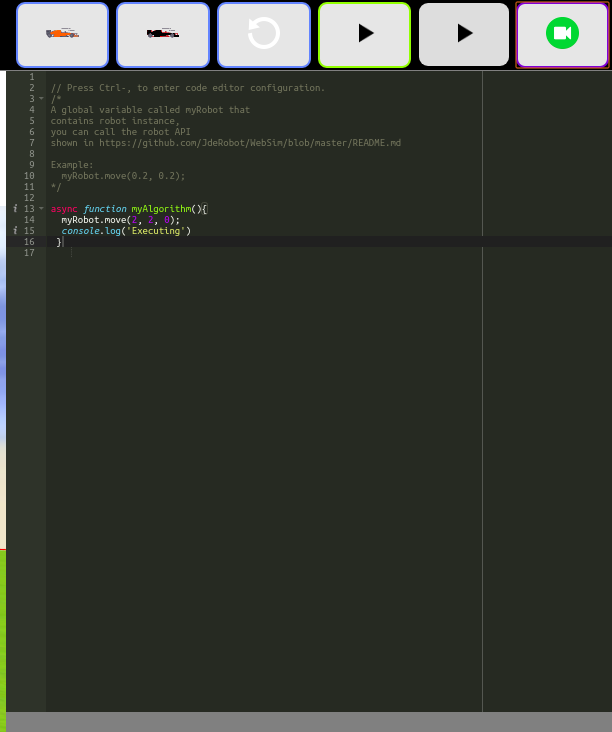
\includegraphics[scale=0.30]{img/competitiveEditorJavascript.png}
        \caption{Editor de \textit{JavaScript} para ejercicios competitivos}
        \label{fig:javascript_competitivo}
    \end{figure}
    
Cada uno de los botones tiene la funcionalidad de guardar el código escrito en el editor y, si se pulsa el botón del robot que no se está editando, se guarda el código y se carga el del otro robot en caso de que ya haya uno guardado. Si no hay ninguno se carga un editor vacío. 

\begin{lstlisting}[language=javascript]
var editFirst = true;
var editSecond = false;
var codeFirst = null;
var codeSecond = null;
  $('#firstRobot').click(()=>{
    if(editFirst){
      codeFirst = editor.getCode();
    }
    if(editSecond){
      codeSecond = editor.getCode();
      editSecond=false;
      if(codeFirst==null){
        editor.insertCode("",editor);
      }else{
        editor.insertCode(codeFirst,editor);
      }
    }
    editFirst= true;
  });
\end{lstlisting}

Cuando se pulsa el botón de ejecutar código, se ejecuta el método \textit{runBrain} del módulo \textit{brains} obteniendo previamente el código del robot que se esté editando.
\begin{lstlisting}[language=javascript]
  $("#runbtn").click(()=>{
     if (editFirst) {
       codeFirst = editor.getCode();
     } else {
       codeSecond = editor.getCode();
     }
    if (brains.threadExists(editorRobot1)){
      if (brains.isThreadRunning(editorRobot1)){
        brains.stopBrain(editorRobot1);
        brains.stopBrain(editorRobot2);
      }else{
        brains.resumeBrain(editorRobot1,codeFirst);
        brains.resumeBrain(editorRobot2,codeSecond);
      }
    }else{
      brains.runBrain(editorRobot1,codeFirst);
      brains.runBrain(editorRobot2,codeSecond);
    }
  });
\end{lstlisting}


La aplicación \textit{web} \textit{competitive-Scratch} se ha realizado de  manera similar, con la diferencia de que en este caso es necesario guardar el código de los bloques en \textit{XML} y su traducción en \textit{JavaScript}. Para realizarlo de forma limpia se ha creado un objeto que contiene un \textit{boolean} y dos cadenas de texto (\textit{listing} \ref{lst:savecode}). En el primero indica el código de qué \textit{robot} se está editando, en una cadena de texto se guarda el código \textit{XML} y en la otra su traducción en \textit{JavaScript}. Se puede ver la interfaz de este editor en la figura \ref{fig:scratch_competitivo}.
    \begin{figure}[H]
        \centering            
        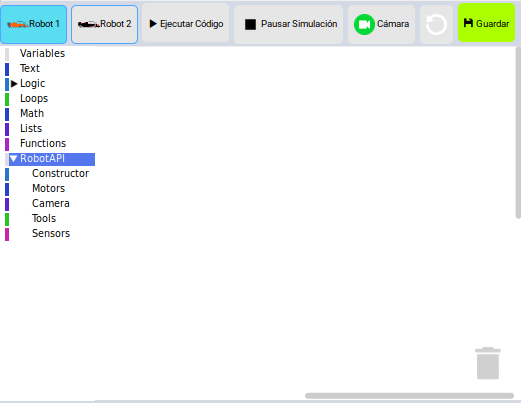
\includegraphics[scale=0.8]{img/competitivoEditorScratch.png}
        \caption{Editor de \textit{Scratch} para ejercicios competitivos}
        \label{fig:scratch_competitivo}
    \end{figure}

\begin{lstlisting}[language=javascript,label=lst:savecode, caption=código \textit{JavaScript} para guardar código de un robot]
var codeFirst = {
  js:"",
  xml:null,
  edit:true
};
var codeSecond = {
  js:"",
  xml: null,
  edit: false
};
  $('#firstRobot').click(()=>{
    if(codeFirst.edit){
      codeFirst.xml = editor.storeCode(editor.ui);
      editor.ui = editor.injectCode(editor.ui, codeFirst.xml);
    }
    if(codeSecond.edit){
      codeSecond.xml = editor.storeCode(editor.ui);
      codeSecond.edit = false;
      if(codeFirst.xml == null){
        editor.ui = editor.injectCode(editor.ui, '<xml></xml>');
      } else{
        editor.ui = editor.injectCode(editor.ui, codeFirst.xml);
      }
    }
    codeFirst.edit = true;
\end{lstlisting}

\begin{lstlisting}[language=javascript,caption=código \textit{JavaScript} para ejecutar código de los robots y guardar el que se está editando]
$("#runbtn").click(()=>{
    if (codeFirst.edit) {
        codeFirst.xml = editor.storeCode(editor.ui);
        editor.ui = editor.injectCode(editor.ui,codeSecond.xml);
        codeSecond.js = editor.getCode();
        editor.ui = editor.injectCode(editor.ui,codeFirst.xml);
        codeFirst.js = editor.getCode();
    } else {
        codeSecond.xml = editor.storeCode(editor.ui);
        editor.ui = editor.injectCode(editor.ui,codeFirst.xml);
        codeFirst.js = editor.getCode();
        editor.ui = editor.injectCode(editor.ui,codeSecond.xml);
        codeSecond.js = editor.getCode();
    }
    if (brains.threadExists(editorRobot1)){
      if (brains.isThreadRunning(editorRobot1)){
        brains.stopBrain(editorRobot1);
        brains.stopBrain(editorRobot2);
      }else{
        brains.resumeBrain(editorRobot1,codeFirst.js);
        brains.resumeBrain(editorRobot2,codeSecond.js);
      }
    }else{
      brains.runBrain(editorRobot1,codeFirst.js);
      brains.runBrain(editorRobot2,codeSecond.js);
    }
  });
\end{lstlisting}

Para puntuar el comportamiento de los robots de manera justa se han incluido en estos ejercicios \textit{evaluadores automáticos}. Van a tener diferentes comportamientos en cada ejercicio, por lo que se han desarrollado de tal forma que se pueda cargar cargar un evaluador distinto para cada uno o, incluso, no cargar ninguno. \newline

Para su implementación se ha creado el módulo \textit{evaluators}, que es similar a \textit{brains}. Tiene un método \textit{runEvaluator}, que acepta como parámetro un \textit{array} con los identificadores de los \textit{robots} a los que el código del evaluador debe conectarse para poder medir la calidad y el archivo del evaluador deseado. Este fichero se recoge como variable en el \textit{index.html} (listing \ref{lst:confEvaluator}) del editor correspondiente de forma similar a los archivos de configuración:
\begin{lstlisting}[language=html,label=lst:confEvaluator]
   <script>var config_evaluator = "evaluator_follow_line.js";</script> 
\end{lstlisting}

Para llamar a \textit{runEvaluator} se comprueba que se haya pasado un fichero en el \textit{index.html} en el código que inicializa el editor correspondiente: 

\begin{lstlisting}[language=html,label=lst:checkFile]
   if(typeof config_evaluator!=="undefined"){
    evaluators.runEvaluator([editorRobot1,editorRobot2],config_evaluator);
  }
\end{lstlisting}

En el método \textit{runEvaluator} se realiza un \textit{require} (que es la forma de importar módulos en \textit{JavaScript} de manera dinámica) de ese fichero, se crea la interfaz gráfica en el método \textit{evaluator.createInterface()} y se crea un objeto en el array de \textit{brains} que se ejecuta cada 400 milisegundos por medio del método \textit{evaluators.createTimeoutEvaluator}, que se apoya en la función \textit{setTimeout} de JavaScript. 


\begin{lstlisting}[language=javascript,caption={Funciones que crean el objeto para ejecutar el evaluador periódicamente}]
evaluators.runEvaluator = (arrayRobots,config_file)=>{
   evaluator = require("../assets/evaluators/"+config_file);
   evaluator.createInterface();
   brains.threadsBrains.push({
     "id": "evaluator",
     "running": true,
     "iteration": evaluators.createTimeoutEvaluator(arrayRobots,"evaluator"),
     "codeRunning": ""
   });
}
evaluators.createTimeoutEvaluator = (arrayRobots,id)=>{
  stopTimeoutRequested = false;
  let brainIteration = setTimeout(async function iteration(){
    evaluator.setEvaluator(arrayRobots);
    if (!stopTimeoutRequested) {
        var t = setTimeout(iteration, 400);
        var threadBrain = brains.threadsBrains.find((threadBrain)=> threadBrain.id == id);
        threadBrain.iteration = t;
    }
  }, 400);
  return brainIteration;
}
\end{lstlisting}


\subsection{Atraviesa-bosque competitivo}
\label{subsec:bosquecmp}
Este ejercicio es similar al escenario con un solo robot, pero en este caso se han creado dos pasillos en lugar de uno\footnote{\url{https://www.youtube.com/watch?v=v_aMvNPtncg}}. Se han añadido distintos objetos y elementos de \textit{A-Frame} en la misma ubicación para los dos \textit{robots} para que el recorrido sea justo.

Para su evaluador se crea una barra de progreso para cada robot y un cronómetro. Cuando se empiezan a mover los robots la barra de progreso empieza a completarse y el cronómetro se inicia, para comprobar el porcentaje completado se obtiene la posición del robot y la compara con el punto de llegada.

\begin{figure}[H]
\centering           
\includegraphics[scale=0.3]{img/evaluador_forest.png}
\caption{Escenario y evaluador para el ejercicio atraviesa-bosque}
\label{fig:evaluador_bosque}
\end{figure}


Las funciones necesarias para el evaluador se definen a continuación: 
\begin{itemize}
    \item Una dedicada a crear la interfaz que establece los elementos necesarios para añadir las barras de progreso, iconos, tiempo y sus atributos.
\begin{lstlisting}[language=javascript]
evaluator.createInterface= ()=>{
  var node = document.createElement("div");
  node.setAttribute("class","evaluator");
  var img1 = document.createElement("img");
  img1.setAttribute("class","carMarker");
  img1.setAttribute("src","../assets/resources/car1.svg")
  node.appendChild(img1);
  var node2 = document.createElement("div");
  node2.setAttribute("id","car1Progress");
  var node3 = document.createElement("div");
  node3.setAttribute("id","a-car1bar");
  node3.innerHTML = "0%";
  node2.appendChild(node3);
  node.appendChild(node2);
  var img2 = document.createElement("img");
  img2.setAttribute("class","carMarker");
  img2.setAttribute("src","../assets/resources/car2.svg")
  node.appendChild(img2);
  var node4 = document.createElement("div");
  node4.setAttribute("id","car2Progress");
  var node5 = document.createElement("div");
  node5.setAttribute("id","a-car2bar");
  node5.innerHTML = "0%";
  node4.appendChild(node5);
  node.appendChild(node4);
  var time = document.createElement("div");
  time.setAttribute("id","time");
  time.innerHTML="Tiempo: 00:00";
  time.style.marginTop="-87px";
  time.style.color="white";
  node.appendChild(time);
  var myiframe= document.getElementById("myIFrame");
  myiframe.insertBefore(node,myiframe.childNodes[0]);
}
\end{lstlisting}
    \item La función que se ejecuta periódicamente comprueba la velocidad de los robots y, si es mayor que 0, se inician los evaluadores, llama a una función que realiza la lógica para actualizar las barras de progreso y añadir un cronómetro al \textit{DOM}. La variable \textit{timeInit} se actualiza constantemente hasta que el usuario ejecuta su código y el \textit{robot} comienza a moverse, que se calcula el tiempo transcurrido y lo muestra en pantalla.
\begin{lstlisting}[language=javascript]
evaluator.setEvaluator = (arrayRobots) =>{
  let robot=Websim.robots.getHalAPI(arrayRobots[0]);
  if(!clock){
    timeInit = new Date();
  }
  if(robot.velocity.x>0){
    clock=true;
    var time= document.getElementById("time");
    progressBar(arrayRobots);
    var realTime = new Date(new Date() - timeInit);
    var formatTime = timeFormatter(realTime);
    time.innerHTML = "Tiempo: " + formatTime;
  }
}
\end{lstlisting}
    \item Función que calcula el porcentaje recorrido por cada uno de los \textit{robots}, modifica las barras de progreso y lo añade al \textit{DOM} para que aparezca en texto.
    
  \begin{lstlisting}[language=javascript]
function progressBar(arrayRobots){
  arrayRobots.forEach(function(robotID){
    let robot = Websim.robots.getHalAPI(robotID);
    var left=38.24 + robot.getPosition().x;
    var completed=(left*100)/78.48;
    var element = document.getElementById(robot.myRobotID+"bar");
    if((100-completed)>100){
      element.style.width = 100 + '%';
      element.innerHTML = 100 + '%';
    }else{
      element.style.width = Math.round(100-completed) + '%';
      element.innerHTML = Math.round(100-completed) + '%';
    }
  });
}
\end{lstlisting}
        \item Función que da formato al cronómetro.
\begin{lstlisting}[language=javascript]
function timeFormatter(time){
  var formatTime;
  if (time.getMinutes()<10){
    formatTime="0"+time.getMinutes();
  }else{
    formatTime=time.getMinutes();
  }
  formatTime+=":";
  if (time.getSeconds()<10){
    formatTime+="0"+time.getSeconds();
  }else{
    formatTime+=time.getSeconds();
  }
  return formatTime;
}
\end{lstlisting}
\end{itemize}

\subsection{Sigue-líneas competitivo}
\label{subsec:race}

En este ejercicio hay dos robots en el que tienen que seguir una linea de color blanco sobre fondo negro atravesando un puente en medio del circuito para que, de esta manera, ambos recorran la misma distancia\footnote{\url{https://www.youtube.com/watch?v=OaA7_wsXhk8}}.

La principal novedad del escenario es el puente creado, que permite ser cruzado mientras siguen la línea. La solución definitiva ha sido creando primitivas de \textit{A-Frame} (\textit{a-plane}) y añadiendo una textura diseñada con \textit{Photoshop} con el mismo aspecto que el resto del circuito.

El evaluador de este ejercicio es similar al de atraviesa-bosque, con la diferencia de que es necesario guardar en todo momento la posición y distancia recorrida por cada robot para calcular el porcentaje del circuito completado. 
\begin{lstlisting}[language=javascript,caption=Objeto creado para guardar posición y distancia recorrida de un robot]
var car={
    pos:{
        x:robot.getPosition().x,
        z:robot.getPosition().z
    },
    dist: 0
}
\end{lstlisting}

 \begin{lstlisting}[language=javascript,caption=Función que realiza la funcionalidad para rellenar la barra de progreso]
evaluator.setEvaluator = (arrayRobots) => {
  let robot1=Websim.robots.getHalAPI(arrayRobots[0]);
  let robot2=Websim.robots.getHalAPI(arrayRobots[1]);
  if(!clock){
    timeInit = new Date();
    car1 = {
        pos:{
                x:robot1.getPosition().x,
                z:robot1.getPosition().z
            },
            dist: 0
    };
    car2 = {
        pos:{
            x:robot2.getPosition().x,
            z:robot2.getPosition().z
        },
        dist: 0
    }
  }
  if(robot1.velocity.x>0){
    clock=true;
    var time= document.getElementById("time");
    progressBar(arrayRobots,[car1,car2]);
    var realTime = new Date(new Date() - timeInit);
    var formatTime = timeFormatter(realTime);
    time.innerHTML = "Tiempo: " + formatTime;
  }
}
\end{lstlisting}
            
\begin{figure}[H]
    \centering           
    \includegraphics[scale=0.2]{img/evaluator_follow_line.png}
    \caption{Ejercicio y evaluador sigue-líneas competitivo}
    \label{fig:evaluador_siguelineas}
\end{figure}

\subsection{Gato-ratón}
\label{subsec:gatoraton}
No es estrictamente hablando un ejercicio competitivo directamente, con dos códigos de estudiantes sobre sendos robots en el mismo escenario simultáneamente. En este ejercicio hay dos robots, uno (el \textit{drone} gato) programado por el estudiante que hace el ejercicio y otro (el \textit{drone} ratón) programado por desarrolladores de la plataforma. 
En este ejercicio el usuario tiene que desarrollar su solución para que el \textit{robot} no se aleje del objetivo, el \textit{drone} ratón, que está en constante movimiento\footnote{\url{https://www.youtube.com/watch?v=xA9Emhdk_HQ}}. 

\begin{figure}[ht]
\centering           
\includegraphics[scale=0.3]{img/evaluador_drone.png}
\caption{Evaluador y escenario con dos robots para ejercicio gato-ratón}
\label{fig:evaluador_gato_raton}
\end{figure}


Para este ejercicio se ha creado un \textit{script} llamado \textit{agents-methods.js}, basado en \textit{brains}, para ejecutar el código del \textit{drone} ratón sin necesidad de escribir código. Es muy similar al método \textit{runBrain} con la diferencia de que el código viene de un fichero en lugar del editor. En este módulo se guarda el código en la variable \textit{agents.code} con el siguiente código: 

\begin{lstlisting}[language=javascript]
agents.getCode = (file) => {
  var request = new XMLHttpRequest();
  request.open("GET", file);
  request.onreadystatechange = function () {
    if(request.status === 200 || request.status == 0) {
        agents.code = request.responseText;
    }
  }
  request.send();
}
\end{lstlisting}

Siendo \textit{file} una variable que se inicializa en el \textit{index.html} de manera similar a los ficheros de configuración y evaluadores automáticos. 
Una vez obtenido el código se llama al método \textit{runAgent} que recoge el código e incorpora la lógica programada en el \textit{array} de \textit{robots} del módulo \textit{brains}.

\begin{lstlisting}[language=javascript]
agents.runAgent = (robotID, code) =>{
  code = 'async function myAlgorithm(){\n'+code+'\n}\nmyAlgorithm();';
  brains.threadsBrains.push({
    "id": robotID,
    "running": true,
    "iteration": brains.createTimeoutBrain(code, Websim.robots.getHalAPI(robotID), robotID),
    "codeRunning": code
  });
}
\end{lstlisting}

A la hora de ejecutar el código, se elige si el código que se ejecuta es el que hay en el agente llamando al método \textit{runAgent} del módulo \textit{agents} o el que hay en el editor con el método \textit{runBrain} del módulo \textit{brains}. \\
En el siguiente código se ejecuta en un \textit{robot} el código escrito en el editor y en otro el escrito en el agente:

\begin{lstlisting}[language=javascript]
  $("#runbtn").click(()=>{
     if (editFirst) {
       codeFirst = editor.getCode();
     } else {
       codeSecond = editor.getCode();
     }
    if (brains.threadExists(editorRobot1)){
      if (brains.isThreadRunning(editorRobot1)){
        brains.stopBrain(editorRobot1);
        brains.stopBrain(editorRobot2);
      }else{
        brains.resumeBrain(editorRobot1,codeFirst);
        agents.resumeAgent(editorRobot2,agents.code);
      }
    }else{
      brains.runBrain(editorRobot1,codeFirst);
      agents.runAgent(editorRobot2,agents.code);
    }
  });\end{lstlisting}
  
  
Para el evaluador de este ejercicio se crea un gráfico con ayuda de una librería externa de \textit{JavaScript} (\textit{JavaScript Graphics Library}\cite{bib:jsgrafico}) que muestra la distancia entre \textit{drones} y el tiempo que lleva de ejecución. Se puede ver este evaluador en la figura \ref{fig:evaluador_gato_raton}. 
 En este caso, el método \textit{createInterface} realiza añade todo lo necesario al \textit{DOM} para que el gráfico sea completo y llama a la función \textit{setAxis()} para añadir los ejes y las etiquetas. \\
 
 \begin{lstlisting}[language=javascript,caption=Función que establece los ejes y etiquetas de la gráfica]
 evaluator.createInterface= ()=>{
  var node = document.createElement("div");
  node.setAttribute("id","panel");
  node.style.height="130px";
  node.style.backgroundColor="white";
  var time = document.createElement("div");
  time.setAttribute("id","time");
  time.marginLeft="50px";
  time.innerHTML="Tiempo: 00:00";
  time.style.color="black";
  time.style.textAlign="center";
  node.appendChild(time);
  var myiframe= document.getElementById("myIFrame");
  myiframe.insertBefore(node,myiframe.childNodes[0]);
  myPanel = new jsgl.Panel(document.getElementById("panel"));
  setAxis(myPanel);
  line = myPanel.createPolyline();
  line.getStroke().setColor('blue');
  line.getStroke().setWeight(2);
}
\end{lstlisting}

\begin{lstlisting}[language=javascript,caption=Método \textit{createInterface}]
function setAxis(myPanel){
  var axisX = myPanel.createLine();
  axisX.setStartPointXY(20,10);
  axisX.setEndPointXY(20,100);
  myPanel.addElement(axisX);
  var axisY = myPanel.createLine();
  axisY.setStartPointXY(20,100);
  axisY.setEndPointXY(500,100);
  myPanel.addElement(axisY);
  var myLabel = myPanel.createLabel();
  myLabel.setLocation(new jsgl.Vector2D(75,100));
  myLabel.setText("00:30");
  myPanel.addElement(myLabel);
  var myLabel = myPanel.createLabel();
  myLabel.setLocation(new jsgl.Vector2D(0,20));
  myLabel.setText("10");
  myPanel.addElement(myLabel);
}
\end{lstlisting}

\begin{lstlisting}[language=javascript,caption={Código JavaScript que calcula la distancia entre \textit{drones}, la representa e incorpora un cronómetro al \textit{DOM}}]
evaluator.setEvaluator = (arrayRobots) => {
  var robot1 = Websim.robots.getHalAPI(arrayRobots[0]);
  var robot2 = Websim.robots.getHalAPI(arrayRobots[1]);
  if(!clock){
    timeInit = new Date();
  }
  if(robot1.velocity.x >0 || robot2.velocity.x>0){
    clock = true;
    var time= document.getElementById("time");
    var realTime = new Date(new Date() - timeInit);
    var formatTime = timeFormatter(realTime);
    time.innerHTML = "Tiempo: " + formatTime;
    var pos1 = robot1.getPosition();
    var pos2 = robot2.getPosition();
    var dist = Math.sqrt(Math.pow(pos2.x-pos1.x,2)+
                         Math.pow(pos2.y-pos1.y,2)+
                         Math.pow(pos2.z-pos1.z,2));
    line.addPointXY(x,dist+10);
    x=x+0.5;
    myPanel.addElement(line);
  }
}
\end{lstlisting}


% SOPORTE LEGO EV3 FISICO %
%%%%%%%%%%%%%%%%%%%%%%%%%%%%%%%%%%%%%%%%%%%%%%%%%%%%%%%%%%%%%%%%%%%%%%%%%%%%%%%%
%\chapter{Soporte del Robot LEGO Ev3 Físico}
\chaptermark{Soporte Físico}
Ahora nos centraremos en cuál ha sido el desarrollo seguido para que el bloque \textit{Ev3} reciba código desde un cliente exterior y pueda ejecutarlo en local. Primero, el \textit{driver} en \textit{Python} que permite a las aplicaciones de los usuarios de \textit{Kibotics} recibir las lecturas de los sensores del robot real u ordenar movimiento a sus motores. Y luego cómo integrarlo de modo que el programa se descargue en el robot real desde la página web de \textit{Kibotics}

\section{Interfaz de programación de sensores y actuadores}
\sectionmark{Interfaz de programación}
\label{sec:interfazfisico}
Para crear los \textit{drivers} de \textit{Kibotics} del robot \textit{LEGO EV3} real se ha utilizado la librería \texttt{ev3dev2} donde se encuentran las funciones necesarias para el control del robot en Python 

\subsection{Soporte de actuadores}
Los motores son los actuadores y la forma de uso de \textit{Kibotics} es la de \textit{Tracción diferencial}, en el cual los motores se mueven a la par. Por lo tanto para crear las funciones  del \textit{HAL API} en Python voy a utilizar la clase \textit{MoveTank} dentro de la librería de \texttt{ev3dev2} \footnote{\url{https://github.com/ev3dev/ev3dev-lang-python}} .
 
\begin{lstlisting}[frame=single,breaklines=true, label=Clase MoveTank caption=Clase MoveTank,  captionpos=b]

class MoveTank(MotorSet):
    """
    Controls a pair of motors simultaneously, via individual speed setpoints for each motor.

    Example:

    .. code:: python

        tank_drive = MoveTank(OUTPUT_A, OUTPUT_B)
        # drive in a turn for 10 rotations of the outer motor
        tank_drive.on_for_rotations(50, 75, 10)
    """
    def __init__(self, left_motor_port, right_motor_port, desc=None, motor_class=LargeMotor):
        motor_specs = {
            left_motor_port: motor_class,
            right_motor_port: motor_class,
        }

        MotorSet.__init__(self, motor_specs, desc)
        self.left_motor = self.motors[left_motor_port]
        self.right_motor = self.motors[right_motor_port]
        self.max_speed = self.left_motor.max_speed
        self._cs = None
        self._gyro = None
\end{lstlisting}

En esta clase se encuentran todos los métodos con los que construiré mi \textit{Driver}


\begin{lstlisting}[frame=single,breaklines=true, label=Driver Actuadores, caption=Drivers,  captionpos=b]


import ev3dev2.motor
import time


class Ev3Wrapper:

    def __init__(self,
                 left_motor_port=OUTPUT_D,
                 right_motor_port=OUTPUT_A):


        tank_drive = MoveTank(left_motor_port, right_motor_port)


    def TurnDegrees(self, degrees, speed):
        # get the starting position of each motor
        tank_drive.turn_degrees(self, speed, degrees)

    def avanzar(self, val):
        tank_drive.on(self,val, val)

    def retroceder(self, val):
        tank_drive.on(self,-val,-val)

    def girar_derecha(self, w):

        tank_drive.turn_right(self, 360, 2*3,1416/w)

    def girar_izquierda(self, w):

        tank_drive.turn_left(self, 360, 2*3,1416/w)

    def avanzar_hasta(self, distance):
        dist_mm = distance * 1000

        # the number of degrees each wheel needs to turn
        tank_drive.on_for_distance(self, 20, distance_mm, brake=True, block=True)

    def retroceder_hasta(self, distance):
        self.avanzar_hasta(-distance)

    def girar_derecha_hasta(self, degrees):
        self.TurnDegrees(degrees, 20)

    def girar_izquierda_hasta(self, degrees):
        self.TurnDegrees(-degrees, 20)

    def parar(self):
        tank_drive.odometry_stop()


    def target_reached(self,left_target_degrees,right_target_degrees):
        tolerance = 5
        min_left_target = left_target_degrees - tolerance
        max_left_target = left_target_degrees + tolerance
        min_right_target = right_target_degrees - tolerance
        max_right_target = right_target_degrees + tolerance

        current_left_position = left_motor_port.position()
        current_right_position = right_motor_port.position()

        if current_left_position > min_left_target and \
           current_left_position < max_left_target and \
           current_right_position > min_right_target and \
           current_right_position < max_right_target:
            return True
        else:
            return False
\end{lstlisting}


\subsection{Soporte de sensores}
Dentro de los sensores soportados por el \textit{HAL API} de \textit{Kibotics} hay algunos que no se pueden aplicar al robot \textit{LEGO EV3} ya que no dispone de sensores, como la cámara o el sensor de Infrarrojos. Por lo que los \textit{drivers} que se incluirán en este apartado son:

\begin{table}[H]
\caption{Métodos (HAL API) soportados por Ev3.}
\vspace{0.5cm}
\label{tab:tablaSensores}
\resizebox{\textwidth}{!}{%
\begin{tabular}{|c|c|c|ll}
\cline{1-3}
\textbf{Método} & \textbf{Descripción} & \textbf{Salida} &  &  \\ \cline{1-3}
.getDistance() & \begin{tabular}[c]{@{}c@{}}Devuelve la distancia entre el robot\\  y la intersección del raycaster en el centro\end{tabular} & number(metros) &  &  \\ \cline{1-3}
.IsTouching() & Devuelve si algo presiona el sensor & Boolean &  &  \\ \cline{1-3}
.getObjectColor(color) & \begin{tabular}[c]{@{}c@{}}Devuelve un objeto con la posición del elemento\\ detectado por la cámara del color pasado por parámetro\end{tabular} & \begin{tabular}[c]{@{}c@{}}\{center:{[}x.y{]},\\ area: int\}\end{tabular} &  &  \\ \cline{1-3}



\end{tabular}%
}
\end{table}

Para este \textit{driver} utilizaré las funciones definidas en el API de \texttt{Ev3dev2.sensor}, las cuales incluyen todas los sensores que puede llevar el \textit{LEGO EV3}. Pero solo utilizaremos las clases \texttt{TouchSensor(), ColorSensor() y Ultrasonic()} que son los tres sensores que usamos en este proyecto. 

\begin{lstlisting}[frame=single,breaklines=true, label=Driver Actuadores, caption=Drivers,  captionpos=b]
from ev3dev2.sensor import INPUT_1, INPUT_2, INPUT_3, INPUT_4
import ev3dev2.sensor.lego
import time


class Ev3Wrapper:

    def __init__(self):
        us= UltraSonic()
        to= TouchSensor()
        cs = ColorSensor()


    def getObjectColor(self, color):
        cs.color()

    def getDistance(self):
        us.distance_centimeters_continuous()

    def isTouching(self):
        to.is_pressed()
\end{lstlisting}

\section{Descarga desde la plataforma}

En la figura se muestra el diseño seguido para integrar el Ev3 real a la plataforma Kibotics. El proceso consta de 4 pasos y en las siguientes secciones se profundizará en cada una de las partes y en las interacciones necesarias entre el cliente, el servidor de Kibotics y el servidor \textit{Flask} que lanzaremos en el \textit{Robot Ev3},lo que permitira programarlo desde el navegador web usando  \textit{Kibotics}.

\begin{figure}[h!]
  \centering
    \includegraphics[width=0.8\textwidth]{img/esquema.JPG}
  \caption{Diseño para la integración del Ev3}
  \label{comunicacion}
\end{figure}

\subsection{Preparación ordenador a bordo del robot}
Lo primero para la recepción de mensajes es tener un dispositivo que pueda recibirlos, en este caso tendremos que instalar en el \textit{LEGO EV3} un sistema operativo que permita desplegar un servidor. Comenzaré hablando del apartado técnico del robot, para entender la solución adoptada. El Bloque \textit{Ev3} es la mejora de su predecesor el \textit{LEGO NXT}, añadiéndole mas potencia, memoria y expandibilidad. Cuenta con un procesador ARM9 a 300 MHz con memoria Flash de 16 MB, 64 MB de RAM y memoria ampliable con tarjetas mini SD hasta 32 GB. Ademas de eso dispone de conexiones \textit{Bluetoooth 2.1} y puerto USB. 

\begin{wrapfigure}{l}{0.3\linewidth}
    \centering
    \includegraphics[width=0.6\linewidth]{img/logo_ev3dev_mono.png}
    \caption{Ev3Dev Logo}
    \label{fig:ev3dev}
\end{wrapfigure}

\textit{Ev3Dev}\footnote{\url{https://www.ev3dev.org/}} es un sistema operativo basado en \textit{Debian-Linux} diseñadoespecialmente para el \textit{LEGO MINDSTORM EV3} , haciendo ingeniería inversa del bloque.\newline
Una vez instalada la imagen en el robot, para tener conexión a Internet hay dos opciones. La más simple es conectar un \textit{Wifi Dongle} al puerto USB del Bloque \textit{Ev3}, y se accede a la red \textit{Wifi} como cualquier ordenador. La segunda opción es conectar por cable el robot a tu ordenador, y conectarlo a la red como una extensión de tu red.\newline
Una vez conectado a Internet, ya puedes conectarte al robot vía \textit{SSH}.

\begin{figure}[h!]
  \centering
    \includegraphics[width=0.8\textwidth]{img/ev3dev.png}
  \caption{Interfaz de la terminal de Ev3}
  \label{Diseño hardware del Ev3}
\end{figure}
Además crearon en \textit{Ev3dev} un entorno de software para programar el robot. Esto incluye soporte para muchos lenguajes de programación, entre ellos \textit{Python, Java o C++}. Para este proyecto he elegido utilizar el lenguaje \textit{Python}, ya que es uno de los lenguajes que comprende \textit{Kibotics} y estoy más familiarizado con él. 

\subsection{WebBrowser}

\subsubsection{Editor en el navegador web}

El editor de texto se encontrará entre la parrilla de ejercicios de \textit{Kibotics}. En este caso \textit{Kibotics} solo actua como plataforma que guarda los ejercicios que envió, y me proporciona la interfaz para poner el editor de texto que permita escribir su programa utilizando el lenguaje \textit{Python}. En el editor se importa la librería “\textit{Ev3dev2}”  que proporciona una API para interactuar con los sensores y actuadores del robot. Pero en este caso, \textit{Kibotics} no actúa en el envío, solo sirve la página para que podamos introducir el código.

\subsubsection{Envío del código al servidor Flask en el robot}

Utilizamos el editor \textit{ACE} para que el usuario escriba su código en la página Web, y cuando le de al botón \texttt{Enviar}, comienza el proceso de envío desarrollado en el script siguiente:
\\
\begin{lstlisting}[frame=single,breaklines=true, label=Función de envío del código al servidor, caption=Función de envío del código al servidor captionpos=b] <center><h3>En esta seccion podras enviar tu codigo  al LEGO Ev3.</h3></center>

<div class="text-center">
 <img class="text-center" src="{{ exercise.language }}/{{ exercise.exercise_id }}/img/ev3.png" width="300px" height="250px">
</div>

<div class="text-center">
  <img class="text-center" src="img/lego-mindstorms-education-ev3.jpg"
      width="300px" height="250px"
</div>

      <button type="button" id="send_mbot" class="btn btn-info" onclick="send_code_to_ev3()"><span
              class="glyphicon glyphicon-send"></span> Enviar
      </button>
</div>
\end{lstlisting}
Tras pulsar el botón \texttt{Enviar}, este código que hemos escrito en el editor se envía como un \textit{query parameter} de una petición POST. Desde el navegador se manda al servidor \textit{Flask} levantado en el robot. 
\\
\begin{lstlisting}[frame=single,breaklines=true, label=Función de envío del código al servidor, caption=Función de envío del código al servidor,  captionpos=b]
let responseOk;

  function send_code_to_ev3() {
      var editor = ace.edit("ace");
      let code = editor.getValue();
      console.log(code);
      const message = {
          method: "POST"
      };
      url = 'http://10.42.0.1:8001/run?python_code=' + JSON.stringify(code);
      fetch(url, message)
          .then(function(response) {
              if(response.ok){
                  responseOk = true
              }else{
                  responseOk = false
              }
              return response.text();
          })
          .then(function(data) {
               if(responseOk){
                  console.log("Ok")
              }else{
                  console.log("Send Fail")
              }

          })
          .catch(function(err) {
              console.error(err);
          });
  }
}
\end{lstlisting}
El servidor \texttt{Flask} hará la recepción del código que escribimos en el editor, y realizará determinadas acciones para que se pueda ejecutar en el \textit{LEGO EV3}


\subsection{Back-End}
El servidor que se ha creado, hace uso de \texttt{Flask} que es un entorno creado por \textit{Django} escrito en \textit{Python}, por lo que voy a programarlo en \textit{Python}. Esta creado para que reciba peticiones del navegador con el código que el usuario escribió en el editor



\begin{lstlisting}[frame=single,breaklines=true, label=Extracción del código en el servidor Flask, caption=Extracción del código en el servidor Flask,  captionpos=b]
import subprocess
import os
import signal
import time

from flask import Flask, make_response, request
app = Flask(__name__)   

exercice = None
@app.route('/run',methods=["POST"])
def run_program():
    global exercice
	my_json = request.data.decode('utf8').replace("'", '"')
    data = json.loads(my_json)
    code = json.dumps(data["code"])
    
    
#----------------------------------------------------------


if __name__ == "__main__":
    app.run(host='0.0.0.0', port=8001, debug=True)
\end{lstlisting}

\subsubsection{Creación del proceso que ejecuta la aplicación robótica}

Una vez ha recibido el código, el servidor ya sabe que el lenguaje en que viene es \textit{Python}, pero viene con algunos simbolos añadidos de HTML, por lo que se realizan dos \textit{replace} para dejarlo como estaba en origen.\newline
Una vez hecho este proceso, se procede a escribir un ejecutable con el código, para ello hay creado un archivo llamado \textit{ejercicio.py}.
Una vez creado el archivo se comprueba que no hay otro proceso ejecutándose, si es así se envía una señal \textit{kill} a dicho proceso.
Tras ejecutar el programa en un nuevo proceso, el robot realizará las instrucciones que el usuario programó en el editor del navegador web.
\\
\begin{lstlisting}[frame=single,breaklines=true, label=Creación del proceso con el programa para el robot, caption=Creación del proceso con el programa para el robot,  captionpos=b]
if exercice:
        try:
            os.killpg(os.getpgid(exercice.pid), signal.SIGKILL)
        except ProcessLookupError:
            pass

    time.sleep(2)
  
    code  = code[1:-1].split("\\n")
    print(code)
    fdOut = open("./ejercicio.py","w")
    for line in code:
            fdOut.write(line + "\n")
    
    exercice = subprocess.Popen(["python","ejercicio.py"],stdout=subprocess.PIPE,preexec_fn=os.setsid)
    
\end{lstlisting}

\subsubsection{Respuesta del Servidor}

Por último, se contesta al cliente con el código \textit{200 OK} 

\begin{lstlisting}[frame=single,breaklines=true, label=Respuesta del Servidor, caption=Creación del proceso con el programa para el robot,  captionpos=b]

headers = {'Content-Type': 'text/plain','Access-Control-Allow-Origin': '*'}
    return make_response('Ok', 200, headers)

\end{lstlisting}



\section{Validación experimental con Ejercicios}
\sectionmark{Validación Experimental}
En esta sección procedo a enviar dos ejercicios programados con las funciones de \textit{Kibotics} en el editor Web  para comprobar que lo que he contado anteriormente funciona. 
\subsection{Ejercicio Bump and go}
Para comprobar que todo lo anterior funciona hice tres ejercicios enviados desde un navegador web y ejecutados en el robot real. El primero, el \textit{BumpandGo} \footnote{\url{https://www.youtube.com/watch?v=5dD7O7Qku6I&ab_channel=DanielPulidoMillanes}} probando los el sensor de contacto.
\\
\begin{figure}[h!]
  \centering
    \includegraphics[width=0.8\textwidth]{img/editor_ev3.png}
  \caption{Editor Web para \textit{LEGO Ev3}}
  \label{Editor Web}
\end{figure}
\clearpage

En este apartado será donde insertemos el código que mandaremos al robot, para el caso del \textit{Bump and Go}:


\begin{lstlisting}[frame=single,breaklines=true, label=Bump and Go, caption=Bump and Go,  captionpos=b]

#!/usr/bin/env python3

import Ev3Wrapper
import time
Ev3 = Ev3Wrapper.Ev3Wrapper()

print("Bump and go!")

while True:
    if Ev3.IsTouching():
    	Eve.retroceder_hasta(10)
        Ev3.girar_derecha_hasta(120)
    else:
        Ev3.avanzar(30)
    # don't let this loop use 100% CPU
    sleep(0.01)

\end{lstlisting}



\subsection{Ejercicio Siguelineas}

El siguiente ejercicio que envié fue el \textit{Siguelineas}\footnote{\url{https://www.youtube.com/watch?v=iMn7UsaB2vo&ab_channel=DanielPulidoMillanes}} para también probar la función \textit{reflectedlightintensity} del sensor de color:
 
 \begin{lstlisting}[frame=single,breaklines=true, label=Siguelineas, caption=SigueLineas,  captionpos=b]

#!/usr/bin/env python3


#!/usr/bin/env python3

import Ev3Wrapper
import time
Ev3 = Ev3Wrapper.Ev3Wrapper()


print("Siguelineas!")

while True:
    while Ev3.getcolor(black)==1:
        Ev3.TurnDegrees(20,15)
    Ev3.TurnDegrees(-20,15)
    # don't let this loop use 100% CPU
    sleep(0.02)

\end{lstlisting}




% CONCLUSIONES %
%%%%%%%%%%%%%%%%%%%%%%%%%%%%%%%%%%%%%%%%%%%%%%%%%%%%%%%%%%%%%%%%%%%%%%%%%%%%%%%%
%\chapter{Conclusiones}
\label{chap:conclusiones}

En este capítulo se recogen las conclusiones a las que se han llegado una vez realizado el Trabajo de Fin de Grado, y voy a valorar los logros alcanzados, comparándolos con los objetivos planteados. Así como una recapitulación sobre los conocimientos adquiridos y se presentarán una serie de mejoras para realizar en un futuro.

\section{Conclusiones}
\label{sec:conclusiones}
El objetivo principal era  integrar el robot \textit{LEGO EV3} en la plataforma de \textit{Kibotics} el cual ha sido alcanzo con exito este objetivo lo dividimos en varios subobjetivos que vamos a ir analizando.

El primer subobjetivo consistía en dar soporte a la parte simulada del robot  \textit{LEGO EV3} en \textit{WebSim}. En el Capitulo 4 se explica cómo se ha llevado a cabo, aportando los modelos en 3D, los \textit{drivers} y bloques para las nuevas funcionalidades que añade el \textit{LEGO EV3}. Entre ellos está el nuevo sensor de contacto con su función \textit{IsTouching} y actualización de la funciones en los \textit{drivers} de los sensores de \textit{Ultrasonidos} y \textit{Sensor de IR}.\\

El segundo subobjetivo era dar soporte al robot real para aceptar código desde el navegador web y el \textit{LEGO EV3} fuera capaz de recibir ese código, interpretarlo y ejecutarlo en local. Para ello se crearon unos \textit{drivers} en Python que daban la funcionalidad al robot real. Para que el robot real pudiera ejecutar programas que le enviaban, necesitó que se le instalara una imagen de ditribución \textit{Linux}, se instaló los \textit{drivers} al \textit{LEGO} y se lanzó un servidor \textit{Flask} que se encargaba de recibir los paquetes \textit{HTTP} que enviaba el navegador Web con el código en \textit{Python}. Una vez recibido se encargaba de guardarlo como ejecutable y lanzarlo en local. Todo esto viene explicado con más detalle en el Capitulo 5\\

El tercer subobjetivo era incluir ejercicios que actuaran como validación experimental de los avances que he ido explicando anteriormente, y además para tener una batería de ejercicios que tener como temario. Se han implementado: \textit{Bump and Go, AtraviesaBosque, SigueLineasIR } para el robot simulado, además del \textit{Bump and Go y SigueLíneas} para el robot real en \textit{Python}

\section{Mejoras futuras}
\label{sec:mejoras_futuras}

La implementación del \textit{LEGO EV3} en \textit{Kibotics} ha supuesto un avance para la plataforma, pero además ha dejado las puertas a futuros proyectos que pueden enriquecer más la plataforma, como por ejemplo:

\begin{itemize}
    \item Añadir el \textit{LEGO EV3} real al catálogo de robots que ofrece \textit{Kibotics} en producción, y que se pueda programar y lanzar desde la propia página web de \textit{Kibotics} en vez de, desde una página externa  
    \item Añadir más ejercicios a la plataforma con los sensores que ofrece \textit{LEGO}, aparte de los que vienen con el paquete \textit{MINDSTORM} como pueden ser el micrófono, el sensor de temperatura, o el sensor de luz ambiental. 
    \item Añadir más montajes con el \textit{LEGO Ev3} de modo que el propio robot simulado tenga un centro de gravedad y pueda caer para que el \textit{girosensor} tenga más utilidad. O que haya un nivel de luz, o temperatura en el escenario, lo que daría mas posibilidades a la hora de crear ejercicios. Añadir mas diseños de modelados 3D de robots de \textit{LEGO EV3} y con ellos crear más tipos diferentes de ejercicios.
 
 \end{itemize} 


\cleardoublepage

%\begin{thebibliography}{99}

    \bibitem{bib:navegadores}
    \textit{Navegadores web más empleados:}

    Mozilla: \url{https://www.mozilla.org/}
    
    Opera: \url{https://www.opera.com/}

    Google Chrome: \url{https://www.google.com/intl/es/chrome/}
    
   \bibitem{bib:ros}
    Willow garage y Stanford Artificial Intelligence Laboratory.
    \textit{Página oficial de ROS.}
    \url{https://www.ros.org/}
    
    \bibitem{bib:orca}
    Sourceforge.
    \textit{Página oficial de ORCA:}
    \url{http://orca-robotics.sourceforge.net/}
    
    \bibitem{bib:orocos}
    Orocos.
    \textit{Página oficial de OROCOS:}
    \url{https://orocos.org/}
    
    \bibitem{bib:gazebo}
    Gazebo.
    \textit{Página oficial de Gazebo:}
    \url{https:http://gazebosim.org/}
    
    \bibitem{bib:secundaria}
    Comunidad de Madrid. %Quien lo escribe
    \textit{Asignatura de robótica en Secundaria.} %Nombre
    SIMO EDUCACIÓN, Octubre 2015. % Periodico y fecha de publicacion
    \url{https://n9.cl/7lqc}. % URL

    \bibitem{bib:scratch}
    MIT Media Lab.
    \textit{Página oficial de Scratch:}
    \url{https://scratch.mit.edu/}
    
    \bibitem{bib:lego}
    LEGO.
    \textit{Página oficial de LEGO programming:}
    \url{https://www.lego.com/es-es/categories/coding-for-kids}
   
    \bibitem{bib:gltf}
    \textit{Documentación sobre glTF:}
    \url{https://github.com/KhronosGroup/glTF}
    
    \bibitem{bib:kibotics}
    Kibotics.
    \textit{Plataforma de Kibotics}
    \url{https:https://kibotics.org/}
    
    \bibitem{bib:mindstorm}
    \textit{Especificaciones Lego Ev3}
    \url{https://www.lego.com/es-es/product/lego-mindstorms-ev3-31313}
    
    \bibitem{bib:flask}
    \textit{Documentación de Flask}
    \url{https://flask.palletsprojects.com/en/1.1.x/}
    
	\bibitem{bib:Django}
    \textit{Documentación de Django}
    \url{https://www.djangoproject.com/es}

    \bibitem{bib:aframe}
    Diego Marcos, Don McCurdy, Kevin Ngo. Supermedium, Google y WebVR.
    \textit{Documentación A-Frame.}
    \url{https://aframe.io/}. 

    \bibitem{bib:blockly}
    Google.
    \textit{Documentación Blockly.}
    \url{https://developers.google.com/blockly}
    
    \bibitem{bib:wwwschools}
    Refsnes Data.
    \textit{Documentación para el desarrollo web.}
    \url{https://www.w3schools.com/}
    

\end{thebibliography}
\end{document}
